%--------------------PAQUETES-------------------------------------
\documentclass[openany,12pt,letterpaper]{book}
\usepackage[a4paper]{geometry}
\geometry{left=3cm}
\geometry{right=3cm}
\usepackage[spanish,es-tabla]{babel}
%\usepackage{geometry} % Used to adjust the document margins
\usepackage{graphicx}
\usepackage{listings}
\usepackage[inline]{enumitem} 
\usepackage[normalem]{ulem}
\usepackage{easylist}
\usepackage{bbding}
\useunder{\uline}{\ul}{}
\usepackage[table,xcdraw]{xcolor}
\usepackage{bbding}
\usepackage{standalone}
\setlength{\parskip}{0.5em}
\usepackage[breakable]{tcolorbox}
\usepackage{upquote} % Upright quotes for verbatim code
\usepackage{fancyvrb} % verbatim replacement that allows latex
\usepackage{upquote} % Upright quotes for verbatim code
\usepackage{grffile} % extends the file name processing of package graphics 
\usepackage{longtable} % longtable support required by pandoc >1.10
\usepackage{booktabs}  % table support for pandoc > 1.12.2
\usepackage{float}
\floatplacement{figure}{H} % forces figures to be placed at the correct location
\usepackage{xcolor} % Allow colors to be defined
\usepackage{geometry} % Used to adjust the document margins
\usepackage{amsmath} % Equations
\usepackage{amssymb} % Equations
\usepackage{textcomp} % defines textquotesingle
\usepackage{grffile} % to support a larger range
\usepackage{booktabs}  % table support for pandoc > 1.12.2
\usepackage[normalem]{ulem}
\usepackage[pdftex]{hyperref}
\usepackage{mathrsfs}
\usepackage{multicol}
\usepackage{threeparttable}
\usepackage[bottom]{footmisc}


%------------------VISITADOR-------------------------------------------------
\hypersetup{
	colorlinks=true,
	linkcolor=black,
	filecolor=magenta,      
	urlcolor=cyan,
	bookmarks=true,
	citecolor=blue
}

%--------------------AUTORES--------------------------------------
\title{METODOLOGÍA PARA LA APLICACIÓN DE LA CIENCIA DE DATOS EN EL DIAGNÓSTICO DEL CÁNCER DE MAMA }
\author{Jorge Armando Millán Gomez}

%--------------------TABLAS---------------------------------------
\begin{document}
	\maketitle
	%titlepage
	\thispagestyle{empty}
	\begin{center}
		\begin{minipage}{0.75\linewidth}
			\centering
			%University logo
			
\includegraphics[width=0.3\linewidth]{IMAGENES/LogoUdistrital}
			\par\vspace{2cm}
			%Thesis title
			{\uppercase{\Large METODOLOGÍA PARA LA APLICACIÓN DE LA CIENCIA DE DATOS EN EL DIAGNÓSTICO DEL CÁNCER DE MAMA \par}}
			\vspace{3cm}
			%Author's name
			{\Large Jorge Armando Millán Gómez \par}
			\vspace{3cm}
			%Degree
			{\Large Maestría en Ciencias de la Información y las Comunicaciones énfasis en Ingeniería de Software\par}
			\vspace{3cm}
			%Date
			{\Large \today}
		\end{minipage}
	\end{center}
	\clearpage
	\tableofcontents
	\listoffigures
	\listoftables
	%--------------------[I]PROYECTO----------------------------------
	\part{TESIS DE INVESTIGACIÓN}
	\section*{Introducción}
El Cáncer de mama ocupa el primer lugar con mayor número de muertes en Colombia ocupando el primer puesto en la tasa de letalidad sobre los demás tipos de cáncer afectando a mujeres de todas las edades. En el año 2020 los casos detectados de cáncer de mama en Colombia fueron 15.509 de los cuales 4.411 terminaron en muerte\cite{InternationalAgencyforResearchonCancer2020}. Este tipo de cáncer se origina cuando las células mamarias comienzan a crecer sin control convirtiéndose en células malignas que normalmente forman un tumor que a menudo se puede observar en una radiografía o se puede palpar como una masa o bulto\cite{Sauer2019}. El pronóstico anticipado de esta enfermedad se ha convertido en una necesidad de investigación debido a que puede facilitar el tratamiento preventivo para evitar su letalidad en un estado avanzado. Muchos investigadores han puesto sus esfuerzos en los diagnósticos y pronósticos del cáncer de mama, cada técnica tiene una tasa de precisión diferente que varía según las diferentes situaciones, herramientas y conjuntos de datos que se utilizan. En la actualidad la ciencia de datos es utilizada por diferentes investigadores para modelar la progresión y el tratamiento de afecciones cancerosas debido a su capacidad para detectar características significativas en conjuntos de datos complejos. La medicina basada en datos tiene la capacidad no solo de mejorar la velocidad y precisión del diagnóstico de enfermedades genéticas, sino también de desbloquear la posibilidad de tratamientos médicos personalizados\cite{Baker2018}. Una parte fundamental de la ciencia de datos es el uso de algoritmos de ML\footnote{Machine Learning} y DL\footnote{Deep Learning} los cuales se componen de tres estrategias principales que consisten en preprocesamiento, extracción de características y clasificación. La extracción de características es fundamental en el diagnóstico del cáncer de mama ya que ayuda a identificar datos relevantes en una categoría maligna o benigna\cite{Fatima2020}. Adicionalmente, en los últimos años, el aumento de la potencia de las computadoras, junto con los avances matemáticos, ha permitido el uso de las redes neuronales complejas de múltiples capas (profundas) las cuales han mejorado el rendimiento de la interpretación automática de imágenes oncológicas altamente estandarizadas\cite{Mann2020}.

En otra instancia la literatura muestra que la mayoría de los casos de estudio de investigación científica y de desarrollo de aplicaciones se han dado sobre la aplicación de estas diferentes técnicas a imágenes médicas. Asimismo, otra forma de obtener información relevante es a través de técnicas de detección por Biopsia como es el caso de la aspiración por aguja Fina (FNA\footnote{Fine Needle Aspiration}) y aspiración por aguja gruesa (CNB\footnote{Core Needle Biopsy}) y las técnicas basadas en el análisis de receptores de estrógeno en datos metabolómicos. 
\\\\
Esta investigación se va centrar esencialmente en diseñar una metodología aplicada a técnicas en ciencias de datos partiendo del análisis de un data-set conformado por dicha información para poder comprobar la efectividad de estos métodos médicos en la detección y el diagnóstico del cáncer de mama, lo que nos permitirá evaluar la validez de tener imágenes diagnosticas u otros tipos de datos oncológicos. Esto va a repercutir, en la facilidad de la obtención de los datos y el procesamiento de la información para el diagnóstico y pronostico del padecimiento de esta enfermedad.

	\newpage
\chapter{Estado del arte y Marco Teórico}

\section{Marco teórico}

El eje central esta investigación está basada principalmente en metodologías en ciencia de datos y las técnicas que la componen, tales como:  Machine Learning (ML), Deep Learning (DL), Inteligencia Artificial (IA) y los diferentes métodos estadísticos para comprobación de la hipótesis con base a la diagnosis del cáncer de mama. Dado lo anterior, a continuación se describen los conceptos teóricos relacionados con el tema de estudio:   

\subsection{Detección y diagnóstico del cáncer de mama}
El cáncer de mama, con su causa incierta, ha capturado la atención de los cirujanos en todas las épocas. A pesar de siglos de laberintos teóricos y preguntas científicas, el cáncer de mama aún es una de las enfermedades humanas más temibles \cite{Bland2009}. Según \cite{Fatima2020}, el cáncer de mama se origina a través de tumores malignos, cuando el crecimiento de la célula se descontrola provocando que muchos tejidos grasos y fibrosos de la mama inicien un crecimiento anormal, lo cual tiene como consecuencia que las células cancerosas se diseminen por los tumores causando las diferentes etapas del cáncer. \cite{Fatima2020} exponen que existen diferentes tipos de cáncer de mama \cite{Sun2017}, que se producen cuando las células afectadas y tejidos diseminados se esparcen por todo el cuerpo. Pongamos por caso, el primer tipo de cáncer denominado \textit{Carcinoma ductal in situ (DCIS)} el cual es un tipo de cáncer no invasivo \cite{Hou2020}, que se produce cuando las células anormales se propagan fuera de la mama. El segundo tipo de cáncer es el \textit{Carcinoma ductal invasivo (IDC)}, también conocido como carcinoma ductal infiltrante \cite{Chaudhury2011}. Este tipo de cáncer ocurre cuando las células anormales de la mama se diseminan por todos los tejidos mamarios. Generalmente este tipo de cáncer se encuentra en los hombres \cite{Page1982}. El tercer tipo de cáncer es el cáncer de \textit{Tumores mixtos (MDLC)} también conocido como cáncer de mama invasivo \cite{Tuck1997} causado por las células anormales de los conductos y las células lobulillares \cite{Lee2017}. El cuarto tipo de cáncer es el cáncer de mama \textit{Lobulillar (ILC)} \cite{Masciari2007} que ocurre dentro del lóbulo mamario y aumenta las posibilidades de otros cánceres invasivos. El quinto tipo cáncer es el cáncer de mama \textit{Mucinoso (MBC)} o de \textit{mama coloide} \cite{Memis2000} que ocurre debido a las células ductales invasivas cuando los tejidos anormales se extienden alrededor del conducto \cite{Gradilone2011}. El sexto y ultimo tipo de cáncer es el cáncer de mama \textit{inflamatorio (IBC)}, el cual causa hinchazón y enrojecimiento del pecho. Este tipo de cáncer de mama es de rápido crecimiento, y comienza a aparecer cuando los vasos linfáticos se obstruyen en células rotas \cite{Robertson2010}.

Según \cite{Brunicardi2010}, en la mayoría de casos detectados la mujer descubre una tumoración en su mama. Otros signos y síntomas que se presentan menos a menudo comprenden: crecimiento o asimetría de la mama, alteraciones y retracción del pezón o telorrea, ulceración o eritema de la piel de la mama, una masa axilar y molestia musculoesquelética. Cabe señalar, que si se detectan alguno de los síntomas anteriores este tipo de cáncer puede ser diagnosticado por medio de los procedimientos basados en \textit{Exploración Física}, \textit{Técnicas de imagen} y \textit{Biopsias}. 

A nivel de \textit{Exploración física}, el cáncer de mama puede ser detectado por el oncólogo por medio de los métodos de \textit{Inspección} y \textit{Palpación}. Con estos métodos, se registran la simetría, el tamaño y la forma de la mama, así como cualquier evidencia de edema (piel de naranja), retracción del pezón o de la piel y eritema .

En la actualidad, muchas \textit{Técnicas de imagen} se utilizan ampliamente para proporcionar un diagnóstico preciso de las lesiones mamarias\cite{Tamam2021}, entre estas técnicas las mas relevantes son las siguientes: \textit{La Mamografía} que hace uso de una unidad mamográfica que consta de un tubo de rayos X que encapsula un cátodo y un ánodo. La mama se coloca sobre el detector y se comprime mediante un dispositivo de placas paralelas, el cual mantiene la mama inmóvil y evita el desenfoque por movimiento, esto con el propósito de reducir el grosor del tejido que deben atravesar los rayos x \cite{Ebrahimi2019}; \textit{La ductografía} que identifica de lesiones en pacientes con secreción del pezón. Este método es eficaz para localizar e identificar las lesiones intraductales por medio de un examen mamográfico realizado tras el llenado retrógrado de los conductos galactóforos con material de contraste \cite{Hirose2007}; \textit{La Ecografía} que permite obtener imágenes de alta resolución por medio de un pequeño transductor (sonda) de alta frecuencia que envía ondas sonoras inaudibles al interior de la mama y recibe el eco de las ondas procedentes de los órganos internos, los fluidos y los tejidos \cite{Hasan2019}; y \textit{La Resonancia Magnética (MRI)}que es utilizada cuando las lesiones en la mama no se pueden evaluar fácilmente mediante otras técnicas. Para lograrlo, utiliza bobinas receptoras de radiofrecuencia (RF) para detectar una señal emitida por los tejidos tras la excitación de un campo electromagnético que obliga a los protones alinearse a la anatomía de la zona de interés en tamaño y forma \cite{Tse2014}.

Hay que mencionar, además que actualmente existen dos modalidades para obtener un diagnóstico por \textit{Biopsia} para un paciente que presenta una anomalía mamaria. Por un lado tenemos, la biopsia para mamas con \textit{lesiones palbables} tambien denominada \textit{percutánea} o \textit{mínimamente invasiva}. Estas biopsias incluyen la aspiración con aguja fina (FNA) y con con aguja gruesa (CNB). Las biopsias quirúrgicas abiertas se denominan a veces biopsias por escisión o biopsias por incisión. La biopsia por \textit {escisión} indica la extirpación completa de la lesión, mientras que la biopsia por \textit {incisión} indica la extirpación de parte de la lesión \cite{Greenfield2012}. En el caso de las \textit{lesiones no palpables}, las modalidades de imagen como la ecografía (US), la mamografía y la resonancia magnética (MRI) son complementos útiles para identificar y localizar la lesión de interés. La decisión de cuándo realizar una biopsia de mama depende de los antecedentes del paciente, los hallazgos de la exploración física y las imágenes radiológicas. El objetivo principal de la biopsia es obtener un diagnóstico tisular que pueda ayudar a dictar el tratamiento y la planificación preoperatoria, si está indicado. Por lo tanto, es imprescindible elegir una técnica de biopsia que optimice las posibilidades de obtener un diagnóstico preciso y que, al mismo tiempo, minimice los costes, limite las molestias del paciente y reduzca la necesidad de repetir el procedimiento \cite{Samilia2018}.

\newpage
\subsection{Ciencia de Datos}
La ciencia, en el lenguaje del método científico,es:
\begin{itemize}
	\item Formular hipótesis o conjeturas sobre cómo funciona el mundo, basadas en observaciones del mundo que nos rodea.
	\item Validar o invalidar esas hipótesis mediante la realización de experimentos.
\end{itemize}                   
Sin embargo, a diferencia de las ciencias puras, trabajar con datos no requiere necesariamente realizar experimentos. Más bien, muchas veces los datos ya han sido recopilados y organizados previamente. Entonces, el método científico, aplicado a los datos, se puede resumir como: \textit{“Formular hipótesis basadas en el mundo que nos rodea y luego analizar los datos relevantes para validar o invalidar dichas hipótesis”}. 

\subsection{Machine Learning(ML)}
Aprender significa: \textit{“Adquirir conocimientos o habilidades en algo a través de la experiencia”}.  Por lo tanto, se podría enmarcar al ML cómo la manera en la cual una máquina gana o adquiere conocimiento a través de la experiencia. Pero ¿Cómo adquiere experiencia una máquina? Todas las entradas de una máquina son esencialmente cadenas binarias de 0 y 1, que en el dominio de las ciencias de la computación dichos binarios son simple y llanamente Datos. Por consiguiente, el ML es realmente la forma en que una computadora adquiere conocimiento a través de los datos.  

La ciencia de datos es fundamentalmente un proceso, mientras que el Machine Learning es una herramienta que puede ser inmensamente útil para llevar a cabo el proceso dicho proceso\cite{Pillai2020}. Por supuesto, esto no da ninguna idea del como en absoluto; simplemente se resume el proceso como algo que se hace con los datos de entrada para generar este conocimiento como salida. Para hacer una analogía matemática, el ML es una función $f$ tal que:

\begin{equation}
	Conocimiento=f(Datos)
\end{equation}

Entonces, $f$ podría ser tan mecánico como una simple función matemática. Más específicamente, el ML es mecánico en el sentido de que la forma en que estos algoritmos aprenden se basa estrictamente en principios matemáticos. Por ejemplo, la regresión lineal es un algoritmo que aprende ajustando los coeficientes de los datos de entrada para predecir mejor un valor de salida. La forma en que cambian los coeficientes se basa completamente en protocolos matemáticos (en este caso, los gradientes de los datos de entrada)\cite{Pillai2020}. Y en la práctica, esta es la esencia de la mayoría de los algoritmos comunes de ML, los cuales se clasifican en:

\subsubsection{Aprendizaje Supervisado}
Se refiere a un tipo de modelos de Machine Learning que se entrenan con un conjunto de ejemplos en los que los resultados de salida son conocidos. Los modelos aprenden de esos resultados y realizan ajustes en sus parámetros interiores para adaptarse a los datos de entrada. Una vez el modelo es entrenado adecuadamente, y los parámetros internos son coherentes con los datos de entrada y los resultados del conjunto datos de entrenamiento, el modelo podrá realizar predicciones adecuadas ante nuevos datos no procesados previamente\cite{Roman2019}. Este tipo de aprendizaje está conformado de las siguientes técnicas:

\begin{enumerate}[label=\textbf{\arabic*})]
	
	\item \textbf{Regresión}
	
	La regresión se utiliza para asignar categorías a datos sin etiquetar. En este tipo de aprendizaje tenemos un número de variables predictoras (explicativas) y una variable de respuesta continua (resultado), y se tratará de encontrar una relación entre dichas variables que nos proporcione un resultado continuo\cite{Roman2019}. Los modelos de Regresión más conocidos son los siguientes:
	\begin{enumerate}[label=\textbf{(\alph*)}]
		\item \textit{\textbf{Regresión Lineal:}}
		Se utiliza para estimar los valores reales (costo de las viviendas, el número de llamadas, ventas totales, etc.) basados en variables continuas. La idea es tratar de establecer la relación entre las variables independientes y dependientes por medio de ajustar una mejor línea recta con respecto a los puntos\cite{BriegaLopez2015}. 
		
		\item \textit{\textbf{Regresión Logística:}}
		Los modelos lineales, también pueden ser utilizados para clasificaciones; es decir, que primero ajustamos el modelo lineal a la probabilidad de que una cierta clase o categoría ocurra y, a luego, utilizamos una función para crear un umbral en el cual especificamos el resultado de una de estas clases o categorías. La función que utiliza este modelo es denominada regresión logística\cite{BriegaLopez2015}.  
	\end{enumerate}
	
	\newpage
	\item \textbf{Clasificación}
	
	La Clasificación es una sub-categoría de aprendizaje supervisado en la que el objetivo es predecir las clases categóricas con base a un conjunto de datos existentes\cite{BriegaLopez2015}. Los modelos de clasificación más conocidos son los siguientes:
	
	\begin{enumerate}[label=\textbf{(\alph*)}]
		\item \textit{\textbf{Árboles de decisión:}}
		Los árboles de decisión (DT\footnote{Decision Tree}) son diagramas con construcciones lógicas, muy similares a los sistemas de predicción basados en reglas, que sirven para representar y categorizar una serie de condiciones que ocurren de forma sucesiva, para la resolución de un problema\cite{Roman2019}. 
		
		\item \textit{\textbf{Bosque aleatorio:}}
		La idea central detrás del algoritmo de Bosque aleatorio(RF\footnote{Random Forest}) es construir una gran cantidad de árboles de decisión y luego seleccionar y comparar la categoría que cada árbol eligió\cite{Roman2019}. 
		
		\item \textit{\textbf{Vecinos más cercanos:}}
		Los vecinos mas cercanos (KNN\footnote{K-Nearest Neighborhood}) es un método de clasificación no paramétrico, que estima el valor de la probabilidad a posteriori de que un elemento $x$ pertenezca a una clase en particular a partir de la información proporcionada por un conjunto de datos .Cuando se requiere un resultado para una nueva instancia de datos, el algoritmo KNN recorre dicho conjunto para encontrar las $k$ instancias más cercanas a la nueva instancia, o el número $k$ de instancias más similares al nuevo registro, y luego genera la media de los resultados (para un problema de regresión) o la moda para un problema de clasificación\cite{Shaw2019}.
		
		\item \textit{\textbf{Máquinas de vectores de soporte:}}La maquina de vectores de soporte (SVM\footnote{Support Vector Machine}) es clasificador discriminativo definido formalmente por un hiperplano separador que dados los datos de entrenamiento conocidos genera un hiperplano óptimo que categoriza nuevos registros. En un espacio bidimensional, este hiperplano es una línea que divide un plano en dos partes, donde en cada clase se encuentra a cada lado. En otras palabras, las máquinas de vectores de soporte calculan un límite de margen máximo que conduce a una partición homogénea de todos los puntos de datos\cite{Patel2017}. 
	\end{enumerate}
	
\end{enumerate}

\clearpage
\subsubsection{Aprendizaje No supervisado}
En el aprendizaje No supervisado, se trabaja con datos sin etiquetar cuya estructura es desconocida. El objetivo será la extracción de información significativa, sin la referencia de variables de salida conocidas, y mediante la exploración de la estructura de dichos datos sin etiquetar\cite{BriegaLopez2015}.Este tipo de aprendizaje está conformado de las siguientes técnicas:
\begin{enumerate}[label=\textbf{\arabic*})]
	
	\item \textbf{Agrupamiento(Clustering)}
	El agrupamiento es una técnica exploratoria de análisis de datos, que se usa para organizar información en grupos sin tener conocimiento previo de su estructura. Cada grupo es un conjunto de objetos similares que se diferencia de los objetos de otros grupos. El objetivo es obtener un número de grupos de características similares\cite{BriegaLopez2015}. Los modelos de Clustering más conocidos son los siguientes:
	
	\begin{enumerate}[label=\textbf{(\alph*)}]
		\item \textit{\textbf{K-means :}}
		Es un algoritmo diseñado para dividir datos no etiquetados en un cierto número ($k$) de agrupaciones distintas. En otras palabras, k-means encuentra observaciones que comparten características importantes, las une y las clasifica en grupos\cite{Jeffares2019}. 
		
		\item \textit{\textbf{K-modes:}}
		El algoritmo de agrupación de k-modes es una extensión del algoritmo k-means. Este algoritmo fue diseñado para agrupar grandes conjuntos de datos categóricos, y tiene como objetivo obtener las k modas que representan a un conjunto de datos determinado\cite{Ramirez2020}.
	\end{enumerate}
	
	\item \textbf{Reducción dimensional}
	
	Es común trabajar con datos en los que cada observación se presenta con alto número de características, en otras palabras, que tienen alta dimensionalidad. Este hecho es un reto para la capacidad de procesamiento y el rendimiento computacional de los algoritmos de Machine Learning. La reducción dimensional es una de las técnicas usadas para mitigar este efecto. Este modelo funciona encontrando correlaciones entre las características, lo que implica que existe información redundante, ya que alguna característica puede explicarse parcialmente con otras. Estas técnicas eliminan ruido de los datos, y comprimen los datos en un sub-espacio más reducido, al tiempo que retienen la mayoría de la información relevante\cite{BriegaLopez2015}. El modelos de Reducción Dimensional más conocido es el siguientes:
	
	\begin{enumerate}[label=\textbf{(\alph*)}]
		\item \textit{\textbf{Análisis de componentes principales:}}
		El análisis de componentes principales (PCA\footnote{Principal Component Analysis}) se utiliza para facilitar la exploración y visualización de los datos al reducir el número de variables. Esto se hace capturando la varianza máxima en los datos en un nuevo sistema de coordenadas con ejes llamados componentes principales. Cada componente es una combinación lineal de las variables originales y es ortogonal entre sí. La ortogonalidad entre componentes indica que la correlación entre estos componentes es cero\cite{Shaw2019}.
	\end{enumerate}
	
\end{enumerate}

\subsubsection{Aprendizaje por Refuerzo}

El aprendizaje por refuerzo es una de las ramas más importantes del aprendizaje profundo. El objetivo es construir un modelo con un agente que mejora su rendimiento, basándose en la recompensa obtenida del entorno con cada interacción que se realiza. La recompensa es una medida de lo correcta que ha sido una acción para obtener un objetivo determinado. El agente utiliza esta recompensa para ajustar su comportamiento futuro, con el objetivo de obtener la recompensa máxima\cite{BriegaLopez2015}. 

\subsection{Deep Learning(DL)}

El aprendizaje profundo o Deep Learning, es un sub-campo del ML, que usa una estructura jerárquica de Redes Neuronales Artificiales(ANN\footnote{Artificial Neural Network}), que se construyen de una forma similar a la estructura neuronal del cerebro humano. Esta arquitectura permite abordar el análisis de datos de forma no lineal\cite{BriegaLopez2015}.  Las técnicas utilizadas en el aprendizaje profundo son los siguientes:

\subsubsection{Redes Neuronales}
Al igual que el cerebro humano, las Redes Neuronales constan de neuronas. Cada neurona recibe señales como entrada, las multiplica por pesos, las suma y aplica una función no lineal. Estas neuronas se apilan una al lado de la otra y se organizan en capas\cite{Karagiannakos2020}. La primera capa de la red neuronal toma datos en bruto como entrada, los procesa, extrae información y la transfiere a la siguiente capa como salida. Este proceso se repite en las siguientes capas, cada capa procesa la información proporcionada por la capa anterior, y así sucesivamente hasta que los datos llegan a la capa final, que es donde se obtiene la predicción. Esta predicción se compara con el resultado conocido, y así por análisis inverso el modelo es capaz de aprender los factores que conducen a salidas adecuadas\cite{BriegaLopez2015}.  Las Redes Neuronales se componen de los siguientes algoritmos:

\begin{enumerate}[label=\textbf{\arabic*})]
	
	\item \textbf{Backpropagation}
	
	Las Redes Neuronales pueden aprender una función deseada utilizando grandes cantidades de datos y un algoritmo iterativo llamado \textit{Backpropagation}.  En este caso se alimenta la red con datos, se produce una salida, se compara esa salida con la deseada (usando una función de pérdida) y se reajustan los pesos en función de la diferencia\cite{Karagiannakos2020}.
	
	\item \textbf{Redes Neuronales Feedforward }
	
	Las Redes Neuronales Feedforward (FNN\footnote{Feedforward Neural Network}) suelen estar completamente conectadas , lo que significa que cada neurona de una capa está conectada con todas las demás neuronas de las siguientes capas. La estructura descrita se llama perceptrón multicapa y se originó en 1958. El perceptrón de una sola capa solo puede aprender patrones linealmente separables, pero un perceptrón multicapa es capaz de aprender relaciones no lineales entre los datos. Son excepcionalmente buenos en tareas como clasificación y regresión. A diferencia de otros algoritmos de ML, no convergen tan fácilmente. Cuantos más datos tengan, mayor será su precisión\cite{Karagiannakos2020}.
	
	\item \textbf{Redes Neuronales Convolucionales}
	
	Las Redes Neuronales Convolucionales(CNN\footnote{Convolutional Neural Network}) emplean una función llamada convolución. El funcionamiento de este tipo de redes consiste en que en lugar de conectar cada neurona con todas las siguientes, se conectan con solo con una parte de ella denominada campo receptivo. En cierto modo se intenta regularizar a las redes de retro-alimentación para evitar el sobre-ajuste. Esta característica hace que esta red sea muy buena para identificar relaciones espaciales entre los datos. Es por eso que su caso de uso principal es la visión por computadora y aplicaciones como clasificación de imágenes, reconocimiento de vídeo, y análisis de imágenes médicas\cite{Karagiannakos2020}.
	
	\item \textbf{Redes Neuronales Recurrentes}
	
	Las Redes Neuronales Recurrentes(RNN\footnote{Recurrent Neural Network}) se utilizan para datos relacionados con el tiempo. La retro-alimentación se maneja en forma de bucle desde la salida a la entrada para pasar información a la red. Por lo tanto, son capaces de recordar datos pasados y utilizar esa información en su predicción. Para lograr un mejor rendimiento, los investigadores han modificado la neurona original en estructuras más complejas, como unidades GRU\footnote{Gated Recurrent Units} y unidades LSTM\footnote{Long Short-Term Memory}. Las unidades LSTM se han utilizado ampliamente en el procesamiento del lenguaje natural en tareas como traducción de idiomas, generación de voz y síntesis de texto a voz\cite{Karagiannakos2020}.
	
	\item \textbf{Redes Neuronales Recursivas}
	
	Las Redes Neuronales Recursivas (RNR\footnote{Recursive Neural Network}) son otra forma de redes recurrentes con la diferencia de que están estructuradas en forma de árbol. Como resultado, pueden modelar estructuras jerárquicas en el conjunto de datos de entrenamiento. Se utilizan tradicionalmente en aplicaciones como la transcripción de audio a texto y el análisis de sentimientos debido a sus vínculos con árboles binarios, contextos y analizadores basados en lenguaje natural. Sin embargo, su desempeño tiende a ser mucho más lento en comparación que las redes recurrentes\cite{Karagiannakos2020}.
\end{enumerate}

\subsection{Prueba de Hipótesis}
Una prueba de hipótesis es una prueba estadística que se utiliza para determinar si hay suficiente evidencia en una muestra de datos para inferir que una determinada condición es verdadera para toda la población. Lo que hace la prueba de hipótesis es proporcionar un camino a seguir por el cual se puede probar la hipótesis planteada de manera efectiva. Una prueba de hipótesis examina dos hipótesis opuestas sobre una población: la hipótesis nula y la hipótesis alternativa\cite{Aggarwal2018}. 


\subsubsection{Hipótesis nula ($H_{0}$)}

La hipótesis nula establece que un parámetro de población es igual a un valor. La hipótesis nula es a menudo una afirmación inicial que los investigadores especifican utilizando investigaciones o conocimientos previos\cite{Aggarwal2018}.

\subsubsection{Hipótesis alternativa ($H_{1}$)}

La hipótesis alternativa establece que el parámetro de población es diferente al valor del parámetro en la hipótesis nula. La hipótesis alternativa es lo que se podría creer que es cierto o esperar que sea cierto. Según los datos de la muestra, la prueba determina si se rechaza la hipótesis nula. Utiliza un valor p para hacer la determinación. Si el valor p es menor o igual que el nivel de significancia, que es un punto de corte definido, entonces se puede rechazar la hipótesis nula\cite{Aggarwal2018}.

\newpage
\section{Marco de referencia}
El proposito de esta investigación es proponer una metodología en ciencia de datos y no una técnica de ML y DL. De acuerdo con lo anterior, en la literatura científica no existe información de metodologías para la aplicación de la ciencia de datos en el diagnostico del cáncer de mama, sin embargo se encontraron metodologías cuyas etapas pueden ser utilizadas en proyectos enfocados en las ciencias de la salud. Por otra parte, en las investigaciones analizadas se encontró bastante información de técnicas de ML y DL para el diagnostico esta enfermedad. Por esta razón, a continuación se presentan las metodologías en ciencia de datos relevantes para el tema de estudio y las técnicas en ML y DL mas destacadas en la comunidad científica.  

\subsection{Metodologías en ciencia de datos}
A continuación se encuentra una síntesis de los resultados obtenidos de cada una de las metodologías que se consideraron relevantes para la investigación. Cabe resaltar, que ninguna de las metodologías analizadas se enfoca directamente en el cáncer de mama, sin embargo hacen un gran énfasis en el entendimiento del dominio y su importancia en la definición de metas claras y alcanzables para dar valor a los datos:
\\
\cite{Schroer2021} realizan una descripción general del enfoque de la investigación, las metodologías actuales, las mejores prácticas y las posibles brechas en la ejecución de las fases de la metodología para minería de datos \textit{CRISP-DM} \footnote{Cross-Industry Standard Process for Data Mining }. Esta metodología es una innovación cruzada entre industrias de diferentes sectores. Fue desarrollada por SPSS y Teradata en 1996 y describe un enfoque que es comúnmente utilizado por expertos en minería de datos. Esta metodología presenta un proceso iterativo estructurado, bien definido y documentado que consta de seis fases iterativas: comprensión del negocio, comprensión de datos, preparación de datos, modelado, evaluación y despliegue. Adicionalmente, esta metodología se divide en tareas genéricas con objetivos específicos y resultados concretos. Estos hitos permiten la evaluación intermedia de los resultados, una eventual replanificación y una colaboración más fácil. Las tareas genéricas pretenden abarcar el mayor número posible de situaciones en la minería de datos, y se dividen a su vez en tareas o actividades específicas \cite{Mladenic2012}. En conclusión, dado que esta esta metodología abarca desde la comprensión empresarial hasta la implementación, y además se compone de un proceso fácil y estructurado, confiable, de uso común e independiente de la industria, es la metodología más popular en la práctica y en la investigación.

\cite{Safhi2019} estudiaron y evaluaron la metodología KDD \footnote{Knowledge Discovery Databases}, la cual tiene como propósito principal extraer información previamente desconocida y patrones ocultos comprensibles en los datos. Esta metodología consta de cinco etapas: selección de datos,  preprocesamiento de datos, transformación de datos , minería de datos y evaluación/interpretación. En esta metodología los datos se obtienen de múltiples fuentes, y cada una de las etapas del proceso puede ser aplicada a diferentes organizaciones. En conclusión, esta metodología se adapta al crecimiento exponencial de los datos y ayuda a que las diferentes organizaciones generen valor a dichos datos basándose en un entendimiento previo del dominio.

\cite{Shafique2014} realizaron un estudio comparativo y una descripción puntual de los aspectos más importantes de la metodología denominada SEMMA\footnote{Sample, Explore, Modify, Model, and Access}. Esta metodología fue creada por la organización SAS Enterprise Miner y permite comprender, organizar, desarrollar y mantener proyectos de minería de datos a través de un ciclo de cinco etapas: muestreo, exploración, modificación, modelado y evaluación de datos.  En conclusión, esta metodología ofrece un ciclo de vida para la solución de los problemas típicos del ámbito empresarial al tratar de cumplir objetivos que necesiten modelos predictivos y descriptivos para el análisis de grandes volúmenes de datos.

\cite{Mladenic2012} proponen una metodología denominada RAMSYS \footnote{Remote Collaborative Data Mining System}, para llevar a cabo proyectos de minería de datos a distancia de manera colaborativa . Esta metodología se compone de seis fases: gestión del negocio,  libertad para resolver problemas, empezar en cualquier momento, parar en cualquier momento, intercambio de conocimientos en línea y seguridad. Esta metodología profundiza las fases de CRISP-DM, y permite que el esfuerzo de minería de datos se invierta en diferentes ubicaciones que se comunican a través de una herramienta basada en la web. En conclusión, el objetivo de la metodología es permitir el trabajo colaborativo de científicos de datos ubicados de forma remota, de modo que se facilite el intercambio de información a distancia, así como la libertad de experimentar con cualquier técnica de resolución de problemas \cite{Martinez2021}.

\cite{Elprin2022} fundadores de Domino Data Lab en Silicon Valley, crearon la metodología Domino DS, la cual abarca el ciclo de vida de un proyecto de ciencia de datos. Esta metodología se compone de las siguientes fases: ideación, adquisición y exploración de datos, investigación y desarrollo, validación, entrega y monitoreo. Esta metodología se fundamenta en CRISP-DM, la agilidad y las necesidades del cliente para guiar a un equipo de análisis de datos hacia un mejor desempeño. En conclusión, esta metodología integra eficazmente el proceso de la ciencia de datos, la ingeniería de software y los enfoques ágiles para generar valor a los datos a través de entregas iterativas enfocadas en primera instancia en el problema comercial y después en la implementación \cite{Martinez2021}.

\cite{Larson2016} realizaron un estudio, en donde analizaron cómo los principios y prácticas ágiles han evolucionado con la inteligencia empresarial. En este estudio los autores abordaron la metodología Agile BI Delivery Framework. Esta metodología sugiere que los desafíos a los que se enfrentan los proyectos de BI hacen que el enfoque Agile sea una respuesta atractiva debido a las semejanzas que existen entre ambas, por lo tanto, sugieren que dichas metodologías pueden evolucionar en paralelo. Por el lado de la metodología BI \footnote{Business Intelligence} tenemos cinco etapas: descubrimiento, diseño, desarrollo, despliegue y entrega de valor. Dado lo anterior, los autores proponen las siguientes etapas para Agile BI Delivery Framework: alcance, adquisición de datos, análisis, desarrollo de modelos, validación e implementación. En esta metodología el alcance se centra en un marco de entrega ágil que aborda la influencia de la ciencia de datos en BI. En conclusión, el propósito de la metodología es aplicar la agilidad a los problemas comunes que se encuentran en los proyectos de BI al promover la interacción y la colaboración entre las partes interesadas, debido a que esto garantiza requisitos más claros, una comprensión de los datos, una responsabilidad conjunta y la obtención de resultados de mayor calidad. Por lo tanto, se dedica menos tiempo a intentar determinar los requisitos de información y se dedica más tiempo a descubrir conocimiento oculto en los datos.

\cite{Maass2021} plantean que el ML requiere una comprensión profunda de los dominios a los que se pueden aplicar modelos y algoritmos de aprendizaje profundo debido a que los datos determinan la funcionalidad de un sistema de información. Por lo tanto, consideran que se requiere una evaluación para determinar si los datos de entrenamiento son representativos del dominio. Dado lo anterior, afirman que el poder real de la ciencia de datos se hace evidente al aprovechar el ML en big data con el propósito de tomar decisiones que tenga un soporte solido en los datos para generar estrategias claves en la transformación digital. De lo contrario, si no se tiene una claridad absoluta del dominio podrían surgir problemas que podrían contribuir a sesgos y errores en los modelos de aprendizaje automático. Dado lo anterior, proponen una metodología de desarrollo de siete fases basada en la unión del modelado conceptual con el aprendizaje automático: Entendimiento del problema, Recopilación de datos, Ingeniería de datos, Entrenamiento del modelo, Optimización del modelo, Integración y evaluación del modelo y la Toma de decisiones analíticas. Los autores consideran que, los modelos conceptuales son un \textit{lente} a través de la cual los seres humanos obtienen una representación mental intuitiva, fácil de entender, significativa, directa y natural de un dominio. Por el contrario, el aprendizaje automático utiliza los datos como un \textit{lente} a través de la cual obtiene representaciones internas sobre las regularidades de los datos tomados de un dominio. En consecuencia, la unión del modelado conceptual con el ML contribuye entre sí a: mejorar la calidad de los modelos de aprendizaje automático mediante el uso de modelos conceptuales durante la ingeniería de datos, el entrenamiento de modelos y las pruebas de modelos y mejorar la interpretabilidad de los algoritmos de aprendizaje automático mediante el uso de modelos conceptuales. Los modelos prácticos de ML solo son útiles dentro de un dominio determinado, como juegos, decisiones comerciales, atención médica, política o educación. Cuando se integran en los sistemas de información, los modelos de ML deben seguir las leyes, las regulaciones, los valores sociales, la moral y la ética del dominio, y obedecer los requisitos derivados de los objetivos comerciales. Esto destaca la necesidad de un modelo conceptual para ayudar a transformar ideas comerciales en representaciones estructuradas y, a veces, incluso formales, que pueden utilizarse como pautas precisas para el desarrollo de software. Por lo tanto, ayudan a estructurar los procesos de pensamiento de los expertos en el dominio y los ingenieros de software.  

\cite{Grady2017} presentan un enfoque de una metodología de proceso moderno para el análisis de Big data (BDA\footnote{Big data analytic}) que se alinea con los nuevos cambios tecnológicos e implementa la agilidad en el ciclo de vida del análisis avanzado y el desarrollo de sistemas de ML, para minimizar el tiempo necesario para alcanzar un resultado deseado. La metodología propuesta, basada en el modelo de proceso de BDA, se llama Data Science Edge (DSE), la cual los autores consideran que junto con las metodologías ágiles sirve como un modelo de proceso para el descubrimiento de conocimientos en ciencia de datos. El ciclo de vida de DSE se compone de cinco fases: Planificar, Recopilar, Seleccionar, Analizar y Actuar. Para que DSE se alineara con una metodología ágil se proporcionó una guía en cada fase sobre qué actividades serían fundamentales para comenzar y generar de forma eficiente un producto mínimo viable aunque existiera la necesidad de un refinamiento para mejorar los análisis posteriores. Por consiguiente, el propósito de la metodología propuesta fue adoptar una filosofía ágil para el desarrollo del análisis, en donde los resultados obtenidos se compartan con más frecuencia para formar un circuito de retroalimentación de la opinión de las partes interesadas y utilizar esas necesidades para validar el estado actual e influir en su evolución hacia un estado final que cumpla con los requerimientos y objetivos de un dominio especifico.

\cite{Sfaxi2020} proponen una metodología denominada \textit{DECIDE\footnote{Decisional Big Data Methodology}} la cual se fundamenta en un diseño ágil basado en eventos y datos para proyectos decisionales de Big Data. El propósito de esta metodología es ayudar a las organizaciones a determinar los objetivos comerciales y analíticos deseados según la toma de decisiones con base al análisis de datos, en donde se debe: definir una estrategia de datos clara, encontrar a las personas adecuadas para llevar a cabo un cambio cultural impulsado por los datos y seguir la ética de la información. Esta metodología se basa en la metodología DSRM\footnote{Design Science Research Methodology} que permite realizar investigaciones en ciencias del diseño en sistemas de información y ayuda a definir un modelo de proceso a seguir para diseñar una solución de sistemas de información, dependiendo del enfoque realizado para encontrar dicha solución. La metodología DSRM define principalmente cuatro enfoques posibles: centrado en el problema, centrado en objetivos, centrado en el diseño y desarrollo, e impulsado por cliente y contexto. En el caso de la metodología DECIDE se utiliza un enfoque centrado en el problema, que consta de las siguientes fases: identificación y motivación del problema, definición de los objetivos de la solución, diseño y desarrollo, demostración, evaluación y comunicación. Cabe resaltar que el valor de esta metodología está basado en cinco fundamentos claves en la fase de diseño y desarrollo: Agilidad, Enfoque Bottom-up, Datos y eventos, Multi-arquitecturas y Multi-tecnologías. En conclusión, esta metodología está diseñada para respetar los conceptos y las mejores prácticas para la toma de decisiones soportada en Big data y para ser aplicada a grandes proyectos, con un tamaño de equipo significativo. 

\cite{Xu2021} aseguran que la ciencia de datos constituye la tecnología central del análisis y procesamiento de Big data que contiene un enfoque eficaz para dar valor a los datos generando oportunidades sin precedentes en al menos cuatro aspectos: la innovación en la gestión, el desarrollo industrial, el descubrimiento científico y el desarrollo de disciplinas. Además, consideran que en la ciencia de datos, la descripción de dichos datos necesita modelado, en donde el modelado es entendido como la formalización de objetos, objetivos y métodos de procesamiento. Por otra parte, consideran que el análisis es un proceso de juzgar las propiedades teóricas de la viabilidad, precisión, complejidad y eficiencia para realizar transformación de los datos en información, la información en conocimiento y  el conocimiento en toma de decisiones, por lo tanto, para dar valor a los datos una metodología debe cumplir las siguientes fases: recopilación, convergencia, almacenamiento, administración, consulta, clasificación, extracción, análisis  y la realización de descubrimientos científicos. Por consiguiente, los autores consideran que una metodología en ciencia de datos se resume como un híbrido de modelado, análisis, cálculo y aprendizaje, en donde el objetivo fundamental es realizar la cognición y el control del mundo real a través de la transformación de los datos.

\cite{Pacheco2014} basados en la ciencia de datos, mejoran la fase de preparación y tratamiento de datos de una metodología para el desarrollo de aplicaciones de Minería de Datos(MD) basados en el análisis organizacional, denominada \textit{MIDANO}. Esta metodología consta de tres fases: conocimiento de la organización,  preparación y tratamiento de los datos y el desarrollo de herramientas de MD. Todas las fases y actividades de esta metodología pretenden abarcar el dominio de conocimiento que puede encontrarse en una organización, por lo que es necesario tener los datos integrados en una sola vista, la cual normalmente es conocida como \textit{Vista Minable}, que está compuesta por una tabla con todas las variables del proceso y los datos a considerar en el estudio de MD. Sin embargo, en las metodologías actuales no muestran cómo lograr una vista minable adecuada, es por esto que los autores para mejorar el proceso definen dos tipos de vista minable: Vista Minable Conceptual (VMC), la cual describe en detalle cada una de las variables a tomar en cuenta para la tarea de MD  y una Vista Mineable Operativa (VMO) que surge como el resultado de cargar los datos del historial y de realizar la etapa de tratamiento de datos. Tanto en la VMC, como en la VMO, se identifican determinadas variables llamadas \textit{variables objetivo} que permiten la consecución de los objetivos de MD, ya que las mismas son las que se desean predecir, clasificar, calcular, inferir según el dominio del problema de estudio. En conclusión, los autores utilizaron el conjunto de formalismos teóricos, métodos y técnicas, para el tratamiento de grandes volúmenes de datos ofrecidos por las metodologías en ciencia de datos, para detallar las variables relevantes de diversos problemas de estudio, a partir de escenarios futuros definidos en el dominio de la organización.

\cite{Costa2020} proponen una metodología orientada a procesos para ayudar a la gestión de proyectos de ciencia de datos denominada \textit{POST-DS}\footnote{Process Organization and Scheduling electing Tools for Data Science}. Esta metodología describe la secuencia de actividades realizadas en un proyecto de ciencia de datos y se basa en el ciclo de vida de la metodología CRISP-DM la cual proporciona un plan completo para realizar un proyecto de minería de datos basada en las siguientes fases: comprensión del negocio, comprensión de los datos, preparación de los datos, modelado, evaluación e implementación. La metodología POST-DS está inspirada particularmente en la metodología CRISP-DM, pero con la diferencia de que permite la identificación de procesos, organización, programación y herramientas para la gestión de proyectos de ciencia de datos a través de componentes específicos para: la asignación de roles, el ajuste de expectativas, la definición del alcance del proyecto, los costos y el tiempo. Para lograrlo, esta metodología consta de las siguientes fases establecidas a través de un cronograma base: comprensión del negocio, comprensión de los datos, preparación de los datos, modelado, evaluación y despliegue. En conclusión, esta metodología ejecuta cada una de las fases tradicionales de un proceso en ciencia de datos teniendo como eje cada una de las fases necesarias para la gestión de proyectos.

\cite{Watson2017} aseguran que la variedad de sistemas actuales de análisis de datos comerciales y de código abierto difiere significativamente, en términos de características disponibles, funcionalidad y escalabilidad, de los sistemas de análisis de datos que respaldan el flujo de trabajo de la ciencia de datos. Los autores consideran, que se puede utilizar un punto de referencia (benchmark) para evaluar la funcionalidad y el rendimiento de un sistema. Sin embargo, afirman que no existe un punto de referencia estándar para evaluar la capacidad de estos sistemas para hacer ciencia de datos, aunque existan categorías de benchmark que están asociadas, tales como: el benchmark de bases de datos relacionales, el benchmark de sistemas de Big data y el benchmark de análisis específicos del dominio. Por esta razón, los autores presentan una metodología denominada \textit{Sanzu}, la cual permite evaluar sistemas que ejecuten tareas de procesamiento y análisis de datos. Esta metodología se basa en el flujo de trabajo tradicional de las ciencias de datos, el cual se compone de las siguientes fases: recopilación de datos, manipulación de datos, análisis estadístico, retroalimentación de resultados y toma de decisiones. Adicionalmente, esta metodología se compone de dos tipos de enfoques: el enfoque \textit{micro-benchmark} que consta de seis fases: entrada y salida de archivos planos, mantenimiento de datos, estadísticas descriptivas, estadísticas de distribución e inferenciales, análisis de series de tiempo y ML. Este enfoque está destinado a probar las tareas básicas en múltiples sistemas de análisis de datos. Dichas tareas son comunes y se utilizan todos los días para resolver problemas del mundo real y de la industria. Por otra parte, el enfoque \textit{macro-benchmark} tiene como objetivo modelar las aplicaciones cuyos dominios ejecutan el flujo de trabajo de la ciencia de datos debido al crecimiento del volumen de datos y evalúa el desempeño de los sistemas de datos de cada una. En conclusión, la metodología Sanzu sirve como punto de referencia en ciencia de datos para evaluar el rendimiento de las operaciones individuales que impactan en el análisis de datos y para representar casos de uso del mundo real.

\cite{Microsoft2022} propone una metodología llamada TDSP\footnote{Team Data Science Process}, la cual permite ejecutar soluciones ágiles e iterativas en el análisis predictivo y el desarrollo de aplicaciones inteligentes de manera eficiente. Esta metodología incluye las mejores prácticas y estructuras de Microsoft y otros líderes de la industria para ayudar a lograr una implementación exitosa de iniciativas de ciencia de datos teniendo como base el trabajo en equipo y los criterios relevantes del manifiesto ágil. El objetivo es ayudar a que las empresas aprovechen al máximo los beneficios del análisis de datos. Dicho lo anterior, la metodología TDSP proporciona un ciclo de vida que se compone de cinco etapas principales que se ejecutan de forma iterativa: comprensión del negocio, adquisición y compresión de datos, modelado, despliegue y aceptación de cliente. Hay que mencionar, que TDSP está sujeta al uso de la herramienta Microsoft Azure DevOps para realizar todo el proceso de ciencia de datos desde el entendimiento del negocio hasta la entrega de un producto de valor a un cliente especifico. En conclusión, el ciclo de vida de TDSP fue diseñado para proyectos destinados a generar aplicaciones inteligentes en donde el análisis predictivo se realiza a través de modelos de ML e AI. Sin embargo, puede ser utilizado para llevar a cabo proyectos en donde el propósito es tomar decisiones según el análisis obtenido en el reconocimiento de patrones de un conjunto de datos específicos.

\cite{Saltz2019} proponen un marco ágil para la ciencia de datos denominado SKI\footnote{Structured Kanban Iteration}. Esta metodología adopta la filosofía de tableros Kanban para proporcionar un proceso de iteración estructurado para que los equipos de análisis de datos exploren y aprendan de manera incremental a través de pruebas de hipótesis. En general, en esta metodología la agilidad está basada en una secuencia de ciclos iterativos de experimentación y adaptación a través de la implementación y el análisis de los resultados. Los equipos de SKI usan un tablero visual y se enfocan en trabajar en un elemento específico durante una iteración, que se basa en tareas, no en bloques de tiempo. Por lo tanto, una iteración se alinea más estrechamente con el concepto de extraer tareas de manera prioritaria, cuando el equipo tiene capacidad. Cada iteración puede verse como la validación o el rechazo de una hipótesis específica. A nivel general, una iteración se compone de tres etapas principales: Crear, Observar y Analizar. Las etapas anteriores se enfocan en garantizar que el trabajo que se requiere para la recopilación y el análisis de datos se incorpora directamente a las tareas del equipo para una iteración determinada. En conclusión, en comparación con Scrum, SKI define una iteración centrada en la capacidad y no en el tiempo, para brindarle a un equipo de análisis de datos la ejecución de pequeñas iteraciones lógicas con una duración desconocida.

\cite{Lei2020} proponen una metodología que realiza la unión de Scrum y Kanban (Scrumban) para la investigación ágil en el cuidado de la salud. La metodología propuesta consta de cuatro fases: Definición de preguntas clínicas, adquisición y validación de datos, desarrollo del modelo predictivo y retroalimentación médica. Los autores consideran que para que se cumpla el enfoque ágil en esta metodología debe existir una colaboración continua entre científicos de datos y médicos. Además, debe existir almacenamiento y computación basados en la nube para proporcionar una plataforma común para acceder a los datos y modelos. Los problemas complejos se pueden dividir en tareas que pueden visualizar tanto los científicos de datos como los médicos, lo que les permite comprender mejor el trabajo que los científicos de datos deben realizar dentro de cada ciclo del Sprint. La metodología fomenta el despliegue continuo de modelos predictivos en entornos clínicos durante el cual los científicos de datos pueden reunirse con los médicos y recibir comentarios sobre el rendimiento del modelo. Además, la perspicacia del médico se puede aprovechar para determinar si los resultados del modelo son creíbles. En conclusión, esta metodología prescribe un proceso rápido y de mejora continua que permite a los médicos comprender el trabajo de los científicos de datos y evaluar regularmente el rendimiento de un modelo predictivo en entornos clínicos.

\cite{Rollins2015} propone la metodología IBM Foundational Methodology for Data Science, la cual tiene algunas similitudes con las metodologías más utilizadas en minería de datos, con la diferencia que se enfatiza en las prácticas más recientes en la ciencia de datos, como el uso de grandes volúmenes de datos, la incorporación de la analítica de texto en el modelado predictivo y la automatización de procesos. La metodología consta de diez etapas: comprensión del negocio, enfoque analítico, requisitos de datos, recopilación de datos, comprensión de datos, preparación de datos, modelado, evaluación, implementación y retroalimentación. Estas etapas forman un proceso iterativo para el uso de datos con el propósito descubrir conocimiento oculto. En conclusión, esta metodología ilustra la naturaleza iterativa del proceso de resolución de problemas en donde, los científicos de datos vuelven frecuentemente a etapas previas para realizar ajustes a medida que van aprendiendo de los datos y el modelado.  

\cite{Dastgerdi2021} realizaron una revisión de diversas metodologías utilizadas en análisis de datos, en donde resaltan el ciclo de vida de la ciencia de datos basado en el DataOps Manifesto. Esta metodología ayuda a caracterizar qué prácticas ágiles, eventos, artefactos y roles son valiosos para agregar valor a los datos de la organización diariamente. Esta metodología se compone de cinco etapas generales: ideación, iniciación, investigación/desarrollo, transición/producción y Retirada. Estas etapas ayudan a los equipos de análisis de datos a ser más adaptables y colaborativos en los ciclos de retroalimentación para lograr resultados de manera eficiente. En conclusión, esta metodología se basa en la experiencia laboral de varias organizaciones y los problemas tradicionales al momento de entregar tiempos de ciclo rápidos para una alta gama de análisis de datos con un manifiesto de calidad válido.

\cite{Chen2016} proponen una metodología denominada AABA\footnote{Architecture-centric Agile Big data Analytics} para el análisis ágil de Big data centrado en la arquitectura. Esta metodología consta de seis etapas: catálogo de diseño conceptual, arquitectura BDD\footnote{Big Data system Design}, implementación, pruebas, despliegue/retroalimentación y descubrimiento del valor. Esta metodología se basa en el desempeño de la arquitectura de software como factor clave de agilidad. AABA proporciona una base para el descubrimiento de valor en los datos con las partes interesadas y abarca aspectos importantes como: la planificación, la estimación, el coste , el calendario, el apoyo a la experimentación y el uso de la metodología DevOps para la entrega rápida y continua de un producto de valor. En conclusión, esta metodología se centra con la colaboración estrecha entre los científicos de datos, las partes interesadas, el arquitecto de software y otros ingenieros clave como los diseñadores de bases de datos, esto con el propósito de determinar la propuesta de valor para el sistema que se está construyendo en función de de la mejora continua y el cumplimiento de los objetivos comerciales.

\cite{Li2016} proponen una mejora para la metodología KDD denominada KDDA\footnote{Knowledge Discovery via Data Analytics}. Esta metodología se basa en el descubrimiento de conocimiento a través del análisis de datos y no de la minería de datos. Para lograrlo consta de un proceso de concha de caracol, el cual se compone de ochos fases: formulación del problema, comprensión empresarial, comprensión de datos, preparación de datos, modelado, evaluación ,despliegue y mantenimiento. Esta metodología hereda la representación del ciclo de vida de la metodología CRISP-DM, con la diferencia de que no tiene secuencias estrictamente definidas entre las fases. Cada fase incluye diferentes tareas, y el resultado de cada tarea determina la fase o tareas particulares de una fase a realizar, lo que permite que un resultado específico de la fase de modelado puede requerir volver a la comprensión del negocio, la comprensión de los datos, la preparación de los datos o ir directamente a la evaluación. En conclusión, esta metodología utiliza las prácticas de descubrimiento de conocimiento en el entorno analítico de una organización abarcando no solo conocimientos técnicos de TI, técnicas analíticas y algoritmos matemáticos, sino también una comprensión profunda del proceso empresarial.


\newpage
\subsection{Técnicas del ML y DL}
Las siguientes investigaciones basadas en técnicas de ML y DL fueron seleccionadas por su relevancia y aporte para el diagnostico del cáncer de mama debido a que brindan una gran cantidad de información y son un punto de partida importante para aplicar la ciencia de datos con dicho fin. Las investigaciones seleccionadas como referentes a nivel de técnicas se muestran a continuación:
\\\\
\cite{Alakwaa2018} realizaron la identificación de subtipos moleculares sobre datos metabolómicos por medio de algoritmos de DL y ML para determinar el pronóstico del cáncer de mama y la selección terapéutica. Para ello, la investigación se basa en la clasificación de dicho cáncer en cuatro subtipos moleculares: Luminal A ($ER +, PR \pm$ y $HER2-$), Luminal B ($ER +, PR \pm,$ y $HER2\pm$), $HER2-$ enriquecido ($ER-, PR-$ y $HER2 +$) y triple negativo ($ER-, PR-$ y $HER2 -$). Estos subtipos son generados a partir de las proteínas de factor de crecimiento epidérmico receptor 2 (HER2), receptor de progesterona (PR) y receptor de estrógeno (ER) encargadas de estimular el crecimiento y la diferenciación celular. Los resultados de supervivencia difieren significativamente entre estos subtipos. Los subtipos luminales A y B tienen un pronóstico benigno, sin embargo, los tumores triple negativos y los tumores $HER2$ tienen un pronóstico maligno. Para la investigación se utilizó un data-set conformado por 271 muestras de cáncer de mama ($204$ $ER+ $ y $67$ $ER- $) del Departamento de Patología del Hospital Charité. Posterior a eso para complementar dicho data-set se midieron un total de 162 metabolitos con estructura química conocida mediante cromatografía de gases para todas las muestras de tejido. Para realizar la clasificación de los datos metabólicos obtenidos se utilizó una Red Neuronal FNN\footnote{Feedforward Neural Network} y los siguientes modelos de ML: RF, SVM, RPART\footnote{Recursive Partitioning}, LDA\footnote{Linear Discriminant Analysis}, PAM\footnote{Microarray Prediction Analysis} y GBM\footnote{Gradient Boosting Machine}. Posteriormente, se realizó una validación cruzada (Cross-validation) con el 80\% de los datos de entrenamiento y se probaron los modelos con el 20\% de los datos restantes. Para finalizar, se utilizaron las medidas AUC\footnote{Area Down The Curve} y ROC\footnote{Receiver Operating Characteristic Curve} para evaluar el rendimiento general de los dichos modelos. En conclusión, esta investigación determino que las FNN muestran una precisión de predicción (AUC = $0,93$) mayor sobre los métodos de ML al realizar la clasificación del cáncer de mama en los subtipos moleculares basados en el receptor de estrógeno(ER).
\\\\
\cite{Nateghi2021} propusieron un sistema basado en métodos de DL y ML para la predicción de la proliferación tumoral a partir de imágenes WSI \footnote{ Whole Slide Images } obtenidas del recuento mitótico. La proliferación tumoral, que se correlaciona con el grado del tumor, es un biomarcador crucial que indica el pronóstico de las pacientes con cáncer de mama. El método más utilizado para predecir la velocidad de proliferación tumoral es el recuento de figuras mitóticas en los portaobjetos histológicos de hematoxilina y eosina ($H\&E$). El recuento manual de mitosis consiste en identificar células tumorales implicadas en el proceso anormal de la división celular. Para la investigación se utilizó el data-set proporcionado por el desafío de evaluación de la proliferación tumoral (TUPAC16) en donde el objetivo es evaluar algoritmos que predicen las puntuaciones de proliferación tumoral a partir de imágenes WSI. Primero, al considerar el tejido epitelial como regiones de actividad de mitosis, los investigadores propusieron un método de detección de regiones de interés basado en DL para seleccionar las regiones de alta actividad de mitosis a partir de las imágenes proporcionadas en el desafío. Posteriormente, se entrenó un conjunto de redes neuronales para detectar la propagación de la mitosis en distintas áreas seleccionadas. Para finalizar, los investigadores entrenaron el modelo SVM para predecir la puntuación final de proliferación tumoral. La precisión del algoritmo entrenado logró una medida-F del 73,81\% y un coeficiente kappa ponderado de 0,612, respectivamente, superando significativamente otros algoritmos que participaron en el desafío TUPAC16. Como conclusión de la investigación, los resultados experimentales demuestran que el algoritmo propuesto basado en el paradigma de DL y ML mejoró considerablemente la precisión de la predicción de la proliferación tumoral y proporciono un modelo con una precisión confiable para respaldar la toma de decisiones a nivel médico.

\cite{McKinney2020} desarrollaron un modelo de DL para identificar el padecimiento del cáncer de mama mediante imágenes mamográficas obtenidas en el Reino Unido y EE. UU. La mamografía tiene como objetivo identificar el cáncer de mama en las primeras etapas de la enfermedad, cuando el tratamiento puede tener más éxito. A pesar de la existencia de diversas técnicas de detección del cáncer de mama en todo el mundo, la interpretación de las mamografías se ve afectada por altas tasas de falsos positivos y falsos negativos. El data-set del Reino Unido consistió en mamografías recopiladas de 25,856 mujeres entre 2012 y 2015 en dos centros médicos en Inglaterra, donde las mujeres se examinan cada tres años. Incluyó a 785 mujeres a las que se les realizó una biopsia y a 414 mujeres con un diagnóstico maligno del cáncer dentro de los 39 meses posteriores a la obtención de imágenes. El data-set de EE. UU consistió en mamografías que se recolectaron entre 2001 y 2018 de 3.097 mujeres en un centro médico académico. Se incluyeron imágenes de las 1511 mujeres a las que se les realizó una biopsia durante este período de tiempo y de un subconjunto aleatorio de mujeres que nunca se sometieron a una biopsia. Entre las mujeres que recibieron una biopsia, 686 fueron diagnosticadas con cáncer dentro de los 27 meses posteriores a la obtención de las imágenes. Los casos que fueron diagnosticados como positivos para cáncer fueron acompañados de un diagnóstico confirmado por biopsia dentro del período de seguimiento. una reducción absoluta del 5,7\% y 1,2\% (EE.UU. Y Reino Unido) en falsos positivos y del 9,4\% y 2,7\% en falsos negativos. En la investigación los data-set obtenidos no se utilizaron para entrenar ni ajustar el modelo basado IA. Como resultados, la investigación proporciono evidencia de la capacidad del modelo basado en IA y DL para generalizarse desde el Reino Unido a los EE.UU. En un estudio independiente de seis radiólogos, el sistema de IA superó el diagnóstico obtenido por dichos radiólogos con una precisión (AUC-ROC) mayor que la generada por el radiólogo promedio. Además, para comprobar la predicción del modelo los investigadores realizaron una simulación en la que el sistema de IA participó en el proceso de doble lectura de diagnóstico que se utiliza en el Reino Unido y se descubrió que el sistema de IA mantuvo un rendimiento elevado y redujo la carga de trabajo del segundo lector en un 88\%. Como conclusión, esta investigación demostró que las técnicas de IA mejoran la precisión y la eficiencia de las técnicas tradicionales para la detección del cáncer de mama.


\cite{Mullooly2019} utilizaron técnicas de DL para identificar correlaciones histológicas en biopsias de la densidad mamaria obtenidas por técnicas radiológicas para determinar el cáncer de mama entre mujeres con una densidad del tejido fibroglandular alto o bajo. La densidad de la mama es una característica radiológica que refleja el contenido de tejido fibroglandular en relación con el área o el volumen de la mama y es considerada como un factor de riesgo de padecer cáncer. En la investigación se evaluaron imágenes digitalizadas teñidas con hematoxilina y eosina ($H\&E$) de biopsias de 852 pacientes. La densidad mamaria se evaluó como volumen fibroglandular global y localizado. Posteriormente, los investigadores modelaron una Red Neuronal CNN para caracterizar la composición de $H\&E$. En total, se extrajeron 37 características de la salida de la red, que describen las cantidades de tejido y la estructura morfológica. Se entrenó un modelo de regresión por Bosque Aleatorio (RF) para identificar correlaciones predictivas del volumen fibroglandular en 588 pacientes. Se evaluaron las correlaciones entre el volumen fibroglandular predicho y cuantificado radiológicamente en 264 pacientes independientes. Se entrenó un segundo clasificador de bosque aleatorio (RF) para predecir el diagnóstico invasivo vs. el diagnóstico benigno; el rendimiento de los algoritmos se evaluó utilizando el área bajo la curva (AUC). Utilizando características extraídas, los modelos de regresión predijeron el volumen fibroglandular global con una precisión de 0,94 y localizado con una precisión de 0,93 teniendo como base el contenido del estroma graso y no graso representando las correlaciones más fuertes seguidas de la cantidad de tejido epitelial. Para predecir el cáncer entre el volumen fibroglandular elevado y bajo, el clasificador logró un valor AUC de 0,92 y 0,84, respectivamente, siendo las características de tejido epitelial las más importantes. Estos resultados sugieren que el estroma no graso, la cantidad de tejido graso y el tejido epitelial predicen el volumen fibroglandular. Como conclusión, la investigación demostró que los modelos de DL y ML permiten identificar correlaciones histológicas con riesgo de cáncer en pacientes con alta y baja densidad de tejido fibroglandular.

\cite{Hu2020} desarrollaron una técnica para el diagnóstico asistido por computadora CAD\footnote{Computer-Aided Diagnosis} bajo el paradigma de aprendizaje por transferencia profunda para realizar la diagnosis del cáncer de mama utilizando mpMRI\footnote{Multiparametric Magnetic Resonance Imaging}.El estudio incluyó imágenes clínicas de resonancia magnética de 927 lesiones únicas de 616 mujeres, en donde se excluyeron las imágenes de lesiones que no presentaban una lesión visible, lesiones que no tenían validación de diagnóstico final, o lesiones que no pudieron ser claramente asignadas en a la categoría benigna ni maligna. Cada estudio de resonancia magnética RM\footnote{Magnetic Resonance}, incluyó una secuencia con contraste dinámico DCE\footnote{Dynamic Contrast-Enhanced} y una imagen de RM ponderada en un radio T2w\footnote{T2 weighted image}. Se utilizó una Red Neuronal CNN previamente entrenada para extraer características de las imágenes DCE y T2w, y se entrenaron modelos SVM en las características de CNN para distinguir entre lesiones benignas y malignas. La información de las imágenes de resonancia magnética con contraste dinámico (DCE) y ponderada en T2w se añadió al modelo IA de tres formas diferentes: fusión de imágenes, fusión de características y fusión de clasificadores. La fusión de imágenes, se utilizó para crear una imagen compuesta RGB con base a las imágenes DCE y T2w. La fusión de características, para combinar las características generadas por las redes neuronales convolucionales con base a las imágenes DCE y T2w para posteriormente ser utilizadas como entrada en un algoritmo de máquina de vectores de soporte (SVM). La fusión clasificadora se utilizó para calcular la probabilidad de malignidad por medio de voto suave (soft-voting) con base al resultado obtenido por el algoritmo SVM al analizar las imágenes DCE y T2w. El rendimiento de los modelos de DL se evaluó utilizando la curva (ROC) y fue comparado utilizando la prueba DeLong. El método de fusión de características superó estadísticamente de manera significativa a los demás métodos. En conclusión, el método propuesto de aprendizaje de transferencia profunda CAD para mpMRI pudo mejorar el diagnóstico del cáncer de mama al reducir la tasa de falsos positivos y mejorar el valor predictivo positivo en la interpretación de imágenes obtenidas por resonancia magnética.
\\\\\\
\cite{Shia2021}, propusieron un método de ML y diseño de una metodología para el análisis de la clasificación de tumores de mama benignos y malignos en imágenes de ultrasonido sin necesidad de un procesamiento de selección regional tumoral a priori.  Las imágenes se recopilaron desde el 1 de enero de 2017 hasta el 31 de diciembre de 2018. En total, se examinaron 370 masas benignas y 418 malignas, y se estudiaron a 677 pacientes en este estudio. Los criterios de exclusión para pacientes con tumores benignos incluyeron tipos de tejido que se asociaron con las siguientes afecciones: inflamación (incluida la autoinflamación, inflamación crónica e inflamación xantogranulomatosa), abscesos y dermatitis espongiótica. Para los pacientes con tumores malignos, los criterios de exclusión incluyeron casos con tipos de tejido incompletos, clasificación de categoría BI-RADS\footnote{Breast Imaging Reporting and Data System} desconocida o informes de imágenes incompletas. Las edades de los pacientes oscilaron entre los 35 y los 75 años.  El data-set recopilado constaba de 677 imágenes (Benignas: 312, maligno: 365) obtenidas de diferentes centros oncológicos de Estados Unidos. Una vez generado el data-set de estudio se procedió a realizar la extracción de características de las imágenes a través del método de histograma de gradientes orientados HOG\footnote{Histogram of Oriente Gradients} y el método histograma piramidal de gradientes orientados PHOG\footnote{Pyramid Histogram of Orientad Gradients}. Adicionalmente, se utilizó el método FAST\footnote{Features from the Accelerated Segment Test} para determinar si se podían extraer características de clasificación importantes de las imágenes preliminares. El HOG se utilizó para extraer información útil y descartar información redundante para simplificar la clasificación de imágenes calculando y contando histogramas de gradiente de áreas específicas. La distancia entre dos descriptores de imágenes PHOG refleja la medida en que las imágenes contienen formas similares y corresponde a sus diseños espaciales y el método FAST permite un rendimiento mayor que otros métodos en la detección de esquinas de los mamogramas para extraer puntos característicos y luego rastrear y mapear objetos con características relevantes en dichas imágenes. El siguiente paso fue realizar la selección de características por medio de la técnica de selección de características basada en correlación CFS\footnote{Correlation Based Feature Selection} para evaluar los atributos importantes, y crear un subconjunto de datos considerando las habilidades predictivas junto con el grado de redundancia. La función de evaluación se utilizó para evaluar subconjuntos que contenían características que estaban altamente correlacionadas con la clase y no estaban correlacionadas entre sí. Se ignoraron las características irrelevantes y se excluyeron las características redundantes. Finalmente, se realizó la clasificación de características con base en la combinación de aprendizaje ponderado localmente LWL\footnote{Local Weighted Learning }, la optimización secuencial mínima SMO\footnote{Sequential Minimal Optimization} y el método KNN.  Para la evaluación del desempeño de la clasificación, se utilizó la técnica de validación cruzada para determinar el porcentaje de error, la media, la desviación estándar y el intervalo de confianza para los algoritmos de referencia.  La precisión diagnóstica se estimó comparando las curvas AUC y ROC con la prueba no paramétrica de DeLong. El rendimiento de clasificación del conjunto de datos de imágenes mostró una sensibilidad del 81,64\% y una especificidad del 87,76\% para imágenes malignas con AUC de 0,847. Los valores predictivos positivos y negativos fueron 84,1 y 85,8\%, respectivamente. En conclusión, la comparación de los diagnósticos médicos y el diagnóstico generado por el modelo de ML propuesto arrojó resultados similares. Esto indica la posible aplicabilidad del ML en la generación de diagnósticos clínicos.

\cite{Shen2019} desarrollaron un algoritmo de DL que puede detectar con precisión el cáncer de mama en mamografías usando un entrenamiento e2e \footnote{end-to-end} que aprovecha de manera eficiente los data-sets de imágenes mamográficas obtenidas a través de diagnósticos asistidos por ordenador CAD . En este enfoque las anotaciones para identificación de lesiones en la mama obtenidas de las imágenes mamográficas solo se utilizaron en la etapa de entrenamiento inicial, y las etapas posteriores requirieron solo las características obtenidas a nivel de imagen, eliminando la dependencia de diagnósticos obtenidos de estas anotaciones. El algoritmo generado fue testeado con dos data-set de prueba. El primer data-set fue obtenido de la base de datos de mamografías digitales del sitio web CBIS-DDSM. Este data-set almacenaba 2478 imágenes de mamografías de 1249 mujeres e incluía vistas tanto craneocaudales (CC) como oblicuas mediolaterales (MLO), además contaba con etiquetas confirmadas patológicamente en una categoría benigna o maligna para la mayoría de los exámenes. Con este data-set, el modelo logró una predicción con un valor AUC de 0,88 y el promedio de cuatro modelos entrenados posteriormente mejoró esta predicción a valor AUC de 0,91 con una sensibilidad de 86,1\% y especificidad de 80,1\%. El segundo data-set fue obtenido de la base de datos de mamografías digitales INbreast FFDM\footnote{Full-Field Digital Mammography} la cual contenía información de 115 pacientes y 410 mamografías, este data-set también incluía vistas CC y MLO. Con el segundo data-set el modelo logró una predicción con valor AUC de 0,95, y el promedio de cuatro modelos entrenados mejoró el AUC a 0,98 con una sensibilidad de 86,7\% y especificidad de 96,1\%. La investigación demostró que el entrenamiento generado en una Red Neuronal CCN con el enfoque e2e CBIS-DDSM se puede transferir a imágenes FFDM de INbreast utilizando solo un subconjunto de datos para ajustar el modelo y sin depender de la disponibilidad de anotaciones de lesiones. Estos hallazgos demostraron que los métodos de DL se pueden utilizar para lograr una alta precisión de diagnosis en mamografía heterogéneas y es muy prometedor para mejorar las herramientas clínicas para reducir la detección de falsos positivos y falsos negativos de cáncer de mama.

\cite{Naik2020} utilizaron el paradigma de DL con base al diagnóstico del cáncer de mama a partir del estado molecular del receptor de Estrógeno ERS\footnote{Estrogen Receptor Status},determinado por los patólogos a partir de la tinción inmunohistoquímica IHC\footnote{Inspection Immunohistochemistry} que destaca la presencia de antígenos de superficie celular del tejido obtenido a través de una biopsia. Para lograrlo, se recopilaron imágenes WSI teñidas con hematoxilina y eosina (H\&E) del data-set obtenido del Banco Australiano de tejidos para el cáncer de mama ABCTB\footnote{Australian Breast cáncer Tissue Bank}, que contenía 2535 imágenes de exámenes realizados a pacientes y el data-set obtenido del Atlas genómico del cáncer TCGA\footnote{The Cancer Genomic Atlas}, que contenía 1014 imágenes de 939 pacientes. Ambos conjuntos de datos informaban el estado de la presencia de receptor de Estrógeno (ER), receptor de Progesterona (PR) y el de factor de crecimiento epidérmico receptor 2 (HER2) determinado por patólogos encargados de la inspección visual de los portaobjetos teñidos mediante IHC. Los WSI se escanearon a una resolución de 20x o superior. Posteriormente, se utilizó el modelo de aprendizaje de instancias múltiples MIL\footnote{Multiple Instance Learning}, el cual fue entrenado usando tinciones H\&S y anotaciones IHC como etiquetas de datos de entrada. El modelo MIL se utilizó para estimar el ERS a partir de mosaicos seleccionados al azar de un WSI. Para lograr la interpretabilidad al localizar mosaicos discriminativos en imágenes de H\&E e identificar características histomorfológicas que se correlacionan con el crecimiento celular impulsado por hormonas, los investigadores diseñaron una arquitectura bajo el paradigma de redes neuronales profundas llamada \textit{ReceptorNet} basada en el proceso ejecutado por el modelo MIL. ReceptorNet aprende a asignar altos pesos a los mosaicos en la imagen de H\&E que tienen la máxima capacidad discriminativa, y a asignar bajos pesos a los mosaicos que son insignificantes para el proceso de aprendizaje y diagnóstico. El análisis de los pesos asignados permitió determinar los mosaicos que se utilizaron para realizar la estimación de ERS.  La arquitectura de ReceptorNet consta de tres redes neuronales interconectadas: un módulo extractor de funciones, un módulo de aprendizaje y un módulo de decisión. Adicionalmente, se comparó el método propuesto con dos métodos MIL ampliamente utilizados: Meanpool y Maxpool. En Meanpool, las representaciones de características de mosaicos se promedian para obtener una representación de características agregadas. En Maxpool, se obtiene un máximo de características para cada una de las dimensiones de características. Estos métodos se entrenaron en la misma arquitectura de modelo que ReceptorNet. El algoritmo propuesto logro una curva AUC de sensibilidad y especificidad de 0,92. En conclusión, esta investigación demostró una estimación precisa del estado del receptor de ER a partir de tinciones de H\&E utilizando una Red Neuronal lo cual impacta en la disminución del trabajo al realizar procesos patológicos. En términos más generales, el estudio represento una mejora de los métodos médicos para el diagnóstico del cáncer de mama y demostró el potencial del ML para mejorar el pronóstico y diagnóstico del cáncer mediante el aprovechamiento de señales biológicas imperceptibles para el ojo humano.

\cite{Roszkowiak2021} propusieron el modelo CHISEL\footnote{Computer assisted Histopathological Image Segmentation and Evaluation} para Segmentación y evaluación de imágenes histopatológicas asistidas por computadora. Este sistema e2e es capaz de evaluar cuantitativamente muestras digitales (benignas y malignas) con tinción nuclear inmunohistoquímica IHC de diversa intensidad y compacidad del tejido afectado por el cáncer de mama. El modelo fue capaz de procesar imágenes patológicas digitales, núcleos de microarrays de tejido TMA\footnote{Tissue Micro Array} y muestras adquiridas por cámara digital conectada a un microscopio. Una de las características principales de CHISEL es la segmentación de imágenes con base a regiones de interés ROIs\footnote{Regions of Interest}. El data-set utilizado fue recopilado con base a imágenes de tejido de cáncer de mama adquiridas de diversas universidades, laboratorios, hospitales y departamentos de patología ubicados en España. Las secciones de tejido de las biopsias de mama y ganglios auxiliares se sometieron a un procesamiento histotécnico tradicional y se convirtieron en bloques de tejido embebidos en parafina y fijados con formalina. Los TMA se formaron extrayendo pequeños cilindros de tejido colocados en una matriz en un bloque de parafina. Posteriormente, se tiñeron con los anticuerpos primarios IHC indirectos contra FOXP3\footnote{proteína P3 de la Forkhead box} y los anticuerpos secundarios, incluido el bloque de peroxidasa, polímero marcado, tamponado con sustrato cromógeno DAB+ y finalmente contrastado con hematoxilina. La tinción simultánea de múltiples muestras en TMA disminuye la variabilidad intralaboratorio de la diferencia en las concentraciones de tinción entre cortes. El TMA tiene una gran ventaja para procesar imágenes digitales porque se adquieren múltiples muestras en un escaneo bajo las mismas condiciones. En general, el uso de TMA aumenta la reproducibilidad de los estudios de patrones de biomarcadores. El modelo propuesto se centró en procesar las imágenes teñidas con IHC (especialmente DAB \& H) para posteriormente estimar la masa de células beta y el número de núcleos dentro del área teñida de insulina. El data-set estaba conformado por 20 imágenes de muestras de tejido teñidas con DAB y H. El modelo utilizo el paradigma de ML y el procesamiento local recursivo para eliminar los contornos distorsionados (inexactos) del conjunto de datos adquiridos. El método se validó utilizando dos data-set etiquetados que demostraron la relevancia de los resultados obtenidos. La evaluación se basó en el conjunto de datos IISPV de tejido de biopsia de pacientes con cáncer de mama, con marcadores de células T, junto con el conjunto de datos Warwick BetaCell de tejido teñido con DAB y H de pacientes con diabetes post-mórtem. Posteriormente, se utilizaron Redes neuronales Artificiales ANN\footnote{Artificial Neural Network} para clasificar las imágenes en categorías malignas o benignas, y se optimizó el algoritmo analizando la influencia del número de capas, el número de neuronas y las funciones de activación en los resultados de la clasificación. Finalmente, la clasificación dio como resultado una precisión media del 99,2\% que se probó con cinco validaciones cruzadas. Este modelo resuelve el complejo problema de la cuantificación de núcleos en imágenes digitalizadas de cortes de tejido teñidos inmunohistoquímicamente, logrando los mejores resultados para muestras de tejido de cáncer de mama teñidas con DAB y H. Para facilidad de manejo del modelo, se generó una interfaz gráfica (GUI) y se optimizó para utilizar completamente la potencia informática disponible. Con base a los resultados de los objetos detectados y clasificados con base a algoritmos de DL y ML, se llegó a la conclusión de que el método propuesto puede lograr resultados mejores o similares a los métodos de última generación. 

\cite{Negahbani2021} propusieron un conjunto de datos denominado SHIDC-BC-Ki-67 basado en la proteína nuclear Ki-67 y los linfocitos infiltrantes de tumores TIL \footnote{Tumor Infiltrating Lymphocytes},los cuales son factores determinantes para predecir la progresión de un tumor cancerígeno y  la respuesta probable del mismo a la quimioterapia. Teniendo en cuenta que la estimación de ambos factores depende de la observación de patólogos profesionales y que también pueden existir variaciones interindividuales, los métodos automatizados que utilizan algoritmos de ML, específicamente los enfoques basados en el DL, son llamativos para realizar el diagnóstico y pronóstico del cáncer de mama. Sin embargo, los modelos de DL necesitan una cantidad considerable de datos etiquetados y este fue el motivo por lo cual se propuso la creación del data-set SHIDC-BC-Ki-67. Adicionalmente, en la investigación realizada se presenta una arquitectura en pipeline, para la estimación de la proteína Ki-67 y la determinación simultánea de la puntación de TIL intratumoral en células cancerígenas. El data-set recopilado estaba formado por imágenes digitales de muestras microscópicas con tinción nuclear inmunohistoquímica IHC obtenidas a través de biopsias realizadas con aguja gruesa(CNB) de tumores de mama malignos del tipo de carcinoma ductal invasivo. Además, se usó hematoxilina para realizar la tinción nuclear y semicuantificar el grado de inmunotinción. Las muestras de la biopsia fueron recolectadas durante un estudio clínico de 2017 a 2020. El data-set SHIDC-B-Ki-67 contiene 1656 datos de entrenamiento y 701 de prueba. Todos los pacientes que participaron en este estudio eran pacientes con un diagnóstico patológicamente confirmado de cáncer de mama cuyas biopsias fueron tomadas en los laboratorios de patología de los hospitales afiliados a la Universidad de Ciencias Médicas de Shiraz en Shiraz, Irán. Para la adquisición de las imágenes se realizaron los siguientes pasos: Primero, el patólogo identifica el tumor y define una región de interés ROI. Para cubrir todo el ROI, se capturan varias imágenes que pueden superponerse. El patólogo selecciona preferentemente imágenes del área tumoral. Luego, patólogos expertos etiquetaron las imágenes teñidas como células tumorales positivas y negativas para Ki-67 y células tumorales con linfocitos infiltrantes positivos. Finalmente, se realizó la clasificación celular y la detección de Ki-67 y TIL, para lograrlo, se usaron Redes Neuronales Convergentes(CNN) para extraer características relevantes y estimar mapas de densidad a partir de una imagen RGB\footnote{Red, Green, Blue} de entrada. PathoNet primero extrae características de las imágenes de entrada y luego predice los píxeles candidatos para las células inmuno-positivas e inmuno-negativas Ki-67, y también los linfocitos con sus valores de densidad correspondientes. El backend propuesto utiliza capas convolucionales para la detección, clasificación y recuento de células en imágenes histopatológicas. Posteriormente se utilizó el algoritmo de Watershed para asignar imágenes en escala de grises a un espacio de relieve topográfico. La arquitectura en pipeline propuesta estaba conformada de una red PathoNet, posprocesamiento y el algoritmo de Watershed. En conclusión, en esta investigación se propuso un nuevo punto de referencia para la detección celular, la clasificación, la estimación del índice de proliferación y la puntuación de TIL mediante imágenes histopatológicas procesadas con modelos de DL para la extracción de características que permiten generar un data-set para la estimación intratumoral en células de cáncer de mama.


	\input{TESIS/DISEÑO_METODOLOGICO}
	\chapter{Consideraciones para el diseño de la metodología}
Con base en el marco referencial, en la tabla \ref{metodologias} se encuentra una síntesis de cada una de las metodologías que se consideraron relevantes para el diseño de la metodología a proponer. Cabe resaltar, que ninguna de las metodologías analizadas se enfoca directamente en el cáncer de mama, sin embargo, hacen un gran énfasis en el entendimiento del dominio y su importancia en la definición de metas claras y alcanzables para dar valor a los datos. 

Según los resultados obtenidos, se infiere que en la información revisada no existe una metodología en ciencia de datos definida para el diagnóstico del cáncer de mama.  En efecto, la mayoría de la literatura científica apunta directamente al uso de técnicas de ML y DL para el diagnóstico o pronostico del cáncer de mama exponiendo el nivel de precisión, cantidad de falsos positivos, gasto computacional y modelos algorítmicos utilizados para determinar el posible padecimiento de esta enfermedad. Y aunque estas investigaciones, brindan información valiosa para mejorar la precisión, sensibilidad y especificidad de las técnicas de ML y DL en el diagnóstico del cáncer, carecen de un conjunto de procedimientos racionales claros en donde la idea principal gire entorno de la comprensión del dominio y la toma de decisiones por parte de los oncólogos. En particular, la mayoría de investigaciones llegan a resultados en términos de precisión y exactitud, pero no profundizan en el valor real que el especialista en oncología atribuye a los datos para tomar una decisión y el impacto que dicha decisión tiene en la usabilidad del modelo generado, a sabiendas que el experto a través de su perspicacia medica es quien finalmente evalúa si los resultados obtenidos por los algoritmos son veraces y permiten diagnosticar el cáncer de forma ágil, generando un valor agregado que cumpla con los objetivos de las ciencias de la salud. 

\begin{table*} [!htb]
	\footnotesize
	\begin{threeparttable}
		\caption{Características de las metodologías en ciencia de datos.}
		\label{metodologias}
		\begin{tabular}{p{1cm} p{2cm} p{5cm} p{6.5cm}} \toprule	
			\begin{center}Autor\end{center}   
			&\begin{center}Metodología\end{center}             
			&\begin{center}Fases\end{center}      
			&\begin{center}Resultados\end{center}  
			\\ \hline	
			%-----------------------------------------------------------------------------------
			\cite{Schroer2021}
			&CRISP-DM
			& \begin{enumerate}
				\item Comprensión del negocio
				\item Comprensión de datos
				\item Preparación de datos
				\item Modelado
				\item Evaluación
				\item Despliegue 
			\end{enumerate}
			& \begin{enumerate}
				\item Es una de las metodologías en ciencia de datos más usada para proyectos de análisis, minería de datos y ciencia de datos.
				\item Esta metodología no explica cómo deben organizarse equipos de trabajo para llevar a cabo procesos de gestión que se alineen con el software.
			\end{enumerate}
			\\ \hline
			%--------------------------------------------------------------------------------
			\cite{Mladenic2012}
			&RAMSYS
			& \begin{enumerate}
				\item Gestión del negocio
				\item Libertad para resolver problemas
				\item Empezar en cualquier momento
				\item Parar en cualquier momento
				\item Intercambio de conocimientos en línea 
				\item Seguridad
			\end{enumerate}
			& \begin{enumerate}
				\item Esta metodología se basa en la metodología CRISP-DM y permite la colaboración para proyectos de minería de datos desde diferentes ubicaciones por medio de una herramienta basada en la web.
				\item Esta metodología permite el trabajo colaborativo de científicos de datos ubicados de forma remota de una manera disciplinada en lo que respecta al flujo de información.
			\end{enumerate}
			\\ \hline
			%--------------------------------------------------------------------------------
			\cite{Microsoft2022}
			&Microsoft TDSP
			& \begin{enumerate}
				\item Comprensión empresarial
				\item Adquisición y comprensión de datos 
				\item Modelado
				\item Implementación
				\item Aceptación del cliente
			\end{enumerate}
			& \begin{enumerate}
				\item Esta metodología ayuda a mejorar la colaboración y el aprendizaje en equipo.
				\item Esta metodología se preocupa por definir objetivos SMART (Específicos, medibles, alcanzables, relevante, con límite de tiempo).
				\item Esta metodología aborda la debilidad de la falta de definición del equipo de CRISP-DM mediante la creación de roles y sus responsabilidades durante cada fase del ciclo de vida del proyecto.
			\end{enumerate}
			\\ \hline
			%--------------------------------------------------------------------------------
			\cite{Martinez2021}
			&Domino DS Lifecycle
			& \begin{enumerate}
				\item Ideación
				\item Adquisición y exploración de datos
				\item Investigación y desarrollo
				\item Validación
				\item Entrega
				\item Monitoreo
			\end{enumerate}
			& \begin{enumerate}
				\item Esta metodología se basa en la metodología CRISP-DM y en el manifiesto ágil.
				\item Esta metodología propone establecer un seguimiento para las entregas de la información y de los KPI comerciales.
				\item Esta metodología hace uso de grupos de control en modelos de producción para realizar un seguimiento del desempeño del modelo y la creación de valor para la empresa.
			\end{enumerate}
		\end{tabular}
	\end{threeparttable}
\end{table*}

\begin{table*} [!htb]
	\footnotesize
	\begin{threeparttable}	
		\begin{tabular}{p{1cm} p{2cm} p{5cm} p{6.5cm}} \toprule
			%--------------------------------------------------------------------------------
			\cite{Larson2016}
			&Agile Delivery Framework
			&  \begin{enumerate}
				\item Alcance
				\item Adquisición de datos
				\item Análisis
				\item Desarrollo de modelos
				\item Validación
				\item Implementación 
			\end{enumerate}
			& \begin{enumerate}
				\item Esta metodología está diseñada para fomentar la colaboración exitosa entre las empresas y las partes interesadas del proyecto.
				\item Esta metodología separa completamente el mundo de la inteligencia empresarial y el del análisis de datos. De hecho, propone dos metodologías que evolucionan en paralelo y mediante métodos ágiles promete una colaboración eficaz entre estas dos partes.
			\end{enumerate}
			\\ \hline
			%--------------------------------------------------------------------------------
			\cite{Maass2021}
			&Conceptual modeling with ML
			&  \begin{enumerate}
				\item Entendimiento del problema
				\item Recopilación de datos
				\item Ingeniería de datos
				\item Entrenamiento del modelo
				\item Optimización del modelo
				\item Integración del modelo
				\item Evaluación del modelo
				\item Toma de decisiones analíticas   
			\end{enumerate}
			& \begin{enumerate}
				\item Esta metodología determina si los datos de entrenamiento de un modelo de ML son representativos del dominio.
				\item Esta metodología permite que la toma de decisiones tenga un soporte solido en los datos para generar estrategias claves en la transformación digital.
				\item Esta metodología considera que la unión del modelado conceptual con el ML contribuye en la mejora de la interpretabilidad de los algoritmos de aprendizaje automático mediante el uso de modelos conceptuales.
			\end{enumerate}
			\\ \hline
			
			%--------------------------------------------------------------------------------
			\cite{Grady2017}
			&Data Science Edge (DSE)
			&  \begin{enumerate}
				\item Planificar
				\item Recopilar
				\item Seleccionar
				\item Analizar
				\item Actuar
			\end{enumerate}
			& \begin{enumerate}
				\item Esta metodología se alinea con los nuevos cambios tecnológicos e implementa la agilidad en el ciclo de vida del análisis avanzado y el desarrollo de sistemas de ML.
				\item Esta metodología permite la retroalimentación constante con los interesados del proyecto de ciencia de datos para validar el estado actual e influir en su evolución hacia un estado final que cumpla con los requerimientos y objetivos de un dominio específico.
				\item Esta metodología proporciona una guía de las actividades que son fundamentales para generar de forma eficiente un producto mínimo viable para los interesados en un proyecto basado en ciencia de datos.
			\end{enumerate}
		\end{tabular}
	\end{threeparttable}
\end{table*}

\begin{table*}[!htb]
	\footnotesize
	\begin{threeparttable}	
		\begin{tabular}{p{1cm} p{2cm} p{5cm} p{6.5cm}} \toprule
			%--------------------------------------------------------------------------------
			\cite{Sfaxi2020}
			&DECIDE
			&  \begin{enumerate}
				\item Identificación y motivación
				\item Definición de los objetivos
				\item Diseño y desarrollo
				\item Demostración
				\item Evaluación
				\item Comunicación
			\end{enumerate}
			& \begin{enumerate}
				\item Esta metodología se fundamenta en un diseño ágil basado en eventos y datos para proyectos decisionales de Big Data. 
				\item Esta metodología ayuda a las organizaciones a determinar los objetivos comerciales y analíticos deseados según la toma de decisiones con base al análisis de datos.
			\end{enumerate}
			\\ \hline
			%--------------------------------------------------------------------------------
			\cite{Pacheco2014}
			&MIDANO
			&  \begin{enumerate}
				\item Conocimiento de la organización
				\item Preparación y tratamiento de datos
				\item Desarrollo de herramientas de MD
			\end{enumerate}
			& \begin{enumerate}
				\item Esta metodología es utilizada para el desarrollo de aplicaciones de Minería de Datos (MD) basados en el análisis organizacional.
				\item Esta metodología pretende abarcar el dominio de conocimiento que puede encontrarse en una organización e integrarlo una vista mineable operativa (VMO) y una vista mineable conceptual (VMC).
				\item Esta metodología tiene como objetivo detallar las variables relevantes de diversos problemas de estudio, a partir de escenarios futuros definidos en el dominio de la organización.
			\end{enumerate}
			\\ \hline
			
			%--------------------------------------------------------------------------------
			\cite{Costa2020}
			&POST-DS
			&  \begin{enumerate}
				\item Comprensión del negocio
				\item Comprensión de los datos
				\item Preparación de los datos
				\item Modelado
				\item Evaluación 
				\item Implementación 
			\end{enumerate}
			& \begin{enumerate}
				\item Esta metodología está basada en la metodología CRISP-DM, pero con la diferencia de que permite la identificación de procesos, organización, programación y herramientas para la gestión de proyectos de ciencia de datos a través de componentes específicos.
				\item Esta metodología ejecuta cada una de las fases tradicionales de un proceso en ciencia de datos teniendo como eje cada una de las fases necesarias para la gestión de proyectos.
				\item Esta metodología tiene como componentes claves el cumplimiento de actividades establecidas en un cronograma base generado a través del alcance y costos de un proyecto en ciencia de datos.
			\end{enumerate}
		\end{tabular}
	\end{threeparttable}
\end{table*}

\begin{table*}[!htb]
	\footnotesize
	\begin{threeparttable}	
		\begin{tabular}{ p{1cm} p{2cm} p{5cm} p{6.5cm}   } \toprule
			%--------------------------------------------------------------------------------
			\cite{Watson2017}
			&SANZU
			&  \begin{enumerate}
				\item Recopilación de datos
				\item Manipulación de datos
				\item Análisis estadístico
				\item Retroalimentación
				\item Toma de decisiones 
			\end{enumerate}
			& \begin{enumerate}
				\item Esta metodología sirve como punto de referencia para evaluar el rendimiento de las operaciones individuales que impactan en el análisis de datos.
				\item Esta metodología permite representar casos de uso del mundo real para modelar las aplicaciones cuyos dominios ejecutan un flujo de trabajo específico.
			\end{enumerate}
			\\ \hline
			%--------------------------------------------------------------------------------
			\cite{Saltz2019}
			&SKI
			&  \begin{enumerate}
				\item Crear
				\item Observar
				\item Analizar
			\end{enumerate}
			& \begin{enumerate}
				\item En esta metodología las etapas crear, observar y analizar garantizan que el trabajo que se requiere para la recopilación y el análisis de datos se incorpore directamente a las tareas de un equipo para una iteración de una tarea determinada.  
				\item Esta metodología en comparación con SCRUM, define una iteración centrada en la capacidad y no basada en el tiempo para brindarle a un equipo de análisis de datos la capacidad de ejecutar pequeñas iteraciones lógicas con una duración desconocida
				\item Esta metodología proporciona una guía clara que permite a los equipos de análisis de datos aprovechar al máximo los beneficios de Kanban de manera más fácil y confiable.
			\end{enumerate}
			\\ \hline
			%--------------------------------------------------------------------------------
			\cite{Safhi2019}
			& KDD
			&  \begin{enumerate}
				\item Selección de datos  
				\item Pre-procesamiento de datos 
				\item Transformación de datos
				\item Minera de datos 
				\item Evaluación/Interpretación
			\end{enumerate}
			& \begin{enumerate}
				\item Esta metodología permite extracción de conocimiento oculto en un gran volumen de datos. 
				\item Esta metodología requiere un conocimiento previo relevante, una breve comprensión del dominio y la definición de los principales objetivos a cumplir con el análisis de datos. 
			\end{enumerate}
			\\ \hline
			%--------------------------------------------------------------
			\cite{Shafique2014}
			& SEMMA
			&  \begin{enumerate}
				\item Muestreo 
				\item Exploración
				\item Modificación
				\item Modelado
				\item Evaluación
			\end{enumerate}
			& \begin{enumerate}
				\item Esta metodología fue desarrollada por la compañía SAS para comprender, organizar, desarrollar y mantener proyectos de minería de datos.
				\item Esta metodología proporciona las soluciones a los problemas basados en objetivos definidos en el ámbito empresarial dependiendo de su dominio.
			\end{enumerate}
		\end{tabular}
	\end{threeparttable}
\end{table*}

\begin{table*}[!htb]
	\footnotesize
	\begin{threeparttable}	
		\begin{tabular}{p{1cm} p{2cm} p{5cm} p{6.5cm}} \toprule
			%--------------------------------------------------------------------------------
			\cite{Lei2020}
			& Agile data science in healthcare 
			&  \begin{enumerate}
				\item Definición de preguntas clínicas 
				\item Adquisición y validación de datos
				\item Desarrollo del Modelo predictivo
				\item Retroalimentación medica
			\end{enumerate}
			& \begin{enumerate}
				\item Esta metodología fomenta el despliegue continuo de modelos predictivos en entornos clínicos durante el cual los científicos de datos pueden reunirse con los médicos y recibir comentarios sobre el rendimiento del modelo.
				\item Esta metodología utiliza la perspicacia del médico unida a la ciencia de datos para determinar si los resultados del modelo son creíbles
			\end{enumerate}
			\\ \hline
			%--------------------------------------------------------------------------------
			\cite{Rollins2015}
			& IBM Foundational Methodology for Data Science
			&  \begin{enumerate}
				\item Comprensión del negocio
				\item Enfoque analítico
				\item Requisitos de datos
				\item Recopilación de datos
				\item Comprensión de datos
				\item Preparación de datos
				\item Modelado
				\item Evaluación
				\item Implementación
				\item Retroalimentación
			\end{enumerate}
			& \begin{enumerate}
				\item Esta metodología tiene algunas similitudes con las metodologías reconocidas para la minería de datos, pero pone el énfasis en varias de las nuevas prácticas en la ciencia de datos.
				\item Esta metodología los modelos se mejoran y se adaptan constantemente a las condiciones cambiantes a través de retroalimentación, ajustes y re-implementaciones. De esta manera, tanto el modelo como su trabajo pueden proporcionar un valor continuo a la organización mientras la solución sea necesaria.
			\end{enumerate}
			\\ \hline
			%---------------------------------------------------------------
			\cite{Dastgerdi2021}
			& DataOps Manifesto
			&  \begin{enumerate}
				\item Ideación
				\item Iniciación
				\item investigación/desarrollo
				\item Transición/producción
				\item Retirada
			\end{enumerate}
			& \begin{enumerate}
				\item En esta metodología las etapas son adaptables al contexto y el dominio de la organización para ayudar a los equipos de análisis de datos a ser más colaborativos en los ciclos de retroalimentación para lograr resultados más eficaces. 
				\item Esta metodología se basa en la experiencia laboral de varias organizaciones y los problemas tradicionales al momento de entregar tiempos de ciclo rápidos para una alta gama de análisis de datos con un manifiesto de calidad válido.
			\end{enumerate}
			\\ \hline
		\end{tabular}
	\end{threeparttable}
\end{table*}

\begin{table*}[!htb]
	\footnotesize
	\begin{threeparttable}	
		\begin{tabular}{p{1cm} p{2cm} p{5cm} p{6.5cm}} \toprule
			%---------------------------------------------------------------
			\cite{Chen2016}
			& AABA
			&  \begin{enumerate}
				\item Catálogo de diseño conceptual
				\item Arquitectura BDD 
				\item Implementación
				\item Pruebas
				\item Despliegue/retroalimentación 
				\item Descubrimiento del valor
			\end{enumerate}
			& \begin{enumerate}
				\item Esta metodología ofrece una heurística que permite que la arquitectura sea exhaustiva para todas las partes interesadas , en donde el equipo de ingeniería se centre en las tareas importantes, como la validación del valor y la anticipación del cambio.
				\item Esta metodología abarca aspectos importantes como: la planificación, la estimación, el coste , el calendario, el apoyo a la experimentación y el uso de la metodología DevOps para la entrega rápida y continua de un producto de valor.
			\end{enumerate}
			\\ \hline
			%---------------------------------------------------------------
			\cite{Li2016}
			& KDDA
			&  \begin{enumerate}
				\item Formulación del problema
				\item Comprensión empresarial
				\item Comprensión de datos
				\item Preparación de datos
				\item Modelado
				\item Evaluación
				\item Despliegue 
				\item Mantenimiento
			\end{enumerate}
			& \begin{enumerate}
				\item Esta metodología estructura su proceso en el diseño de la concha de caracol y asimila tanto las bases de conocimientos de KDD existentes como la experiencia analítica del mundo real de los investigadores. 
				\item Esta metodología enmarca las diferencias entre los proyectos tradicionales de minería de datos en un entorno de toma de decisiones impulsado por big data identificando los pasos que faltan en la metodología KDD.
				\item Esta metodología hereda la representación del ciclo de vida del proyecto de la metodología CRISP-DM con la diferencia de que no existen  secuencias estrictamente definidas entre las fases, por lo que cada fase incluye diferentes tareas, y el resultado de cada tarea determina la fase o tareas particulares a realizar en una fase determinada. 
			\end{enumerate}
			\\ \hline
		\end{tabular}
	\end{threeparttable}
\end{table*}

\clearpage
Llegados a este punto, aunque las metodologías seleccionadas en la revisión sistemática no giren en torno al cáncer, proponen etapas que abarcan aspectos relevantes en la organización, a nivel de planteamiento y ejecución de un proyecto en ciencia de datos que tenga como eje el dominio basado en la prevención, el diagnóstico y el tratamiento del cáncer de mama. Cabe resaltar que las metodologías CRISP-DM y KDD fueron seleccionadas debido a que comprenden todas las fases básicas que debe cumplir cualquier proyecto que tenga en su contexto el análisis de datos, además de que son bastante utilizadas por una cantidad considerable de investigadores, sin embargo aunque sean las metodologías más utilizadas, carecen de lineamientos que profundicen en la organización de los equipos de trabajo para llevar a cabo procesos de gestión que se alienen con el software y las metodologías de desarrollo ágiles. Además, autores como \cite{Martinez2021} sugieren que para ofrecer una solución integral para la ejecución exitosa de una metodología en ciencia de datos se deben cubrir estrictamente tres áreas: gestión de proyectos, gestión de equipos y gestión de datos e información. 

Dicho lo anterior, según lo analizado en la revisión sistemática de la literatura científica de diversas metodologías se observa que, aunque abarcan el proceso necesario para el análisis de datos, no generan el valor suficiente para la solución de un problema determinado. Por esta razón, autores como \cite{Martinez2021} consideran que aunque la comunidad de investigación en ciencia de datos está creciendo día a día, está explorando nuevos dominios, creando nuevos roles especializados y adicional está realizando un gran esfuerzo de investigación para desarrollar análisis avanzados, mejorar modelos y generar nuevos algoritmos apoyados de los campos de las matemáticas, la estadística y la informática, estas habilidades no son suficientes para su aplicación en proyectos reales, puesto que la mayoría de proyectos basados en datos presentan problemas organizativos y socio-técnicos, tales como: una falta de visión y claridad en los objetivos, un énfasis sesgado en cuestiones técnicas y ambigüedad de roles. Y aunque estos problemas existen en proyectos de ciencia de datos del mundo real, la comunidad no se ha preocupado demasiado por ellos y no se ha escrito lo suficiente sobre las soluciones para abordar estos problemas.

\newpage
Por consiguiente, tras el esfuerzo por integrar los resultados analizados en este trabajo, parece bastante plausible afirmar que no existe una metodología puntual en ciencia de datos que se enfoque en el diagnóstico del cáncer de mama, sin embargo, diversos autores proponen metodologías que permiten la aplicación de esta ciencia en el dominio de las ciencias de la salud, teniendo como eje principal la comprensión de aspectos como: la comunicación constante con los interesados, el uso del enfoque ágil, la definición de roles y funciones, el valor agregado de los datos, la retroalimentación continua y la aceptación del experto en oncología para la posterior toma de decisiones que ayude a reducir de manera eficaz la morbilidad causada por esta enfermedad. 

Es por esto que se propone la metodología DSM-BCD (Data Science Methodology for Breast Cancer Diagnosis) diseñada para agilizar el diagnóstico del cáncer de mama a través de la mejora continua de las técnicas de ML y DL teniendo como base la perspicacia del especialista en oncología y la retroalimentación  de conocimiento según el comportamiento de los datos en las diversas técnicas para la detección del cáncer de mama.

	\clearpage
	
	%--------------------[II] DESARROLLO--------------------------------
	\part{DESARROLLO DE LA INVESTIGACIÓN}
	\chapter{Metodología DSM-BCD}

Dado los problemas presentados de los proyectos basados en datos, y el estudio de diversas metodologías propuestas por varios autores, se propone la metodología \textit{DSM-BCD (Data Science Methodology for Breast Cancer Diagnosis)}. En la figura \ref{DSM-BCD} se puede visualizar las fases de la metodología DSM-BCD.

\begin{figure*}[!htb]
	\centering
	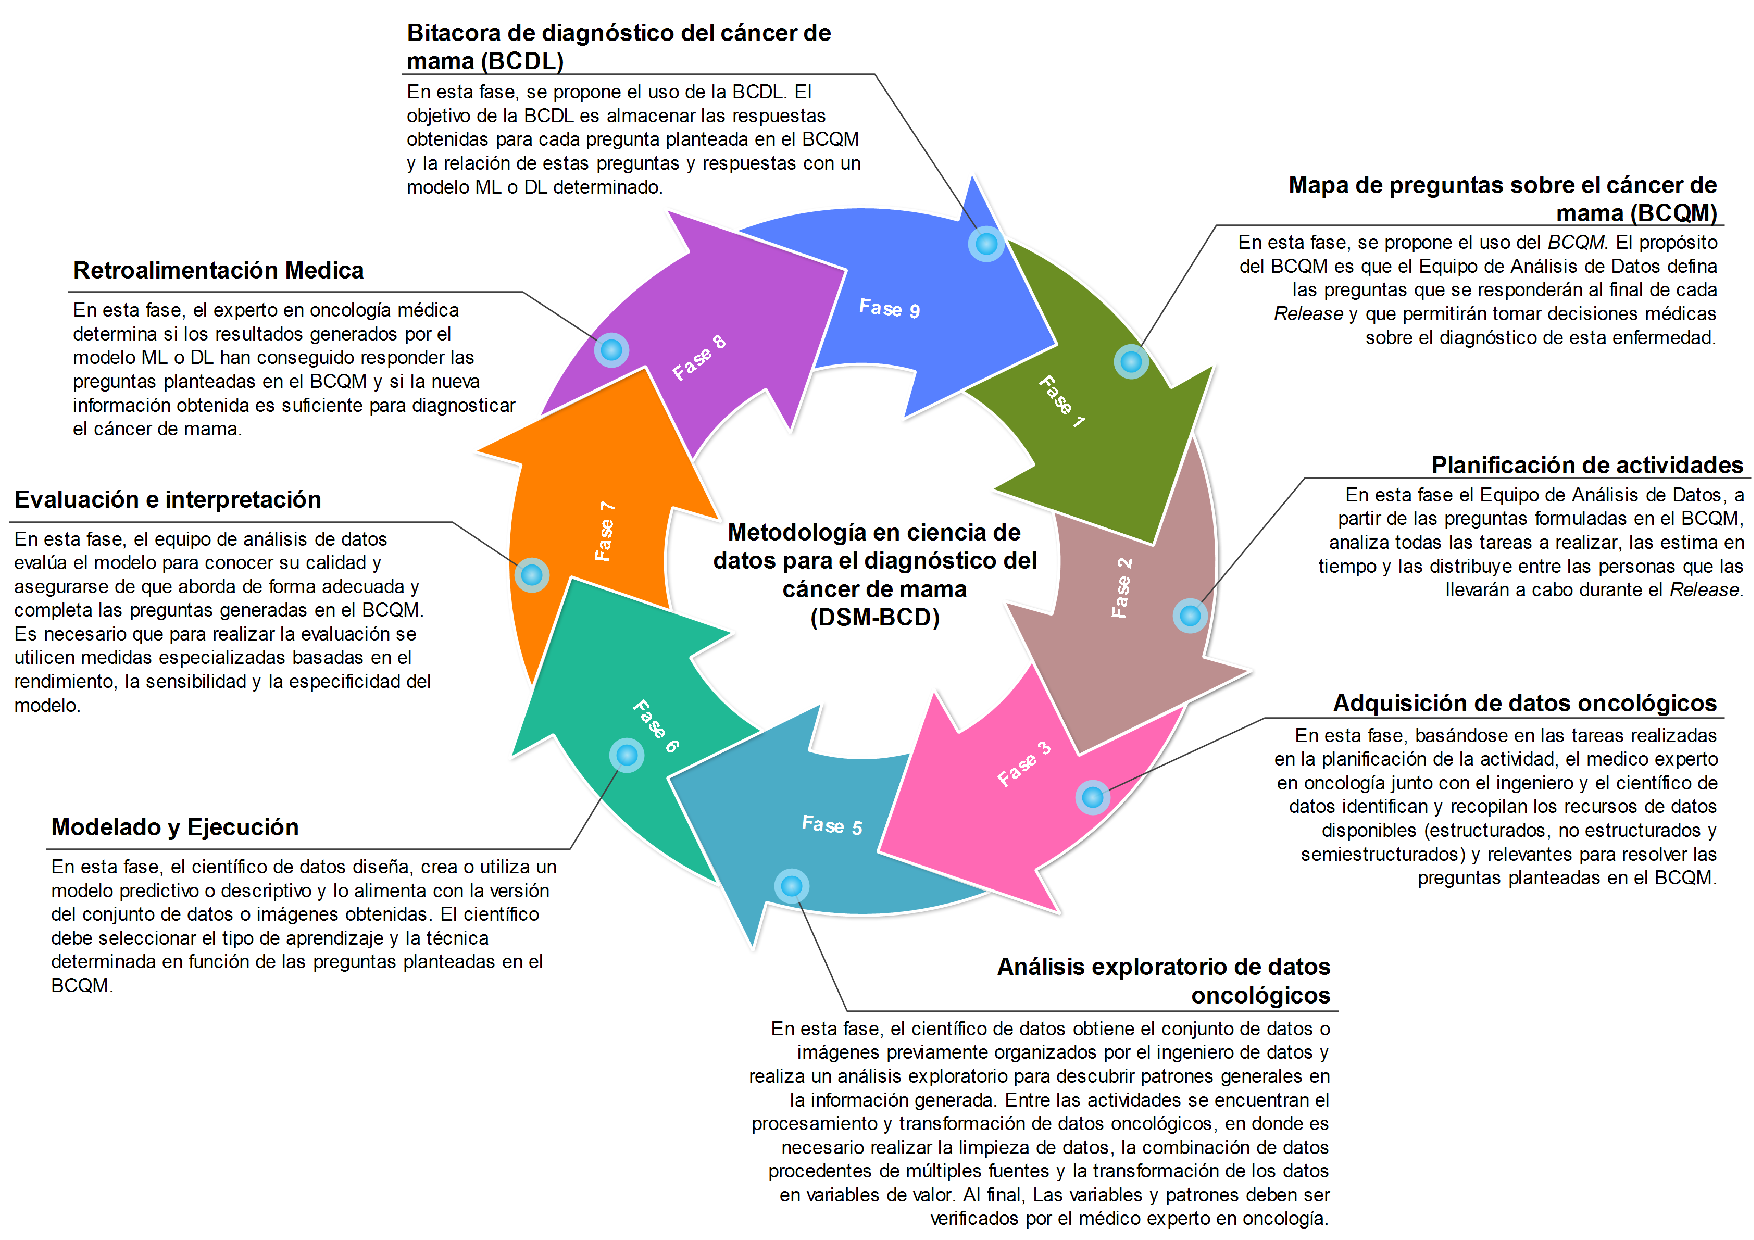
\includegraphics[width=0.9
	\linewidth]{IMAGENES/DSM-BCD_SPANISH.pdf}
	\caption{Metodología en ciencia de datos para el diagnóstico del cáncer de mama 
		(DSM-BCD)}
	\label{DSM-BCD}
\end{figure*}

Esta metodología tiene como base el \textit{manifestó ágil} aplicado a un contexto de resultados basados en datos. Dado lo anterior \textit{DSM-BCD} no se enfoca en evaluar la precisión de las técnicas de ML y DL sino su objetivo principal es generar valor a los datos en el tiempo mas corto posible para que los médicos diagnostiquen de manera ágil el cáncer de mama. Para lograrlo \textit{DSM-BCD} integra la perspicacia medica y los resultados obtenidos por las técnicas de ML y DL en una retroalimentación continua generada en cada \textit{Release} para producir mayor eficacia en la toma de decisiones

 En \textit{DSM-BCD}, se propone la conformación de un \textit{Data Analysis Team}. Este equipo debe estar encabezado por el medico experto en oncología, al menos un ingeniero de datos y un científico de datos. Se recomienda que el equipo este conformado por un máximo de 5 personas para facilitar el trabajo en equipo y la comunicación interna.
 
 Para comprender mejor el uso de DSM-BCD, se realizó un análisis descriptivo basados en datos genéticos característicos de tumores generados por los tipos de cáncer \textit{Carcinoma ductal invasivo (IDC)} y \textit{Carcinoma lobulillar invasivo (LBC)}, en donde se logró determinar que el IDC y LBC son enfermedades molecularmente distintas con rasgos genéticos característicos, lo que proporciona información importante para la estratificación de los pacientes permitiendo realizar diagnostico clínico ágil con precedentes para un tratamiento puntual.


\section{Fase 1: Mapa de preguntas sobre el cáncer de mama (BCQM)} 
En esta fase se propone el uso de un mapa de preguntas sobre el cáncer de mama (BCQM). El proposito del \textit{BCQM} es que el \textit{Data Analysis Team} defina las preguntas que serán resueltas al finalizar cada \textit{Release} y que permitirán tomar decisiones medicas con respecto al diagnostico de esta enfermedad. En la figura \ref{BCQM} se observa la estructura del BCQM.

\begin{figure}
	\centering
	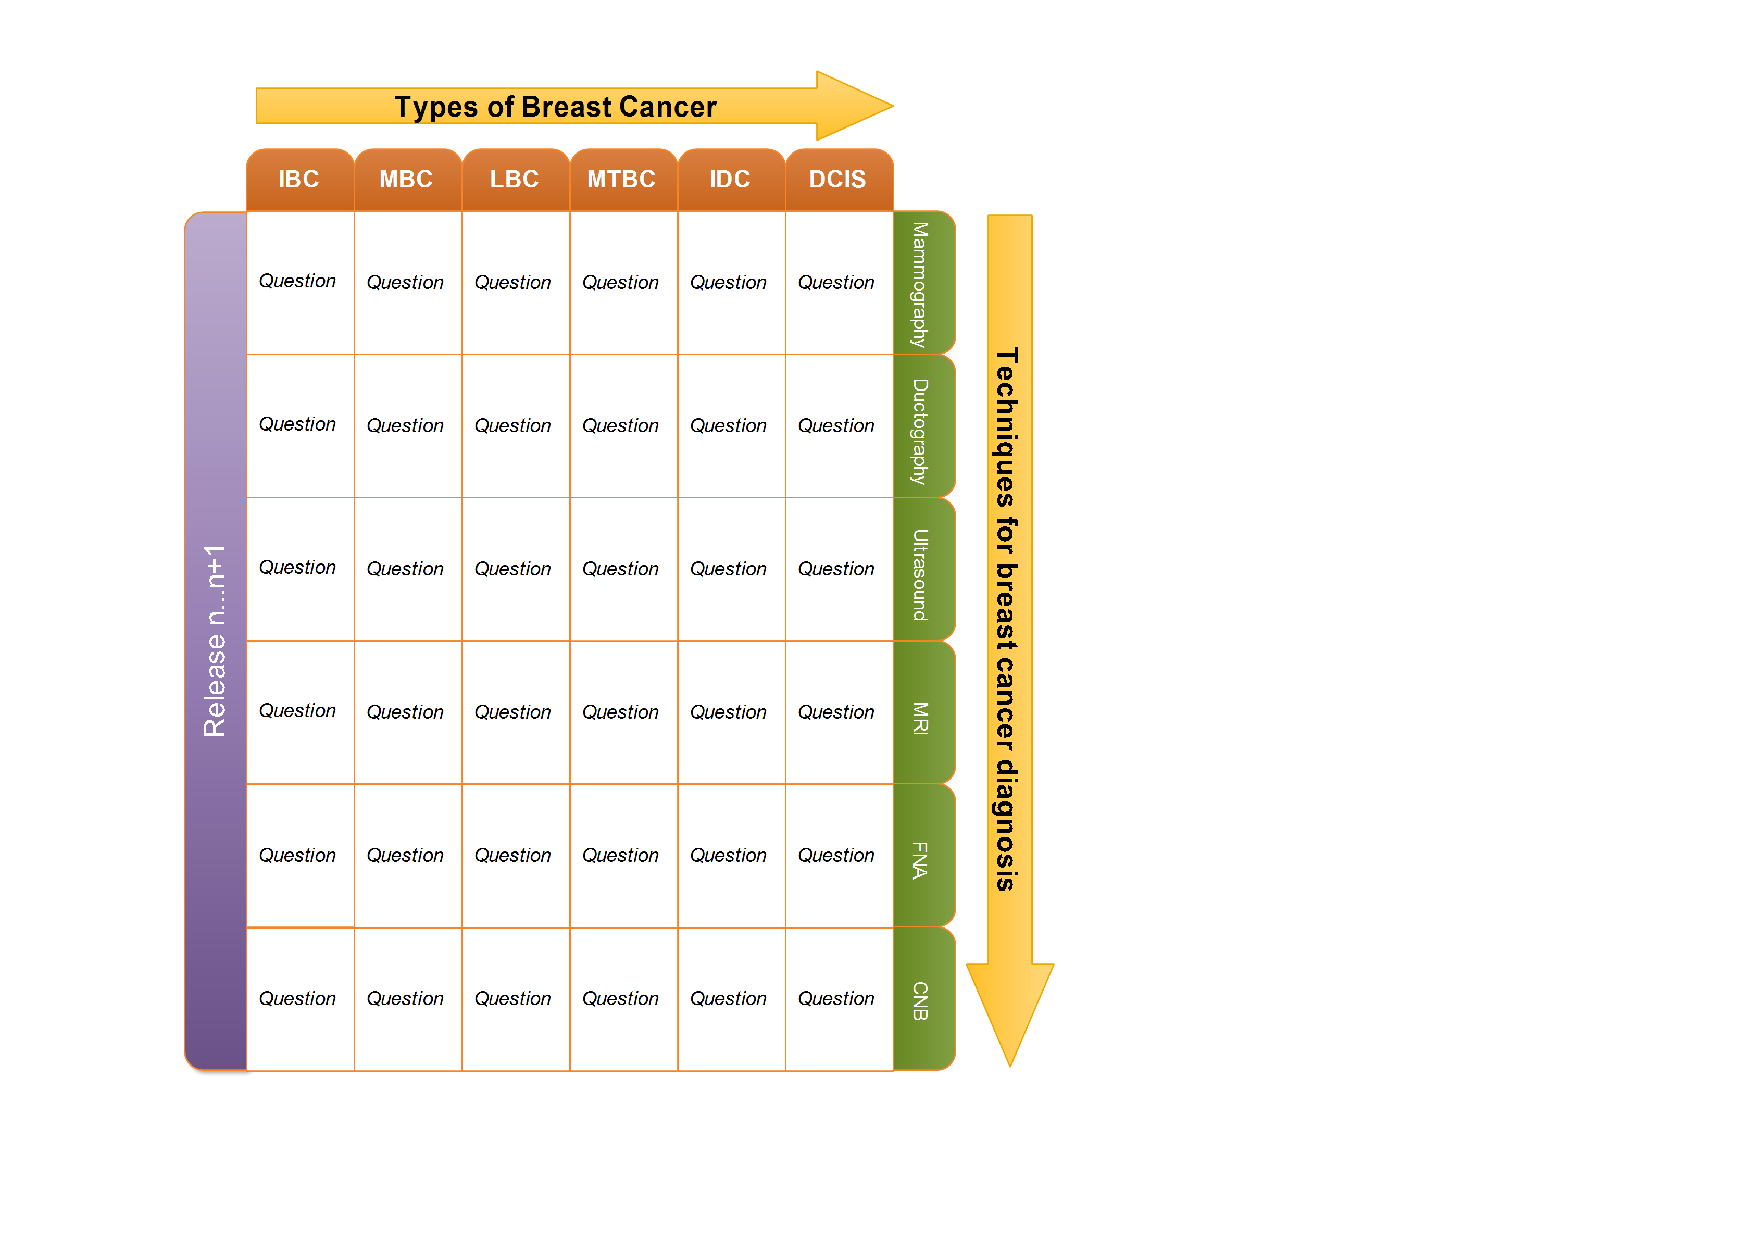
\includegraphics[width=0.6
	\linewidth]{IMAGENES/BCQM}
	\caption{Mapa de preguntas basados en los tipos de cáncer de mama \textit{inflamatorio (IBC)}, \textit{mucinoso (MBC)}, \textit{Lobulillar (LBC)}, \textit{Tumores mixtos (MTBC)}, \textit{Carcinoma ductal invasivo (IDC)} y \textit{Carcinoma ductal in situ (DCIS)}}
	\label{BCQM}
\end{figure}

El BCQM permite plantear preguntas relacionadas a los tipos de cáncer de mama y a las técnicas para el diagnostico de la misma. De modo que al finalizar el tiempo de cada \textit{Release}, el cual puede variar entre 1 y 4 semanas, las preguntas serán respondidas según el análisis de datos generado, y el medico podrá tomar una decisión de valor. Cabe resaltar, que es posible tener una o mas preguntas relacionadas a una técnica y a un tipo de cáncer de mama por cada \textit{Release}, razón por la cual es posible encontrar correlaciones entre las variables características de cada tipo de cáncer encontrando así patrones ocultos en los diferentes conjuntos de datos. Adicionalmente, el BCQM permite identificar a que técnica para el diagnostico de cáncer mama esta relacionada la pregunta a resolver, lo cual de antemano hace posible conocer el tipo información (imágenes o datos) y el algoritmo  ML o DL requerido para dar solución al problema. Así mismo, el BCQM permite definir desde la fase inicial el tipo de modelo predictivo o descriptivo según el enfoque analítico generado por la pregunta planteada. Sintetizando, el uso de BCQM facilita la comprensión del problema medico y permite identificar previamente la técnica, el tipo de información y enfoque que debe ser utilizado para el análisis de datos.  

\section{Fase 2: Planeación de actividades}
En esta fase el \textit{Data Analysis Team} basado en las preguntas realizadas en el BCQM analiza todas las tareas que hay que llevar a cabo, las estiman en tiempo y las distribuyen entre las personas que las van a realizar durante el \textit{Release}. Dado que el BCQM nos permite conocer de antemano el tipo de cáncer de mama y la técnica para el diagnostico de esta enfermedad, el científico de datos con ayuda del medico puede definir el origen de datos, lo cual va a permitir conocer el tipo, cantidad y peso de la información. Dado lo anterior, es recomendable que el equipo tenga al menos un ingeniero datos, ya que el es el encargado de tomar los datos y convertirlos en información significativa para que el científico pueda realizar el respectivo análisis.   

\section{Fase 3: Adquisición de datos oncológicos}
En esta fase, con base a la tareas realizadas en la planeación de actividades, el medico experto en oncología junto con el ingeniero y el científico de datos identifican y reúnen los recursos de datos disponibles (estructurados, no estructurados y semiestructurados) y relevantes para solucionar las preguntas planteadas en el \textit{BCQM}. Cabe resaltar, que en la metodología \textit{\textit{DSM-BCD}} es factible tener varios conjuntos de datos o imágenes que están relacionados a un tipo de cáncer de mama y una técnica de diagnostico, por lo tanto  el \textit{Data Analysis Team} puede tener a varios científicos respondiendo preguntas diferentes en un mismo \textit{Release}. Como consecuencia, al final se pueden obtener como resultado múltiples respuestas y una posible correlación entre las diversas variables oncológicas.  Asimismo, en esta fase el \textit{Data Analysis Team} debe definir la infraestructura de datos necesaria según la cantidad de información a procesar, lo cual permitirá proyectar la escalabilidad, alcance y distribución de dicha información. 

Para este caso de estudio, se utilizaron variables genéticas características de marcadores tumorales  basados en los siguientes tipos de cáncer de mama:

\begin{itemize}
	\item \textit{Carcinoma ductal invasivo (IDC)}:  Este tipo de cáncer ocurre cuando las células anormales de la mama se diseminan por todos los tejidos mamarios.
	
	\item \textit{Carcinoma lobulillar invasivo (LBC)}: Este tipo de cáncer ocurre cuando las células anormales de la mama se diseminan en lóbulo mamario.
\end{itemize}

Estas variables fueron obtenidas del conjunto de datos denominado \textit{“Breast Invasive Carcinoma (TCGA, Cell 2015)”} creado a partir del proyecto de carcinoma invasivo de mama \textit{Comprehensive Molecular Portraits of InvasiveLobular Breast Cancer} \cite{Ciriello2015} basado en el \textit {Atlas del Genoma del Cáncer (TCGA\footnote{Acrónimo de “The Cancer Genome Atlas (TCGA)”, en inglés })} cuya finalidad es catalogar cambios moleculares de importancia biológica responsables de la aparición de cáncer haciendo uso de la secuenciación genómica y la bioinformática \cite{TCGA2023}. Los datos fueron descargados del sitio público \textit{cBioPortal} para la genómica del cáncer  (\url{https://www.cbioportal.org/study/summary?id=brca_tcga_pub2015}). Cabe resaltar, que el conjunto de datos contiene un total de 817 muestras de tumores de mama que  se perfilaron con 6 plataformas moleculares: Análisis del número de copias somáticas basado en array, Secuenciación del exoma completo, perfil de metilación del ADN basado en array, secuenciación del ARN mensajero, secuenciación de microARN (miARN) y array de proteínas en fase inversa (RPPA), como se ha descrito previamente en \cite{Bass2014}. Un comité de patología revisó y clasificó todos los tumores en 490 IDC, 127 LBC, 88 casos con características mixtas de IDC e LBC, y 112 con otras histologías.

Este conjunto de datos consta de un tamaño de $818$ filas y $110$ columnas. Las variables se describen en la tabla \ref{brca_tcga_pub2015_clinical_data}: 

\begin{table*} [!htb]
	\footnotesize
	\begin{threeparttable}
		\caption{Conjunto de datos del Carcinoma invasivo de mama (TCGA, Cell 2015).}
		\label{brca_tcga_pub2015_clinical_data}
		\begin{tabular}{p{1cm} p{4cm} p{10cm}} \toprule	
			\begin{center}$N$\end{center}   
			&\begin{center}Variable\end{center}             
			&\begin{center}Descripción\end{center}      
			\\ \hline	
			%-----------------------------------------------------------------------------------
			1
			&Study ID
			&Código de identificación del estudio.
			\\ \hline
			%-----------------------------------------------------------------------------------
			2
			&Patient ID
			&Código de identificación del paciente.
			\\ \hline
			%-----------------------------------------------------------------------------------
			3
			&Sample ID
			&Código de identificación de la muestra.
			\\ \hline
			%-----------------------------------------------------------------------------------
			4
			&Diagnosis Age
			&Edad a la que se diagnosticó por primera vez una afección o enfermedad.
			\\ \hline
			%-----------------------------------------------------------------------------------
			5
			&American Joint Committee on Cancer Metastasis Stage Code
			&Código para representar la ausencia o presencia definida de diseminación a distancia o metástasis (M) a localizaciones a través de canales vasculares o linfáticos más allá de los ganglios linfáticos regionales, utilizando los criterios establecidos por el Comité Conjunto Americano del Cáncer (AJCC).
			\\ \hline
			%-----------------------------------------------------------------------------------
			6
			&Neoplasm Disease Lymph Node Stage American Joint Committee on Cancer Code
			&Los códigos que representan el estadio del cáncer en función de los ganglios presentes (estadio N) según criterios basados en múltiples ediciones del Manual de Estadificación del Cáncer de la AJCC.
			\\ \hline
			%-----------------------------------------------------------------------------------
			7
			&Neoplasm Disease Stage American Joint Committee on Cancer Code
			&La extensión de un cáncer, especialmente si la enfermedad se ha propagado desde el lugar original a otras partes del cuerpo según los criterios de estadificación de la AJCC.
			\\ \hline
			%-----------------------------------------------------------------------------------
			8
			&American Joint Committee on Cancer Publication Version Type
			&Versión o edición del American Joint Committee on Cancer Cancer Staging Handbooks, publicación del grupo formado con el propósito de desarrollar un sistema de estadificación clínica del cáncer que sea aceptable para la profesión médica estadounidense y compatible con otras clasificaciones aceptadas.
			\\ \hline
			%-----------------------------------------------------------------------------------
			9
			&American Joint Committee on Cancer Tumor Stage Code
			&Código de T patológico (tumor primario) para definir el tamaño o la extensión contigua del tumor primario (T), utilizando los criterios de estadificación del AJCC.
			\\ \hline
			%-----------------------------------------------------------------------------------
			10
			&Brachytherapy first reference point administered total dose
			&Primer punto de referencia dosis total administrada en la Braquiterapia .
			\\ \hline
		\end{tabular}
	\end{threeparttable}
\end{table*}

\section{Fase 4: Análisis Exploratorio de datos oncológicos}

En esta fase, el científico obtiene el conjunto de datos o imágenes que fueron organizados previamente por el ingeniero y realiza un \textit{Análisis exploratorio de datos} para descubrir patrones generales en la información generada. Cabe resaltar, que en esta fase el acompañamiento del medico experto en oncología es de vital importancia, ya que los datos o imágenes que van ser explorados por el científico pueden contener variables que pueden tener o no un valor significativo para el experto, ayudando así a determinar si el análisis planteado para responder la pregunta va o no por un buen camino, de modo que es posible que se agreguen o eliminen diversas variables para lograr el resultado esperado. Adicionalmente, es necesario que los diversos análisis generados estén apoyados con gráficas que sean entendibles por todo el \textit{Data Analysis Team}, esto con el proposito de aportar ideas, y desde esta fase ir encontrando posibles correlaciones entre las variables oncológicas.

\section{Fase 5: Procesamiento y transformación de datos oncológicos}
En esta fase, se abarcan todas las actividades para construir el conjunto de datos o imágenes que se utilizará en la siguiente etapa de modelado y ejecución. Entre las actividades del procesamiento y transformación de datos oncológicos, están la limpieza de datos, combinar datos de múltiples fuentes y transformar los datos en variables de valor. En esta fase, es importante el trabajo en equipo y la comunicación continua entre el ingeniero y el científico de datos para tratar los valores no válidos o faltantes, eliminar duplicados, dar un formato adecuado y combinar archivos, tablas y plataformas. Adicionalmente, el medico experto en oncología deberá proporcionar un visto bueno para proceder con la siguiente fase. Esto dado que al ser experto en el tema de dominio tiene un conocimiento mas profundo de las variables o imágenes que esta observando, y si existiese información innecesaria para el diagnostico del cáncer de mama es posible depurar dicha información para que no afecte el entrenamiento y posterior ejecución del modelo de ML y DL.

\section{Fase 6: Modelado y Ejecución}
En esta fase, el científico de datos diseña, crea o utiliza un modelo predictivo o descriptivo y lo alimenta con la versión del conjunto de datos o imágenes obtenidos en la fase de procesamiento y transformación. En esta fase, el científico debe seleccionar el tipo de aprendizaje (supervisado, no supervisado y por refuerzo) y la técnica determinada (regresión, clasificación, clustering, CNN, RNN, etc.) acorde a las preguntas planteadas en el \textit{BCQM}. Hay que mencionar que en esta fase el \textit{Data Analysis Team} debe definir junto al medico experto en oncología la tolerancia de error permitida en el modelo, esto dado a que la sensibilidad de los análisis puede variar dependiendo del tipo de cáncer de mama y la técnica de diagnostico. Es probable que el científico de datos pruebe múltiples algoritmos con sus respectivos parámetros para encontrar el mejor modelo para las variables oncológicas disponibles. Cabe resaltar, que es de vital importancia que los modelos propuestos no tengan problemas de sobre-ajuste o infra-ajuste ya que esto puede generar resultados erróneos o poco significativos. Adicionalmente, el científico de datos en cuestión junto al \textit{Data Analysis Team} deben definir la infraestructura a nivel de servidor necesaria para el entrenamiento y prueba del modelo según la cantidad de información a procesar, esto con el proposito de generar resultados acertados en el menor tiempo posible en pro de cumplir las tareas definidas en la fase de planeación de actividades y dar valor a los datos oncológicos una vez finalice el \textit{Release}.

\section{Fase 7: Evaluación e Interpretación}
En esta fase, el \textit{Data Analysis Team} evalúa el modelo para comprender su calidad y garantizar que este aborda las preguntas generadas en el \textit{BCQM} de manera adecuada y completa. Es necesario que para realizar la evaluación se utilicen medidas especializadas basadas en el rendimiento, sensibilidad y especificidad del modelo. Adicionalmente, los resultados obtenidos deben ser entendibles por el medico experto en oncología, en donde se garantice que dichos resultados sean interpretados correctamente y estén relacionados a la estadificación y los biomarcadores del cáncer de mama. Es importante que el medico junto al científico de datos ajusten el modelo según las necesidades. Dado que se esta trabajando con datos médicos sensibles, es necesario que al modelo final se aplique a un conjunto de validación para realizar una evaluación final. Además, el \textit{Data Analysis Team} puede asignar al modelo pruebas de \textit{significancia estadística} como prueba adicional para comprobar la respuesta obtenida a la pregunta generada. Esta prueba adicional es fundamental para justificar la implementación del modelo. Finalmente, dado que en el \textit{BCQM} se pueden plantear múltiples preguntas relacionadas a diferentes tipo de cáncer de mama y técnicas de diagnostico durante el \textit{Release}, es necesario que los científicos con ayuda del ingeniero de datos unan, si es posible, los resultados obtenidos en una matriz o mapa de calor para identificar el coeficiente de correlación entre dos o mas variables oncológicas. Esta matriz resultante debe ser analizada por el medico experto en oncología para determinar si existe una relación significativa entre los diferentes tipos de cáncer de mama.

\section{Fase 8: Retroalimentación medica }
En esta fase, el medico experto en oncología determina si los resultados generados por el modelo de ML o DL lograron responder las preguntas planteadas en el \textit{BCQM} y si la nueva informacion obtenida es suficiente para diagnosticar el cáncer de mama o si dichos resultados generaron información relevante para determinar la causa u origen de esta enfermedad, en pocas palabras, si los datos analizados produjeron un valor agregado al dominio medico. En el caso de que los resultados obtenidos no lograsen dar valor a los datos, el \textit{Data Analysis Team} deberá decidir si es necesario re-plantear las preguntas o si se debe adquirir nuevos datos para ajustar el modelo generado. Ademas, el experto en compañía del científico y el ingeniero de datos, basado en su perspicacia medica, deberá ayudar a decidir cual estrategia es las mas apropiada para generar resultados significativos. De forma similar, si el resultado fue satisfactorio el medico debe emitir un dictamen del \textit{nivel de impacto} que tuvo la información generada por los modelos al diagnosticar el padecimiento del cáncer de mama a un determinado paciente y unas vez comprobada la informacion, junto al \textit{Data Analysis Team} alimentar un conjunto de datos con la informacion obtenida de los diagnósticos generados a cada individuo. Lo anterior con el proposito de mejorar el desempeño de los modelos existentes y aumentar su precisión. Finalmente, en cada \textit{Release} se debe garantizar que el tiempo de diagnostico sea cada vez menor o que se genere nueva información que el medico pueda utilizar en sus funciones diarias y que ayude a determinar el origen, relación o posible tratamiento de esta enfermedad.

\section{Fase 9: Bitácora para el diagnostico del cáncer de mama (BCDL) }
En esta fase, se propone el uso de una bitácora para el diagnostico del cáncer de mama (BCDL). El proposito del \textit{BCDL} es almacenar la respuestas obtenidas por cada pregunta planteada en el \textit{BCQM} y la relación de estas preguntas y respuestas con determinado modelo de ML o DL. Esta bitácora solamente debe ser alimentada cuando la informacion obtenida generó valor agregado al dominio medico. Su principal proposito es evitar la redundancia de la informacion y la duplicidad de preguntas planteadas en el \textit{BCQM}, garantizando que en cada \textit{Release} se genere nuevo conocimiento relacionado al cáncer de mama. Se recomienda que la bitácora sea diseñada por medio de un \textit{modelo entidad relación (MER)} que este conformado por entidades como: modelo, tipo de cáncer de mama, técnica de diagnostico, conjunto de datos, pregunta y respuesta. Dado lo anterior, se sugiere que  los diferentes conjuntos de datos o imágenes utilizados en los análisis realizados, sean almacenados en un servicio de alojamiento de informacion en la nube (Amazon Cloud, Google Drive, One Drive, etc.) y que dicho informacion este identificada con un código único que facilite su búsqueda cuando sea requerido. De igual manera, los diferentes algoritmos generados deben ser almacenados en un sistema de control de versiones (GitLab, GitHub, Bitbucket, etc.) con su respectivo \textit{Readme} de funcionamiento y un código de identificación único para que pueda ser consultado fácilmente por base de datos. Por consiguiente, el uso del \textit{BCDL} permite tener una trazabilidad detallada de los avances obtenidos en cada \textit{Release} con respecto al diagnostico del cáncer de mama, esto con el proposito de que el \textit{Data Analysis Team} tenga un punto de partida solido para innovar en nuevos modelos de ML y DL a través de la comparación  y la mejora continua de modelos existentes que lograron agregar valor a los diferentes tipos de datos oncológicos.


	
	%--------------------[III] ARQUITECTURA EMPRESARIAL----------------
	\part{ARQUITECTURA Y DISEÑO}
	\chapter{Organización Empresarial}
La estructura organizativa planteada para el proyecto de investigación está basada de forma ideal en el \textit{Área de Investigación de análisis de datos} de un \textit{Instituto de Cancerología}. 

\section{Misión}
Somos una institución que trabaja por el control integral del cáncer a través de la atención y el cuidado de pacientes, la investigación, la formación de talento humano y el desarrollo de acciones en salud pública.

\section{Visión}
En 2026 el Instituto de Cancerología será referente por sus logros en la reducción de la mortalidad por cáncer, sobre la base de la innovación y la tecnología, con un actuar ético y sostenible y con un talento humano motivado y
comprometido.
\newpage

\section{Objetivo}
La investigación en su formulación y desarrollo genera dudas o problemas de carácter estadístico que necesitan un enfoque experto. El  Área de Investigación de Análisis de datos tiene por objetivo dar soporte a los investigadores de la Subdirección de Investigaciones, otras Subdirecciones y demás unidades funcionales del Instituto de Cancerología, en métodos para el manejo y análisis de datos, a través de las siguientes actividades:

\begin{itemize}
\item Proponer e implementar estrategias que permitan mantener una calidad elevada en el análisis de datos de los proyectos de investigación de la Subdirección de Investigaciones, otras Subdirecciones y demás unidades funcionales del Instituto de Cancerología.
\item Apoyar el diseño de base de datos y el desarrollo de soluciones informáticas para la captura de información de  los proyectos de investigación  y otros proyectos del Instituto de Cancerología.
\item Administrar las bases de datos de los proyectos de investigación desarrollados por el Instituto de Cancerología.
\item Desarrollar soluciones informáticas que permitan la sistematización de los diferentes procesos relacionados con la gestión y análisis de datos resultado de proyectos de investigación u otros proyectos del Instituto de Cancerología.
\item Apoyar, desde el punto de vista estadístico, la formulación de proyectos de investigación.
\item Elaborar e implementar el plan de análisis estadístico de los proyectos de investigación.
\item Apoyar los procesos de publicación científica en el componente de análisis de datos.
\item Proponer e implementar mecanismos que permitan hacer seguimiento a la ejecución de proyectos de investigación.
\item Desarrollar  modelos de simulación para estudios de evaluación económica.
\item Desarrollar modelos de simulación para la toma de decisiones en salud.
\end{itemize}

\newpage
\section{Actores,Roles y Funciones}
Los actores, Roles y funciones que conforman La jerarquía del \textit{Área de Investigación de análisis de datos} puede ser observada en la Figura\ref{organigrama}

\begin{center}
\begin{figure}[h!]
	\centering
	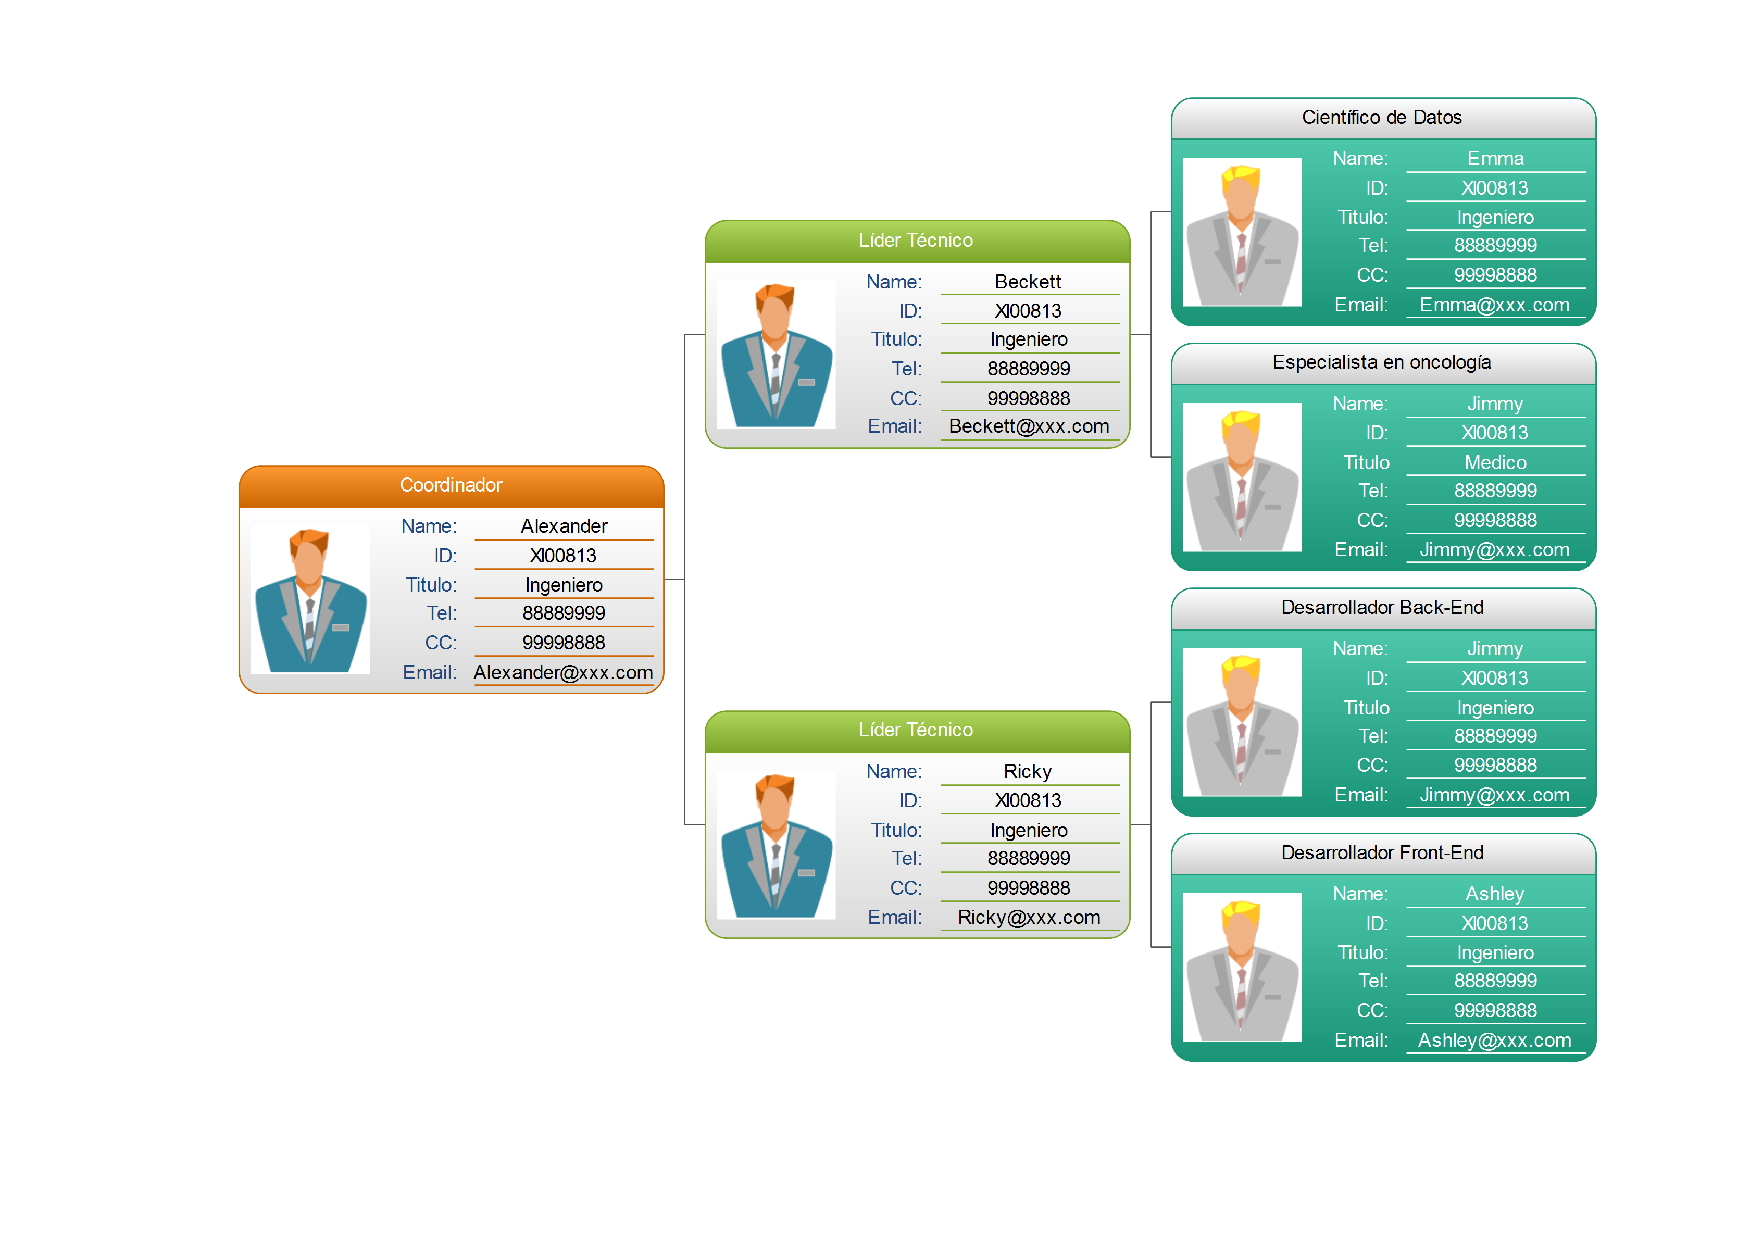
\includegraphics[width=1\linewidth]{ARQUITECTURA/imgs/organizacion}
	\caption{Jerarquía del  Área de Investigación de análisis de datos}
	\label{organigrama}
\end{figure}
\end{center}
\newpage
\section{Servicios}
El grupo de análisis de datos ofrece los siguientes servicios:
\begin{itemize}
	\item Desarrollo de modelos de decisión (árboles de decisión, modelos de Markov, simulación de eventos discretos y simulación dinámica).
	\item Desarrollo de modelos estadísticos predictivos y explicativos.
	\item Análisis de datos avanzados (modelos lineales generalizados, análisis multinivel, etc.).
	\item Análisis bioinformáticas.
	\item Estadística espacial.
	\item Minería de datos.
	\item Diseños de formularios para la captura electrónica de información (web, escritorio, apps, etc.).
	\item Administración de bases de datos.
	\item Elaboración de proyectos de investigación (métodos).
	\item Programación en R, SAS, SPSS, Stata.
	\item Evaluación económica
\end{itemize}



	\chapter{Capa de Motivación}
\section{Introducción}

Esta capa retoma, en primer lugar, algunos de los conceptos utilizados en la capa de negocio como por ejemplo el concepto de rol representado en esta capa como un Interesado (StakeHolder) y el concepto de servicio el cual tiene como equivalente un Objetivo(Goal)\cite{BolanosCastro2019}.

Es importante entender el uso e interacción de los elementos que definen la estructura de la organización, durante el proceso de apropiación de conceptos que se presenta en esta capa, se destacan los diferentes aspectos motivacionales que denotan principalmente aspectos organizacionales, en términos de cada una de las entidades encontradas y sus interacciones. Entidades como objetivos y principios que
determinan de forma detallada aspectos fundamentales de la estructura organizacional (objetivos, plan estratégico, misión y visión)\cite{BolanosCastro2019}.

Por otra parte, es importante resaltar que, dentro de la estructura organizacional un aspecto clave corresponde a las relaciones que se presentan entre los diferentes elementos. A nivel externo (principios, interesados) e interno (objetivos, requerimientos) de la organización se pueden ver estas interacciones que representan los diferentes servicios ofrecidos, mencionando sus detalles a través de requerimientos y restricciones, y también los diferentes roles que interactúan en este escenario (interesados, manejador)determinando así la comunicación entre los conceptos organizacionales \cite{BolanosCastro2019}. 

A continuación se presentan cada uno de los puntos de vista de la capa de Motivación  a partir del soporte realizado por el Área de Investigación de Análisis de datos a los investigadores de la Subdirección de Investigaciones, otras Subdirecciones y demás unidades funcionales del Instituto de Cancerología.

%-------------Punto de Vista de la Infraestructura----------%
\newpage
\section{Punto de Vista de Interesados}
El Punto de Vista de Interesados permite al analista modelar las partes interesadas, los impulsores internos y externos del cambio y las evaluaciones en términos de fortalezas, debilidades, oportunidades y amenazas de dichos controladores . Ademas,se pueden describir los vínculos con los objetivos iniciales de alto nivel que abordan estas preocupaciones y evaluaciones. Estos objetivos forman la base para el proceso de ingeniería de requisitos, incluyendo refinamiento de objetivos, contribucion y análisis de conflictos, y la derivación de requisitos que realicen las metas\cite{BolanosCastro2019}.

En la Figura \ref{PvInteresados}, se plantea el Caso para el Punto de Vista de Interesados con cada uno de los elementos que interactúan entre sí. 

\begin{figure}[h!]
	\centering
	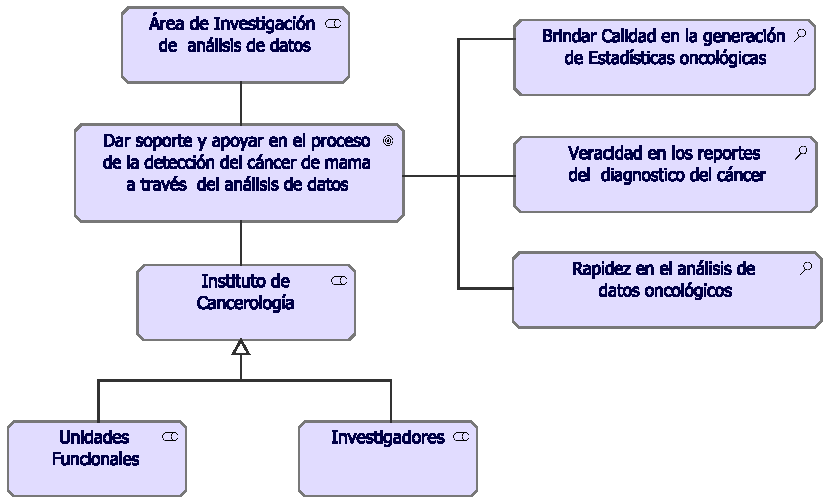
\includegraphics[width=1\linewidth]{ARQUITECTURA/imgs/CapaMotivacion/1_PvInteresados}
	\caption{Punto de Vista de Interesados}
	\label{PvInteresados}
\end{figure}

\begin{enumerate}[label=\textbf{\arabic*})]
	

\item  \textbf{Área de Investigación de análisis de datos:} Corresponde a una de las dependencias del área de investigación la cual  tiene por objetivo dar soporte a los investigadores de la Subdirección de Investigaciones, otras Subdirecciones y demás unidades funcionales del Instituto de Cancerología, haciendo uso métodos computacionales para el manejo y análisis de datos Oncológicos.
	
\item  \textbf{Dar soporte y apoyar en el proceso de la detección del cáncer de mama a través del análisis de datos:} Este objetivo organizacional hace referencia a el servicio de generar diagnósticos relacionados con el cáncer de mama  solicitados por los diferentes funcionarios del Instituto de Cancerología.Se asocia con dos Stakeholder: \textit{Área de Investigación de análisis de datos} e \textit{Instituto de Cancerología}; el primero es el que vela por el cumplimiento del objetivo;el segundo es a quien se brinda el servicio del Diagnostico del Cáncer de mama. 

\item  \textbf{Instituto de Cancerología:} Este rol de aplicación corresponde a los diferentes usuarios del instituto de nacional de cancerología. Tienes asociado el actor \textit{Investigadores} y el actor \textit{Unidades funcionales }. Estos roles se describen a continuación: 
\begin{itemize}
	\item  \textbf{\textit{Investigadores:}}  Este rol está conformado por todos los grupos de investigación en cáncer del país registrados ante Colciencias y adicionalmente, con representantes de diferentes tipos de usuarios del conocimiento generado por la investigación como son las sociedades médicas, los prestadores de servicios oncológicos, los aseguradores, las autoridades sanitarias y los pacientes entre otros. 
	
	\item  \textbf{\textit{Unidades Funcionales :}}  Este rol está conformado por las unidades clínicas ubicadas al interior del Instituto de Cancerología cuya función es evaluar la situación de salud del paciente con diagnóstico presuntivo de cáncer. 
\end{itemize}

\item  \textbf{Brindar Calidad en la generación de Estadísticas Oncológicas:} Teniendo en cuenta el objetivo \textit{Dar soporte y apoyar en el proceso de la detección del cáncer de mama a través del análisis de datos}, se tiene esta valoración. En este caso, el resultado es la oportunidad de generar calidad en la información estadística acerca de la identificación del cáncer de mama diversos pacientes.

\item  \textbf{Veracidad en los reportes del diagnostico:} Teniendo en cuenta el objetivo \textit{Dar soporte y apoyar en el proceso de la detección del cáncer de mama a través del análisis de datos}, se tiene esta valoración. En este caso, el resultado es la oportunidad de generar diagnósticos exactos acerca de las posibilidad de padecer cáncer de mama.  

\item  \textbf{Rapidez en el análisis de datos oncológicos:} Teniendo en cuenta el objetivo \textit{Dar soporte y apoyar en el proceso de la detección del cáncer de mama a través del análisis de datos}, se tiene esta valoración. En este caso, el resultado es la oportunidad de generar de forma eficiente diversos reportes enfocados en el diagnostico de cáncer de mama en el menor tiempo posible para poder dar un tratamiento oportuno a cada paciente.
\end{enumerate}

%-------------Punto de Vista de Realización de Objetivos----------%
\newpage
\section{Punto de Vista de Realización de Objetivos}
El Punto de Vista de Realización de Objetivos permite modelar el refinamiento de metas (de alto nivel) en metas más concretas y el refinamiento de objetivos concretos en requisitos o restricciones que describen las propiedades que se necesitan para realizar las metas\cite{BolanosCastro2019}. 

En la Figura \ref{PvRealizacionObj}, se plantea el Caso para el Punto de Vista de Realización de Objetivos con cada uno de los elementos que interactúan entre sí. 

\begin{figure}[h!]
	\centering
	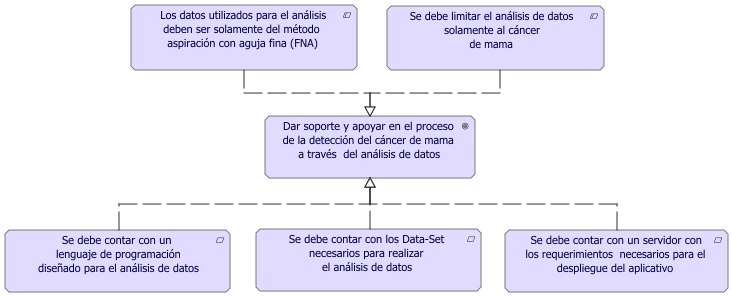
\includegraphics[width=1\linewidth]{ARQUITECTURA/imgs/CapaMotivacion/2_PvRealizacionObj}
	\caption{Punto de Vista de Realización de Objetivos}
	\label{PvRealizacionObj}
\end{figure}

\begin{enumerate}[label=\textbf{\arabic*})]
\item  \textbf{Dar soporte y apoyar en el proceso de la detección del cáncer de mama a través del análisis de datos:} el objetivo organizacional cuenta con tres requerimientos y dos restricciones. En este caso, este objetivo es el encargado de realizarlos.

\item  \textbf{Se debe contar con un lenguaje de programación diseñado para el análisis de datos:} Este requerimiento plantea que para poder generar el diagnostico de cáncer es necesario utilizar un lenguaje de programación que contenga herramientas y funcionalidades enfocados en el procesamiento y análisis de datos.

\item  \textbf{Se debe contar con los Data-Set necesarios para realizar el análisis de datos:} Este requerimiento se refiere a que los datos sobre los que se va a realizar el análisis deben contener variables de pacientes ya diagnosticados con cáncer de mama que permitan el entrenamiento de los algoritmos que clasificaran nuevos pacientes  candidatos de padecer dicho cáncer.

\newpage
\item  \textbf{Se debe contar con un servidor con los requerimientos necesarios para el despliegue del aplicativo:} Este requerimiento se refiere a que el servidor en el cual se va a desplegar el Back-End y el Front-End de la aplicación BreastApp debe contener las prestaciones de almacenamiento y procesamiento suficiente para la generación  optima de diagnósticos asociados al cáncer de mama.

\item  \textbf{Los datos utilizados para el análisis deben ser solamente del método aspiración con aguja fina (FNA):} Este restricción hace referencia a que las variables necesarias para el diagnostico de cáncer de mama deben ser solamente las obtenidas por el método FNA, esto debido a que el aplicativo esta diseñado para generar los diagnósticos con base solamente a este método.

\item  \textbf{Se debe limitar el análisis de datos solamente al cáncer de mama:} Este restricción hace referencia que el aplicativo esta enfocado solamente al cáncer de mama y no a otro tipo de cáncer. Se realiza esta limitación para que la generación de reportes sea rápida y el cáncer pueda tratarse a tiempo.
\end{enumerate}

%-------------Punto de Vista de Realización de Objetivos----------%
\newpage
\section{Punto de Vista de Contribución de Objetivos}

El Punto de Vista de Contribución de Objetivos permite a un analista modelar las relaciones de influencia entre objetivos y requisitos. Las vistas resultantes en este punto de vista pueden usarse para analizar el impacto que las metas tienen entre sí o para detectar conflictos entre los objetivos de las partes interesadas\cite{BolanosCastro2019}. 

En la Figura \ref{PvContribucionObj}, se plantea el Caso para el Punto de Vista de Contribución de Objetivos con cada uno de los elementos que interactúan entre sí. 

\begin{figure}[h!]
	\centering
	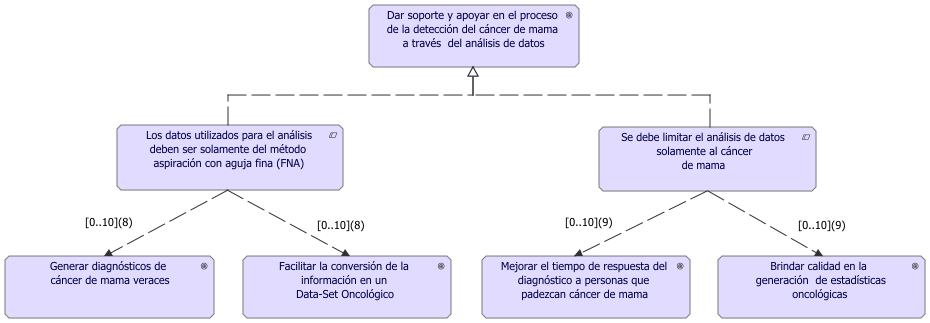
\includegraphics[width=1\linewidth]{ARQUITECTURA/imgs/CapaMotivacion/3_PvContribucionObj}
	\caption{Punto de Vista de Contribución de Objetivos}
	\label{PvContribucionObj}
\end{figure}

\begin{enumerate}[label=\textbf{\arabic*})]
	\item  \textbf{Dar soporte y apoyar en el proceso de la detección del cáncer de mama a través del análisis de datos:} para este punto de vista, se toman en cuenta las restricciones que realiza
	este objetivo organizacional, planteada en el modelo del punto de vista anterior. Esta se describe en el apartado siguiente.
	
	\item  \textbf{Los datos utilizados para el análisis deben ser solamente del método aspiración con aguja fina (FNA):} Este restricción hace referencia a que las variables necesarias para el diagnostico de cáncer de mama deben ser solamente las obtenidas por el método FNA, esto debido a que el aplicativo esta diseñado para generar los diagnósticos con base solamente a este método. Esta restricción tiene dos objetivos con impacto positivo. El impacto se mide en una escala de 1 a 10, siendo 10 el más alto y el impacto más positivo.
	
	\begin{itemize}
		\item  \textbf{\textit{Generar diagnósticos de cáncer de mama veraces:}} Teniendo en cuenta la restricción anterior se tiene un impacto positivo en este objetivo debido a que al procesar solamente datos obtenidos por el método de aguja fina(FNA) el entrenamiento de los algoritmos van a generar resultados cada vez mas precisos en la detección del cáncer de mama. El nivel de impacto asociado es de 8.
		
		\item  \textbf{\textit{Facilitar la conversión de la información en un Data-Set Oncológico:}}
		Teniendo en cuenta la restricción anterior se tiene un impacto positivo en este objetivo debido a que el método de aguja fina(FNA) es bastante utilizado en el ámbito medico,por lo que las estandarización e identificación de variables facilita la generación diversos Data-Set para el diagnostico de cáncer de mama.El nivel de impacto asociado es de 8.
	\end{itemize}
	
	\item  \textbf{Se debe limitar el análisis de datos solamente al cáncer de mama:} Este restricción hace referencia que el aplicativo esta enfocado solamente al cáncer de mama y no a otro tipo de cáncer. Se realiza esta limitación para que la generación de reportes sea rápida y el cáncer pueda tratarse a tiempo.Esta restricción tiene dos objetivos con impacto positivo. El impacto se mide en una escala de 1 a 10, siendo 10 el más alto y el impacto más positivo.
	
	\begin{itemize}
		\item  \textbf{\textit{Mejorar el tiempo de respuesta del diagnostico a personas que padecen cáncer de mama:}} Teniendo en cuenta la restricción anterior se tiene un impacto positivo debido a que al enfocarse solamente en el cáncer de mama la generación de diagnósticos es mas rápida ya que el sistema esta diseñado solamente para este tipo de cáncer.El nivel de impacto asociado es de 9.
		
		\item  \textbf{\textit{Brindar calidad en la generación de estadísticas Oncológicas:}} Teniendo en cuenta la restricción anterior se tiene un impacto positivo debido a que al enfocarse solamente en el cáncer de mama los algoritmos del sistema cada vez van a irse entrenando con una gran cantidad de datos mayor que va a garantizar cada vez un resultado mas exacto del diagnostico de cáncer de mama. 
	\end{itemize}

\end{enumerate}

%-------------Punto de Vista de Principios----------%
\newpage
\section{Punto de Vista de Principios}

El Punto de Vista de Principios permite al analista modelar los principios que son relevantes para el problema de diseño en cuestión, incluyendo los objetivos que motivan dichos principios \cite{BolanosCastro2019}. 

En la Figura \ref{PvPrincipios}, se plantea el Caso para el Punto de Vista de principios con cada uno de los elementos que interactúan entre sí. 

\begin{figure}[h!]
	\centering
	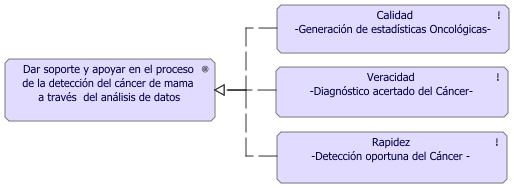
\includegraphics[width=1\linewidth]{ARQUITECTURA/imgs/CapaMotivacion/4_PvPrincipios}
	\caption{Punto de Vista de Principios}
	\label{PvPrincipios}
\end{figure}

\begin{enumerate}[label=\textbf{\arabic*})]
	\item  \textbf{Dar soporte y apoyar en el proceso de la detección del cáncer de mama a través del análisis de datos:} Este objetivo organizacional hace referencia a el servicio de generar diagnósticos relacionados con el cáncer de mama  solicitados por los diferentes funcionarios del Instituto de Cancerología.Realiza tres principios representativos para la organización, descritos a continuación.
	
	\begin{itemize}
		\item  \textbf{\textit{Calidad:}} Generación de estadísticas oncologicas con una adecuada organización para una mayor compresión y análisis.
		
		\item  \textbf{\textit{Veracidad:}} Precisión  alta en el diagnostico y detección del Cáncer de mama.
		
		\item  \textbf{\textit{Rapidez:}}  Generación de diagnósticos del cáncer de mama de forma eficiente para un tratamiento oportuno.
	\end{itemize}
\end{enumerate}

%-------------Punto de Vista Realización de Requerimientos----------%
\newpage
\section{Punto de Vista de Realización de Requerimientos }

El Punto de Vista de Realización de Requerimientos permite a los implicados modelar la realización de los requisitos por parte de los elementos básicos, como los actores empresariales y los servicios empresariales. Este punto de vista tiene en cuenta elementos como los procesos empresariales, los servicios y componentes de la aplicación. Además, puede usarse para refinar requisitos en requisitos mas detallados\cite{BolanosCastro2019}. 

En la Figura \ref{PvRealizacionReq}, se plantea el Caso para el Punto de Vista de Realización de Requerimientos con cada uno de los elementos que interactúan entre sí. 

\begin{figure}[h!]
	\centering
	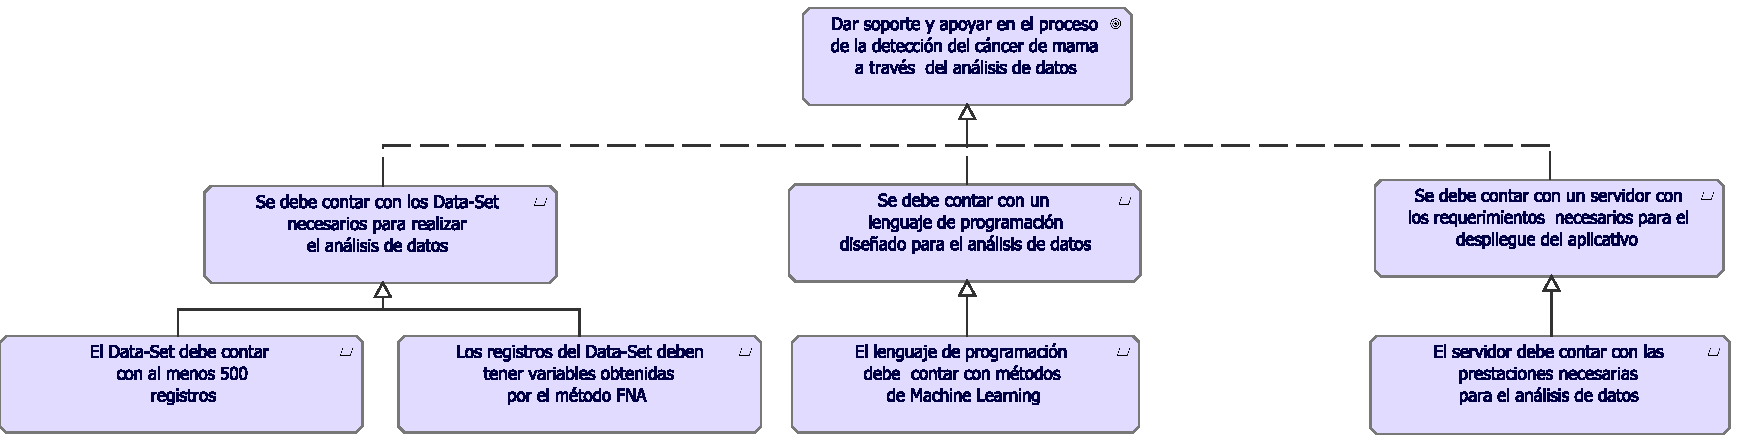
\includegraphics[width=1\linewidth]{ARQUITECTURA/imgs/CapaMotivacion/5_PvRealizacionReq}
	\caption{Punto de Vista de Realización de Requerimientos}
	\label{PvRealizacionReq}
\end{figure}

\begin{enumerate}[label=\textbf{\arabic*})]
	\item  \textbf{Dar soporte y apoyar en el proceso de la detección del cáncer de mama a través del análisis de datos:} El	objetivo organizacional cuenta con tres requerimientos. En este caso,
	este objetivo es el encargado de realizarlos.
	
	\item  \textbf{Se debe contar con un lenguaje de programación diseñado para el análisis de datos:} Este requerimiento plantea que para poder generar el diagnostico de cáncer es necesario utilizar un lenguaje de programación que contenga herramientas y funcionalidades enfocados en el procesamiento y análisis de datos. Este requerimiento tiene asociado los dos requerimientos que se detallan a continuación:
	
	\begin{itemize}
		\item  \textbf{\textit{El Data-Set debe contar con al menos 500 registros:}} Es necesario para el entrenamiento de los algoritmos de Machine Learning contar con información mayor o igual a 500 registros de pacientes los cuales incluyan las variables necesarias para el entrenamiento de dichos algoritmos para realizar posteriormente el diagnostico de nuevos pacientes.   
		
		\item  \textbf{\textit{Los registros del Data-Set deben tener variables obtenidas por el método FNA:}} Es necesario que las variables obtenidas sean del método medico de  aspiración con aguja fina (FNA) esto debido a que el aplicativo esta diseñado para generar los diagnósticos con base solamente a este método.
	\end{itemize}
	
	\item  \textbf{Se debe contar con un lenguaje de programación diseñado para el análisis de datos:} Este requerimiento plantea que para poder generar que el diagnostico de cáncer es necesario utilizar un lenguaje de programación que contenga herramientas y funcionalidades enfocados en el procesamiento y análisis de datos. Este requerimiento tiene asociado el requerimiento que se detalla a continuación:
	
	\begin{itemize}
		\item  \textbf{\textit{El lenguaje de programación debe contar con métodos de Machine Learning:}} Es necesario que el lenguaje de programación cuente con métodos de Machine Learning debido a que por medio de ellos es que se realiza el diagnostico de cáncer de mama.
	\end{itemize}
	
	\item  \textbf{Se debe contar con un servidor con los requerimientos necesarios para el despliegue del aplicativo:} Este requerimiento se refiere a que el servidor en el cual se va a desplegar el Back-End y el Front-End de la aplicación BreastApp debe contener las prestaciones de almacenamiento y procesamiento suficiente para la generación  optima de diagnósticos asociados al cáncer de mama. Este requerimiento tiene asociado el requerimiento que se detalla a continuación:
	
	\begin{itemize}
		\item  \textbf{\textit{El servidor debe contar con las	prestaciones necesarias para el análisis de datos:}} Es necesario que el servidor cuente con la memoria suficiente de almacenamiento y procesamiento  debido a que la cantidad de datos y cálculos realizados por los métodos de Machine Learning es bastante alta.
	\end{itemize}
	
\end{enumerate}

%-------------Punto de Vista de Motivación----------%
\newpage
\section{Punto de Vista de Motivación }

El Punto de Vista de Motivación permite al diseñador o analista modelar el aspecto de las razones (motivaciones), que guían el diseño o el cambio de una Arquitectura Empresarial.Este punto de vista puede utilizarse para presentar un panorama completo o parcial del aspecto de la motivación relacionando a las
partes interesadas, sus objetivos principales, los principios que se aplican y los principales requisitos de servicios, procesos, aplicaciones y objetos\cite{BolanosCastro2019}. 

En la Figura \ref{PvMotivacion}, se plantea el Caso para el Punto de Vista de Motivación con cada uno de los elementos que interactúan entre sí. 

\begin{figure}[h!]
	\centering
	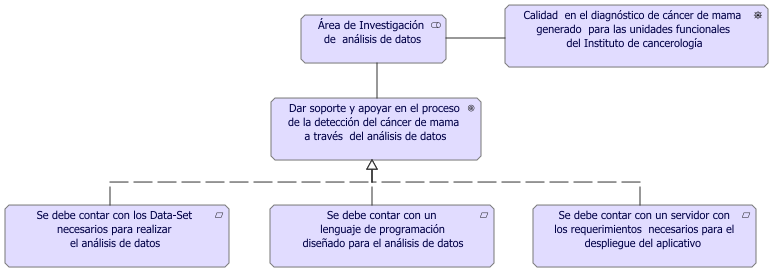
\includegraphics[width=1\linewidth]{ARQUITECTURA/imgs/CapaMotivacion/6_PvMotivacion}
	\caption{Punto de Vista de Motivación}
	\label{PvMotivacion}
\end{figure}

\begin{enumerate}[label=\textbf{\arabic*})]
	\item  \textbf{Dar soporte y apoyar en el proceso de la detección del cáncer de mama a través del análisis de datos:} El objetivo organizacional cuenta con tres requerimientos. En este caso, este objetivo es el encargado de realizarlos. Ademas, se asocia con el StakeHolder \textit{Área de Investigación de  análisis de datos}.
	
	\item  \textbf{Se debe contar con un lenguaje de programación diseñado para el análisis de datos:} Este requerimiento plantea que para poder generar el diagnostico de cáncer es necesario utilizar un lenguaje de programación que contenga herramientas y funcionalidades enfocados en el procesamiento y análisis de datos.
	
	\item  \textbf{Se debe contar con los Data-Set necesarios para realizar el análisis de datos:} Este requerimiento se refiere a que los datos sobre los que se va a realizar el análisis deben contener variables de pacientes ya diagnosticados con cáncer de mama que permitan el entrenamiento de los algoritmos que clasificaran nuevos pacientes  candidatos de padecer dicho cáncer.
	
	\item  \textbf{Se debe contar con un servidor con los requerimientos necesarios para el despliegue del aplicativo:} Este requerimiento se refiere a que el servidor en el cual se va a desplegar el Back-End y el Front-End de la aplicación BreastApp debe contener las prestaciones de almacenamiento y procesamiento suficiente para la generación  optima de diagnósticos asociados al cáncer de mama.

	\item  \textbf{Calidad  en el diagnóstico de cáncer de mama generado para las unidades funcionales del Instituto de cancerología:} Este conductor hace referencia a la búsqueda de mejoramiento en la atención a pacientes de los investigadores de la Subdirección de Investigaciones, otras Subdirecciones y demás unidades funcionales del Instituto de Cancerología con base en la generación de diagnosticos de cáncer de mama con un nivel de calidad alto .Se asocia con el StakeHolder \textit{Área de Investigación de análisis de datos}.	
\end{enumerate}



	\chapter{Capa de Estrategia}
\section{Introducción}

Esta capa plantea los aspectos estratégicos de la empresa. Cada uno de los puntos de vista que contiene esta capa presenta una perspectiva diferente sobre el modelado de la dirección estratégica de alto nivel y la composición de la organización\cite{ArchiMate3.0.1}. 

Esta capa  busca establecer y conocer los diferentes planes estratégicos que van a tomar lugar en los procesos de negocio actuales de la organización, por lo tanto, es importante tener en cuenta los conceptos utilizados en la capa de Motivación para así facilitar la identificación de los diferentes usos e interacciones que se presentan con esta capa. Para una adecuada apropiación de la conceptualización de esta capa, se implementa el uso de cuatro diferentes puntos de vista: Estrategia, Mapa de capacidad,Realización de Resultado y Mapa de recurso.

A continuación se presentan cada uno de los puntos de vista de la capa de Estrategia  a partir del soporte realizado por el Área de Investigación de Análisis de datos a los investigadores de la Subdirección de Investigaciones, otras Subdirecciones y demás unidades funcionales del Instituto de Cancerología.

%-------------Punto de Vista Estretegia----------%
\newpage
\section{Punto de Vista de la Estrategia}

El punto de vista de la estrategia permite a la organización modelar una visión general estratégica de alto nivel de los cursos de acción de la empresa, las capacidades y recursos que los respaldan, y los resultados previstos\cite{ArchiMate3.0.1}. 

En la Figura \ref{PvEstretegia} se plantea el Caso para el Punto de Vista de la Estrategia con cada uno de los elementos que interactúan entre sí. 

\begin{figure}[h!]
	\centering
	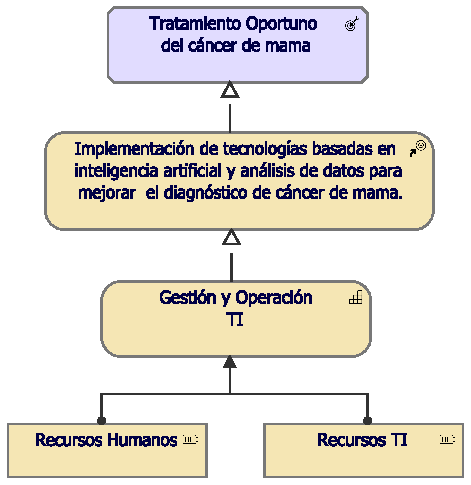
\includegraphics[width=0.75\linewidth]{ARQUITECTURA/imgs/CapaEstrategica/1_PvEstrategia}
	\caption{Punto de Vista de la Estrategia}
	\label{PvEstretegia}
\end{figure}

\begin{enumerate}[label=\textbf{\arabic*})]
	
\item  \textbf{Tratamiento Oportuno del cáncer de mama:} Hace referencia al \textit{resultado} que espera obtener el Instituto de Cancerología a través del Área de Investigación de Análisis de datos. Este resultado esta basado en la rapidez y veracidad de los diagnósticos de cáncer de mama generados para cada paciente que tiene como consecuencia un tratamiento a tiempo que permita sanar dicho cáncer.

\item  \textbf{Implementación de tecnologías basadas en  inteligencia artificial y análisis de datos para 	mejorar  el diagnóstico de cáncer de mama :} Hace referencia al \textit{curso de acción} planteado por el Instituto de Cancerología a través del Área de Investigación de Análisis de datos para obtener un \textit{Tratamiento Oportuno del cáncer de mama}.

\item  \textbf{Gestión y Operación TI:} Hace referencia a la \textit{capacidad} con respecto a la gestión y operación de Tecnologías de la Informacion del Área de Investigación de Análisis de datos para realizar el curso de acción de \textit{Implementación de tecnologías basadas en  inteligencia artificial y análisis de datos para 	mejorar  el diagnóstico de cáncer de mama}. Esta asignado a los siguientes recursos:

\begin{itemize}
	\item  \textbf{\textit{Recursos Humanos:}} Este recurso hace referencia a los coordinadores, lideres técnicos,Especialistas en Oncología, científicos de datos  y desarrolladores del Área de Investigación de Análisis de datos los cuales poseen habilidades en la gestión y operación de las Tecnologías de la Informacion.
	
	\item  \textbf{\textit{Recursos TI:}} Este recurso hace referencia a las herramientas basadas en las Tecnologías de la Informacion que influyen en la realización de diagnósticos oncológicos. En este caso la principal herramienta para la generación de diagnósticos de cáncer de mama es la aplicación web \textit{BreastApp}.
\end{itemize}
	
 \end{enumerate}

%-------------Punto de Vista Capa de Capacidad----------%
\newpage
\section{Punto de Vista del Mapa de Capacidad}

El punto de vista del mapa de capacidad permite crear una visión general estructurada de las capacidades de la empresa. Un mapa de capacidades generalmente muestra dos o tres niveles de las capacidades en toda la organización. Puede, por ejemplo, usarse como un mapa de calor para identificar áreas de inversión. En algunos casos, un mapa de capacidades también puede mostrar resultados específicos entregados por estas capacidades\cite{ArchiMate3.0.1}. 

En la Figura \ref{PvMapaCapacidad} se plantea el Caso para el Punto de Vista del Mapa de Capacidad con cada uno de los elementos que interactúan entre sí. 

\begin{figure}[h!]
	\centering
	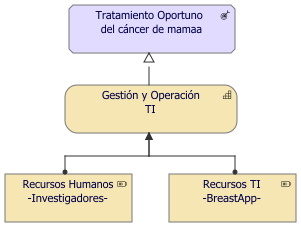
\includegraphics[width=0.75\linewidth]{ARQUITECTURA/imgs/CapaEstrategica/2_PvMapaCapacidad}
	\caption{Punto de Vista del Mapa de Capacidad}
	\label{PvMapaCapacidad}
\end{figure}

\begin{enumerate}[label=\textbf{\arabic*})]
	
\item  \textbf{Tratamiento Oportuno del cáncer de mama:} Hace referencia al \textit{resultado} que espera obtener el Instituto de Cancerología a través del Área de Investigación de Análisis de datos. Este resultado esta basado en la rapidez y veracidad de los diagnósticos de cáncer de mama generados para cada paciente que tiene como consecuencia un tratamiento a tiempo que permita sanar dicho cáncer.

\newpage
\item  \textbf{Gestión y Operación TI:} Hace referencia a la \textit{capacidad} con respecto a la gestión y operación de Tecnologías de  la Informacion del Área de Investigación de Análisis de datos para realizar el curso de acción de \textit{Implementación de tecnologías basadas en  inteligencia artificial y análisis de datos para 	mejorar  el diagnóstico de cáncer de mama}. Esta asignado a los siguientes recursos:
	
	\begin{itemize}
		\item  \textbf{\textit{Recursos Humanos:}} Este recurso hace referencia a los coordinadores, lideres técnicos,Especialistas en Oncología, científicos de datos  y desarrolladores del Área de Investigación de Análisis de datos los cuales poseen habilidades en la gestión y operación de las Tecnologías de la Informacion.
		
		\item  \textbf{\textit{Recursos TI:}} Este recurso hace referencia a las herramientas basadas en las Tecnologías de la Informacion que influyen en la realización de diagnósticos oncológicos. En este caso la principal herramienta para la generación de diagnósticos de cáncer de mama es la aplicación web \textit{BreastApp}.
	\end{itemize}
	
\end{enumerate}

%-------------Punto de Vista Capa de Capacidad----------%
\newpage
\section{Punto de Vista de la Realización de Resultado}

El punto de vista de realización del resultado se utiliza para mostrar los resultados orientados al negocio ,considerados de alto nivel, son realizados por las capacidades y los elementos centrales de la organización\cite{ArchiMate3.0.1}. 

En la Figura \ref{PvRealizacion} se plantea el Caso para el Punto de Vista de la realización de resultado con cada uno de los elementos que interactúan entre sí. 

\begin{figure}[h!]
	\centering
	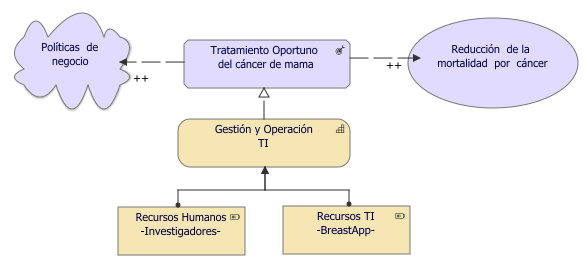
\includegraphics[width=1\linewidth]{ARQUITECTURA/imgs/CapaEstrategica/3_PvRealizacion}
	\caption{Punto de Vista de la Realización de Resultado}
	\label{PvRealizacion}
\end{figure}


\begin{enumerate}[label=\textbf{\arabic*})]
	
\item  \textbf{Tratamiento Oportuno del cáncer de mama:} Hace referencia al \textit{resultado} que espera obtener el Instituto de Cancerología a través del Área de Investigación de Análisis de datos. Este resultado esta basado en la rapidez y veracidad de los diagnósticos de cáncer de mama generados para cada paciente que tiene como consecuencia un tratamiento a tiempo que permita sanar dicho cáncer.

\item  \textbf{Políticas de negocio:} Hace referencia al elemento asociado al core del instituto de Cancerología el cual esta basado en el control integral del cáncer a través de la atención y el cuidado de pacientes, la investigación, la formación de talento humano y el desarrollo de acciones en salud pública. Se puede observar que  el  \textit{Tratamiento Oportuno del cáncer de mama} obtenido como resultado  de la estrategia planteada por el  Área de Investigación de Análisis de datos tiene un efecto positivo en las políticas de negocio.

\newpage
\item  \textbf{Reducción  de la mortalidad  por cáncer:} Hace referencia a el valor   del core de la visión del instituto de Cancerología fundamentado en la reducción de la mortalidad por cáncer, sobre la base de la innovación y la tecnología. Se puede observar que  el  \textit{Tratamiento Oportuno del cáncer de mama} obtenido como resultado  de la estrategia planteada por el  Área de Investigación de Análisis de datos de datos tiene un efecto positivo en este valor de la organización.

\item  \textbf{Gestión y Operación TI:} Hace referencia a la \textit{capacidad} con respecto a la gestión y operación de Tecnologías de  la Informacion del Área de Investigación de Análisis de datos para realizar el curso de acción de \textit{Implementación de tecnologías basadas en  inteligencia artificial y análisis de datos para 	mejorar  el diagnóstico de cáncer de mama}. Esta asignado a los siguientes recursos:
	
\begin{itemize}
		\item  \textbf{\textit{Recursos Humanos:}} Este recurso hace referencia a los coordinadores, lideres técnicos,Especialistas en Oncología, científicos de datos  y desarrolladores del Área de Investigación de Análisis de datos los cuales poseen habilidades en la gestión y operación de las Tecnologías de la Informacion.
		
		\item  \textbf{\textit{Recursos TI:}} Este recurso hace referencia a las herramientas basadas en las Tecnologías de la Informacion que influyen en la realización de diagnósticos oncológicos. En este caso la principal herramienta para la generación de diagnósticos de cáncer de mama es la aplicación web \textit{BreastApp}.
\end{itemize}
	
\end{enumerate}


%-------------Punto de Vista Capa de Capacidad----------%
\newpage
\section{Punto de Vista de Mapa de Recurso}

El punto de vista de mapa de recurso permite tener una visión general estructurada de los recursos de la organización describiendo las  relaciones entre los recursos y las capacidades a las que están asignados \cite{ArchiMate3.0.1}. 

En la Figura \ref{PvMapaRecurso} se plantea el Caso para el Punto de Vista de Mapa de Recurso con cada uno de los elementos que interactúan entre sí. 

\begin{figure}[h!]
	\centering
	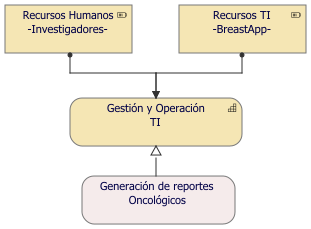
\includegraphics[width=0.77\linewidth]{ARQUITECTURA/imgs/CapaEstrategica/4_PvMapaRecurso}
	\caption{Punto de Vista de Mapa de Recurso}
	\label{PvMapaRecurso}
\end{figure}

\begin{enumerate}[label=\textbf{\arabic*})]
	

\item  \textbf{Gestión y Operación TI:} Hace referencia a la \textit{capacidad} con respecto a la gestión y operación de Tecnologías de  la Informacion del Área de Investigación de Análisis de datos para realizar el curso de acción de \textit{Implementación de tecnologías basadas en  inteligencia artificial y análisis de datos para 	mejorar  el diagnóstico de cáncer de mama}. Esta asignado a los siguientes recursos:
	
	\begin{itemize}
		\item  \textbf{\textit{Recursos Humanos:}} Este recurso hace referencia a los coordinadores, lideres técnicos,Especialistas en Oncología, científicos de datos  y desarrolladores del Área de Investigación de Análisis de datos los cuales poseen habilidades en la gestión y operación de las Tecnologías de la Informacion.
		\item  \textbf{\textit{Recursos TI:}} Este recurso hace referencia a las herramientas basadas en las Tecnologías de la Informacion que influyen en la realización de diagnósticos oncológicos. En este caso la principal herramienta para la generación de diagnósticos de cáncer de mama es la aplicación web \textit{BreastApp}.
	\end{itemize}

\item  \textbf{Generación de reportes oncológicos:} Es el paquete de trabajo principal del instituto de Cancerología basado en la estrategia planteada y los recursos disponibles identificados. La meta es construir una  aplicación web que genere  informes tipo reporte con base a los resultados arrojados por  diferentes modelos de Machine Learning, en donde se de un resultado definitivo acerca del  padecimiento de Cáncer de mama.Este diagnostico se realiza con el propósito de dar soporte a los investigadores de la Subdirección de Investigaciones, otras Subdirecciones y demás unidades funcionales del Instituto  de Cancerología.
	
\end{enumerate}














	\chapter{Capa de Negocio}
\section{Introducción}

Esta capa consiste en entender los conceptos que definen la estructura estática de la organización en términos de las entidades que componen la organización y las interacciones presentadas entre estas. Entidades como actores de negocio, roles de negocio, funciones de negocio, etc, que se comportan por medio de un diseño orientado al servicio, es decir, las funciones o procesos de negocio interno y externo de la organización como las responsabilidades \cite{BolanosCastro2019}.

Por otra parte, es importante resaltar que, dentro de la arquitectura de negocio se tiene que la relación entre entidades como se menciona anteriormente, de forma externa e interna, determina un proceso de comunicación entre estas, contando con interfaces que permiten el acceso a diferentes servicios mediante colaboraciones dadas por las entidades organizacionales \cite{BolanosCastro2019}.

A continuación se presentan cada uno de los puntos de vista de la capa de negocio  a partir del soporte realizado por el Área de Investigación de Análisis de datos a los investigadores de la Subdirección de Investigaciones, otras Subdirecciones y demás unidades funcionales del Instituto  de Cancerología.

%-------------Punto de Vista de la Organización----------%
\newpage
\section{Punto de Vista de la Organización}
El Punto de Vista de Organización se centra en la organización interna de una empresa, un departamento, una red de empresas o de otra entidad organizativa. Se utiliza para identificar las competencias, la autoridad y las responsabilidades en una organización\cite{BolanosCastro2019}.

En la Figura \ref{PvOrganizacion}, se plantea el Caso para el Punto de Vista de Organización con cada uno de los elementos que interactúan entre sí. 

\begin{figure}[h!]
	\centering
	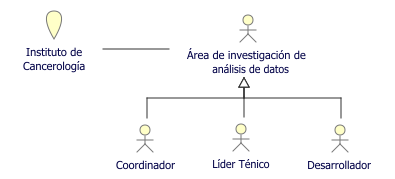
\includegraphics[width=1\linewidth]{ARQUITECTURA/imgs/CapaNegocio/1_PvOrganizacion}
	\caption{Punto de Vista de la Organización}
	\label{PvOrganizacion}
\end{figure}

\begin{enumerate}[label=\textbf{\arabic*})]
\item  \textbf{\textbf{Instituto  de Cancerología}:} Este elemento hace referencia a la localización geográfica donde se encuentra ubicada  la organización. El instituto de  Cancerología cuenta con siete grupos de investigación que desarrollan diversas actividades según su campo de acción: investigación clínica, investigación epidemológica, biología del cáncer e investigación en el área de la salud pública.Esta localización está asociada al actor \textit{Área de investigación de análisis de datos}.


\item \textbf{Área de Investigación de análisis de datos:} Corresponde a una de las dependencias del área de investigación la cual  tiene por objetivo dar soporte a los investigadores de la Subdirección de Investigaciones, otras Subdirecciones y demás unidades funcionales del Instituto  de Cancerología, haciendo uso de métodos computacionales para el manejo y análisis de datos Oncológicos. Este actor tiene como \textit{especialización} tres actores los cuales se muestran a continuación:
\newpage
\begin{itemize}
    \item  \textbf{\textit{Coordinador:}}
	Es la persona encargada de regular, gestionar, dirigir y supervisar el Área de Investigación de análisis de datos de Oncología para que el soporte realizado a los investigadores de la Subdirección de Investigaciones, otras Subdirecciones y demás unidades funcionales se realice correctamente.
	
	\item  \textbf{\textit{Líder Técnico:}}
	Es la persona con conocimiento técnico avanzado en los temas de análisis de datos de Oncología y es el  responsable de asignar y definir las  tareas y el tiempo necesario en el desarrollo e implementación de los recursos  según las necesidades presentadas por los investigadores y las unidades funcionales del Instituto  de Cancerología.
	\item  \textbf{\textit{Desarrollador:}}
	Es la persona encargada de cumplir con las implementaciones presentadas en el ámbito de análisis de datos de Oncología y que da  solución a cada uno de los requerimientos y necesidades presentadas por los  investigadores y las unidades funcionales del Instituto  de Cancerología.
	
\end{itemize}

\end{enumerate}

%-------------Punto de Vista de Cooperación de Actor---------%
\newpage
\section{Punto de Vista de Cooperación de Actor}
El Punto de Vista de Cooperación de Actor se centra en las relaciones de los actores entre sí y su entorno. Se utiliza para determinar las dependencias externas y colaboraciones, y muestra la cadena de valor o la red en la que actúa el actor\cite{BolanosCastro2019}.

En la Figura \ref{PvCooperacionActor}, se plantea el Caso para el Punto de Vista de cooperación de Actor donde se describen los elementos que interactúan este punto de vista.

\begin{figure}[h!]
	\centering
	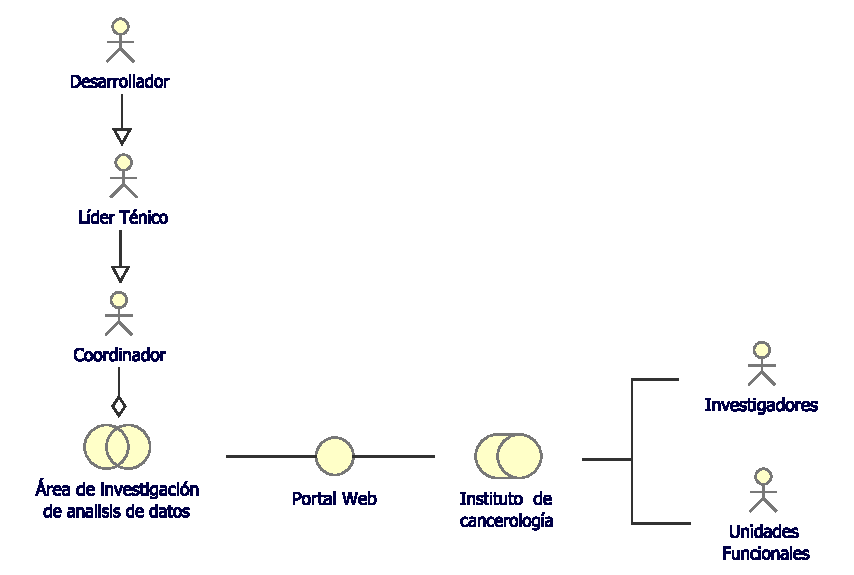
\includegraphics[width=1\linewidth]{ARQUITECTURA/imgs/CapaNegocio/2_PvCooperacionActor}
	\caption{Punto de Vista de Cooperación de Actor}
	\label{PvCooperacionActor}
\end{figure}

\begin{enumerate}[label=\textbf{\arabic*})]
\item  \textbf{Portal Web :} Es el medio de comunicación entre el Área de Investigación de análisis de datos  y los investigadores de la Subdirección de Investigaciones, otras Subdirecciones y demás unidades funcionales del Instituto  de Cancerología. Esta interfaz tiene una asociación con el rol del  \textit{Área de Investigación de análisis de datos}  y es usada por el rol \textit{Instituto  de Cancerología}.

\newpage
\item  \textbf{Instituto  de Cancerología:} A el rol  instituto de  de cancerología están asociados el actor \textit{Investigador } y el actor \textit{Unidades funcionales }. Estos roles se describen a continuación: 
\begin{itemize}
\item  \textbf{\textit{Investigadores :}}  Este rol está conformado por todos los grupos de investigación en cáncer del país registrados ante Colciencias y adicionalmente, con representantes de diferentes tipos de usuarios del conocimiento generado por la investigación como son las sociedades médicas, los prestadores de servicios oncológicos, los aseguradores, las autoridades sanitarias y los pacientes entre otros. 

\item  \textbf{\textit{Unidades Funcionales :}}  Este rol está conformado por las unidades clínicas ubicadas al interior del Instituto  de Cancerología cuya función es evaluar la situación de salud del paciente con diagnóstico presuntivo de cáncer. 
\end{itemize}
\end{enumerate}

%-------------Punto de Vista de Cooperación de Actor------------------------%
\newpage
\section{Punto de Vista de la Función de Negocio}
El Punto de Vista de la Función de Negocio muestra las principales funciones de negocio de una organización y sus relaciones en términos de los flujos de información, valor o bienes entre
ellos.

Adicionalmente, proporciona una visión de alto nivel de las operaciones generales de la empresa y puede utilizarse para identificar las competencias necesarias o estructurar una organización de acuerdo con sus principales actividades
\cite{BolanosCastro2019}.

En la Figura \ref{PvFuncion}, se plantea el Caso para el Punto de Vista de Función de Negocio donde se describen los elementos que interactúan en este punto de vista.

\begin{figure}[h!]
	\centering
	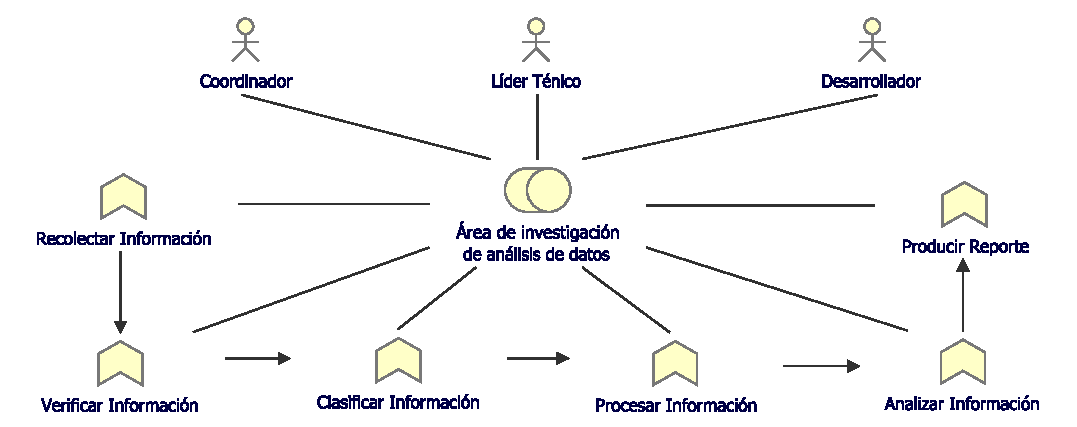
\includegraphics[width=1\linewidth]{ARQUITECTURA/imgs/CapaNegocio/3_PvFuncion}
	\caption{Punto de Vista de la Función del negocio}
	\label{PvFuncion}
\end{figure}

\begin{enumerate}[label=\textbf{\arabic*})]
\item  \textbf{Área de Investigación de análisis de datos:} Este rol corresponde  a una de las dependencias del área de investigación la cual  tiene por objetivo dar soporte a los investigadores de la Subdirección de Investigaciones, otras Subdirecciones y demás unidades funcionales del Instituto  de Cancerología. Este rol está asociado a los actores coordinador, líder técnico y desarrollador y a seis diferentes funciones las cuales se muestran a continuación:
\newpage
\begin{itemize}
\item  \textbf{\textit{Recolectar Datos:}} Esta función se encarga de recopilar y medir la información de los Data Set que contienen variables oncológicas específicas que requieren ser analizadas.

\item  \textbf{\textit{Verificar Datos:}}  Esta función se basa en la identificación  y corrección o eliminación de registros de datos erróneos encontrados en los Data Set oncológicos. Este proceso permite encontrar datos incompletos, incorrectos, inexactos, no pertinentes, etc. y luego substituir, modificar o eliminar para realizar posteriormente la clasificación de los mismos.

\item  \textbf{\textit{Clasificar Datos:}} Esta función se basa en la distribución por medio de algoritmos de Machine Learning de los Data Set que contienen variables oncológicas específicas que al ser comparados con trazas características de casos de cáncer avanzados permiten agruparlos en diferentes categorías según el porcentaje de padecimiento del mismo.

\item  \textbf{\textit{Procesar Datos:}} Esta función se basa en la manipulación de los Data Set oncológicos  para generar información por medio de gráficos y estadísticas haciendo uso de los modelos de Machine Learning.

\item  \textbf{\textit{Analizar Datos:}} Esta función se encarga de examinar los Data Set que dieron como resultado de las funciones anteriores y los gráficos obtenidos con el propósito de sacar conclusiones diagnosticas sobre el posible padecimiento de cáncer.

\item  \textbf{\textit{Generar Reportes:}} Esta función se encarga de crear en un módulo informativo los datos relevantes obtenidos de los Data Set oncológicos solicitados para ser analizados por medio de tablas, estadísticas y gráficos que dan el resumen de los resultados, conclusiones y diagnósticos sobre el posible padecimiento de cáncer en el individuo.
\end{itemize}
\end{enumerate}

%-------------Punto de Vista de Proceso de Negocio------------------------%
\newpage
\section{Punto de Vista de Proceso de Negocio}
El Punto de Vista de Proceso de Negocio se utiliza para mostrar la estructura y composición de alto nivel de uno o más procesos empresariales\cite{BolanosCastro2019}.

Junto a los procesos mismos, este punto de vista contiene otros conceptos directamente relacionados, tales como: los servicios que un proceso de negocio ofrece de manera global, mostrando como un proceso contribuye a la realización de los productos de la empresa; la asignación de los procesos de negocio a las funciones, lo que da una idea de las responsabilidades de los actores asociados; la información utilizada por el proceso de negocio. Cada uno de estos puede ser considerado como una sub-vista de la vista del proceso empresarial\cite{BolanosCastro2019}.

En la Figura \ref{PvProceso}, se plantea el Caso para el Punto de Vista de Proceso de Negocio aplicado al Área de Investigación de análisis de datos. A continuación, se describen los elementos que interactúan en este punto de vista.

\begin{figure}[h!]
	\centering
	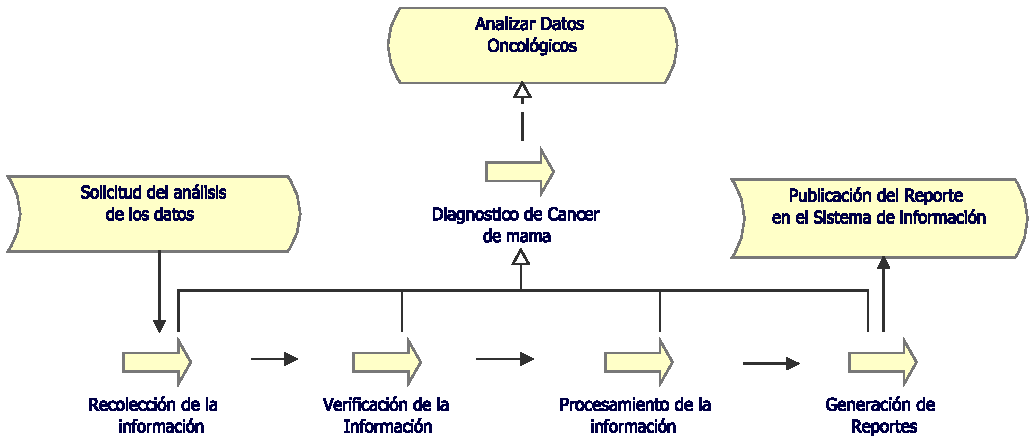
\includegraphics[width=1\linewidth]{ARQUITECTURA/imgs/CapaNegocio/4_PvProceso}
	\caption{Punto de Vista del proceso del negocio}
	\label{PvProceso}
\end{figure}

\begin{enumerate}[label=\textbf{\arabic*})]
	\item  \textbf{Analizar Datos Oncológicos:} Este servicio realiza el análisis de los datos entregados por  los investigadores de la Subdirección de Investigaciones, otras Subdirecciones y demás unidades funcionales del Instituto  de Cancerología para generar diagnósticos oncológicos. Es brindando por el proceso de  \textit{Análisis de Datos}.
	\newpage
	\item  \textbf{Diagnostico de Cáncer de mama:} El proceso de Diágnostico de Cáncer de mama es fundamental debido que cumple con el objetivo principal de facilitar el análisis de datos oncológicos a las diferentes áreas y unidades funcionales de la organización. Además, este proceso está conformado de otros procesos en secuencia que dan solución al servicio final.

	\item  \textbf{Solicitud de análisis de datos:} Este evento es el que origina los sub-procesos para lograr el objetivo del servicio principal. Este corresponde a la acción en donde  los investigadores de la Subdirección de Investigaciones, otras Subdirecciones y demás unidades funcionales del Instituto  de Cancerología desean que se analicen diferentes Data Set oncológicos para obtener un reporte. Está relacionado  directamente con el sub-proceso de \textit{Recolección de información}  que es el primer proceso para analizar los datos solicitados.
	
	\item  \textbf{Recolección de información:} Este sub-proceso se encarga de recopilar y organizar toda la información que contiene datos oncológicos de cada paciente que son necesarios para su posterior verificación. Es el primer subproceso llevado a cabo para el objetivo de análisis de datos oncológicos que a su vez, desencadena un nuevo subproceso mediante una relación causal.
	
	\item  \textbf{Verificación de la información:} Este sub-proceso se encarga de identificar si las variables oncológicas solicitadas están completas. Además, si la información entregada esta completa pero algunos de los datos se encuentran erróneos o defectuosos se sustituyen para realizar posteriormente la clasificación de los mismos. Este sub-proceso desencadena un nuevo subproceso mediante una relación causal.
	
	\item  \textbf{Procesamiento de la información:} Este sub-proceso se encarga de usar los datos oncológicos  verificados para generar información relevante por medio de gráficos y estadísticas. Este sub-proceso desencadena un nuevo subproceso mediante una relación causal.
	
	\item  \textbf{Generación  de Reportes:} Este sub-proceso se encarga de organizar en un módulo la información de los resultados obtenidos de los Data Set oncológicos solicitados para ser analizados por medio de tablas, estadísticas y gráficos. Este sub-proceso desencadena un nuevo subproceso mediante una relación causal.
	\newpage
	\item  \textbf{Publicación del Reporte en el portal web :} Este evento es el que finaliza el flujo conformado por los sub-procesos anteriores y representa la acción de difundir la información oncológica analizada y  los resultados diagnósticos obtenidos en el Portal web  de cada uno de los datos solicitados para análisis. Este evento es accionado por el sub-proceso \textit{Generación  de Reportes}.
\end{enumerate}

%-------------Punto de Vista de Cooperación de Proceso de Negocio}o------------------------%
\newpage
\section{Punto de Vista de Cooperación de Proceso de Negocio}
El Punto de Vista de Cooperación de Proceso de Negocio se utiliza para mostrar las relaciones de uno o más procesos de negocio entre si y/o con su entorno\cite{BolanosCastro2019}.

Puede utilizarse tanto para crear un diseño de alto nivel de procesos empresariales dentro de su contexto, como para proporcionar un gestor operativo responsable de uno o más de dichos procesos con información sobre sus dependencias \cite{BolanosCastro2019}.

En la Figura \ref{PvCooperacionProces}, se plantea el Caso para el Punto de Vista de Cooperación de Proceso de Negocio aplicado al Área de Investigación de análisis de datos. A continuación, se describen los elementos que interactúan en el punto de vista.

\begin{figure}[h!]
	\centering
	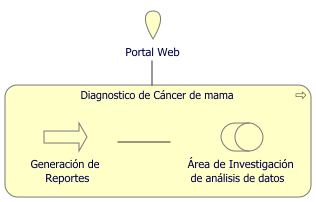
\includegraphics[width=0.75\linewidth]{ARQUITECTURA/imgs/CapaNegocio/5_PvCooperacionProceso}
	\caption{Punto de Vista de Cooperación de Proceso de Negocio}
	\label{PvCooperacionProces}
\end{figure}

\begin{enumerate}[label=\textbf{\arabic*})]
\item  \textbf{Portal Web :} Es el medio de comunicación entre el Área de Investigación de análisis de datos  y los investigadores de la Subdirección de Investigaciones, otras Subdirecciones y demás unidades funcionales del Instituto  de cancerología. Está relacionado directamente con el servicio de \textit{Diagnostico de Cáncer de mama}. 

\item  \textbf{Diagnóstico de Cáncer de mama:} Este servicio cumple el objetivo dar soporte a los investigadores de la Subdirección de Investigaciones, otras Subdirecciones y demás unidades funcionales del Instituto  de Cancerología con respecto al análisis de datos oncológicos.  Es brindado por el proceso de \textit{Análisis de Datos}.
\newpage
\item  \textbf{Generación  de Reportes:} Este sub-proceso hace referencia a la organización de la información de los resultados obtenidos de los Data Set oncológicos solicitados para ser analizados por medio de tablas, estadísticas y gráficos.

\item \textbf{Área de Investigación de análisis de datos:} Corresponde área de investigación la cual da soporte a los investigadores de la Subdirección de Investigaciones, otras Subdirecciones y demás unidades funcionales del Instituto  de Cancerología por medio reportes generados con base a los datos solicitados.

\end{enumerate}

%-------------Punto de Vista de Producto-----------------------------%
\newpage
\section{Punto de Vista de Producto}
El Punto de Vista de Producto representa el valor que estos productos ofrecen a los clientes u otras partes externas involucradas\cite{BolanosCastro2019}.

Adicionalmente, muestra la composición de uno o más productos en términos de los servicios constitutivos-comerciales o de aplicación, y los contratos asociados u otros acuerdos. También se puede utilizar para mostrar las interfaces a través de las cuales se ofrece este producto, y los eventos asociados al mismo\cite{BolanosCastro2019}.

En la Figura \ref{PvProducto}, se plantea el Caso para el Punto de Vista de Producto.A continuación, se describen los elementos que interactúan en el punto de vista.

\begin{figure}[h!]
	\centering
	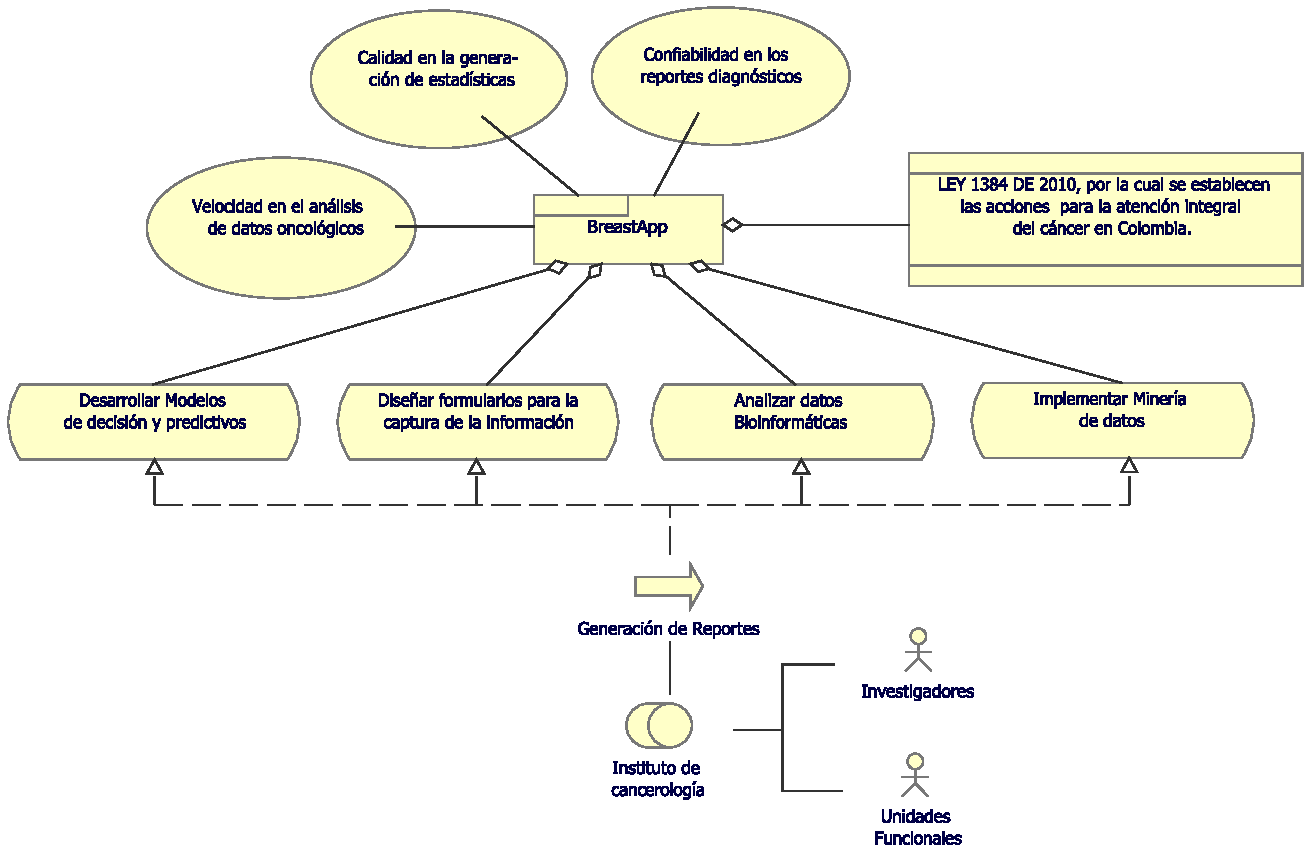
\includegraphics[width=1\linewidth]{ARQUITECTURA/imgs/CapaNegocio/6_PvProducto}
	\caption{Punto de Vista de Producto}
	\label{PvProducto}
\end{figure}

\begin{enumerate}[label=\textbf{\arabic*})]
	
	\item  \textbf{BreastApp:} Este producto corresponde a la generación de reportes diagnósticos según el análisis de datos oncológicos elaborados por los investigadores de la Subdirección de Investigaciones, otras Subdirecciones y demás unidades funcionales del Instituto  de Cancerología. Está compuesto de los siguientes servicios:
	
\begin{itemize}
	\item  \textbf{\textit{Desarrollar Modelos de Decisión y predictivos:}} Este servicio corresponde al uso de modelos de Machine Learning para  para diagnosticar  el padecimiento de cáncer .Este servicio sirve como herramienta para realizar diversas investigaciones y poder  disminuir su tasa de mortandad en Colombia.
	
	\item  \textbf{\textit{Diseñar formularios para la captura de la información:}} Este servicio corresponde a la creación de formularios web de ámbito científico con énfasis en el diagnóstico del cáncer para que los diferentes investigadores y áreas funcionales de la organización proporcionen la información relacionada con los datos de cada individuo.
	
	\item  \textbf{\textit{Analizar Datos Bioinformáticos:}} Este servicio corresponde a los métodos y modelos basados en diferentes sistemas de cómputo numéricos con base a variables del ámbito de la biología para realizar simulaciones que permitan observar el comportamiento de los mismos en diferentes ambientes y determinar una posible solución al problema del padecimiento de cáncer.
	
	\item  \textbf{\textit{Implementar Minería de Datos:}} Este servicio corresponde a la búsqueda de  correlaciones o patrones entre los millones de datos obtenidos de todos los pacientes con cáncer para proporcionar información diagnostica cada vez más específica y exacta de los datos solicitados por los investigadores y las unidades funcionales de la organización.
\end{itemize}
	Ademas, cuenta son los siguientes valores:
\begin{itemize}
		\item  \textbf{\textit{Velocidad en el análisis de datos oncológicos:}} El objetivo principal es realizar de manera eficaz el análisis los datos oncológicos en cuestión para dar una diagnostico  en el menor tiempo posible.
		
		\item  \textbf{\textit{Calidad en la generación de estadísticas:}} El objetivo principal es analizar los datos de una manera profesional   para satisfacer necesidades explícitas de los investigadores y las unidades funcionales de la organización. 
		
		\item  \textbf{\textit{Confiabilidad en los reportes diagnósticos:}} El objetivo principal es generar los reportes oncológicos analizados  con una precisión superior para que la información generada por tablas y gráficos generen un diagnóstico exacto que ayude en las diferentes actividades de los investigadores y las unidades funcionales de la organización.
		
\end{itemize}

	\item  \textbf{Ley 1384 de 2010:} Esta resolución establece las acciones para el control integral del cáncer en la población colombiana, de manera que se reduzca la mortalidad y la morbilidad por cáncer adulto, así como mejorar la calidad de vida de los pacientes oncológicos, a través de la garantía por parte del Estado y de los actores que intervienen en el Sistema General de Seguridad Social en Salud vigente, de la prestación de todos los servicios que se requieran para su prevención, detección temprana, tratamiento integral, rehabilitación y cuidado paliativo.
	
	\item  \textbf{Generación de Reportes:} Implica la organización de la información de los resultados obtenidos en los diagnósticos oncológicos solicitados para ser visualizados por medio de tablas, estadísticas y gráficos. Se asocia con el rol de \textit{Instituto  de cancerología}. A su vez, realiza los servicios descritos anteriormente.
	
	
	\item  \textbf{Instituto  de Cancerología:} Este elemento hace referencia el rol  Instituto de  de cancerología el cual cuenta con siete grupos de investigación que desarrollan diversas actividades según su campo de acción: investigación clínica, investigación epidemiológica, biología del cáncer e investigación en el área de la salud pública. Este rol usa el proceso \textit{Generación de Reporte} y se asigna a los dos actores a continuación:
	
	\begin{itemize}
		\item  \textbf{\textit{Investigadores :}}  Este rol está conformado por todos los grupos de investigación en cáncer del país registrados ante Colciencias y adicionalmente, con representantes de diferentes tipos de usuarios del conocimiento generado por la investigación como son las sociedades médicas, los prestadores de servicios oncológicos, los aseguradores, las autoridades sanitarias y los pacientes entre otros. 
		
		\item  \textbf{\textit{Unidades Funcionales :}}  Este rol está conformado por las unidades clínicas ubicadas al interior del Instituto  de Cancerología cuya función es evaluar la situación de salud del paciente con diagnóstico presuntivo de cáncer. 
	\end{itemize}
	
\end{enumerate}
	\chapter{Capa de Aplicación}
\section{Introducción}
Esta capa retoma la mayoría de conceptos  utilizados en la capa de negocio con la distinción de los diferentes usos e interacciones que se presentan. Para una adecuada apropiación de los conceptos de esta capa, se implementa el uso de cuatro diferentes puntos  de vista: comportamiento, cooperación, estructura y uso de la aplicación \cite{BolanosCastro2019}.

Entidades como componentes y objeto de datos que se comportan por medio de una relación explicita en el modelo, es decir, el comportamiento a nivel interno y externo de la organización; el comportamiento externo dado en términos de los servicios de aplicación mientras que el comportamiento interno en funciones de aplicación que realizan estos servicios \cite{BolanosCastro2019}.

Dentro de la arquitectura de aplicación un aspecto fundamental corresponde a las interrelaciones de componentes, que determinan la comunicación entre estos, contando con el concepto de colaboración. Además, el concepto de interfaz que se define como el canal lógico mediante el cual se accede a un servicio de componente, detalla características de comportamiento tales como el conjunto de operaciones y eventos que expone el componente \cite{BolanosCastro2019}.

También, se puede distinguir los servicios de aplicaciones internas (comunicación de aplicación a aplicación) y servicios de aplicaciones externas (comunicación de aplicación a negocio), ambos servicios presentados por la interfaz de aplicación \cite{BolanosCastro2019}.

A continuación se presentan cada uno de los puntos de vista de la capa de aplicación a partir del soporte realizado por el Área de Investigación de Análisis de datos a los investigadores de la Subdirección de Investigaciones, otras Subdirecciones y demás unidades funcionales del Instituto de Cancerología.

%-------------Punto de Vista Comportamiento Aplicacion----------%
\newpage
\section{Punto de Vista del Comportamiento de la Aplicación}
El Punto de Vista de comportamiento de la aplicación describe el comportamiento interno de una aplicación, es útil para diseñar el comportamiento principal de las aplicaciones o para identificar la superposición funcional entre las mismas.\cite{BolanosCastro2019}.

En la Figura \ref{PvComportamientoApp} se plantea el Caso para el Punto de Vista del comportamiento de la aplicación con cada uno de los elementos que interactúan entre sí. 

\begin{figure}[h!]
	\centering
	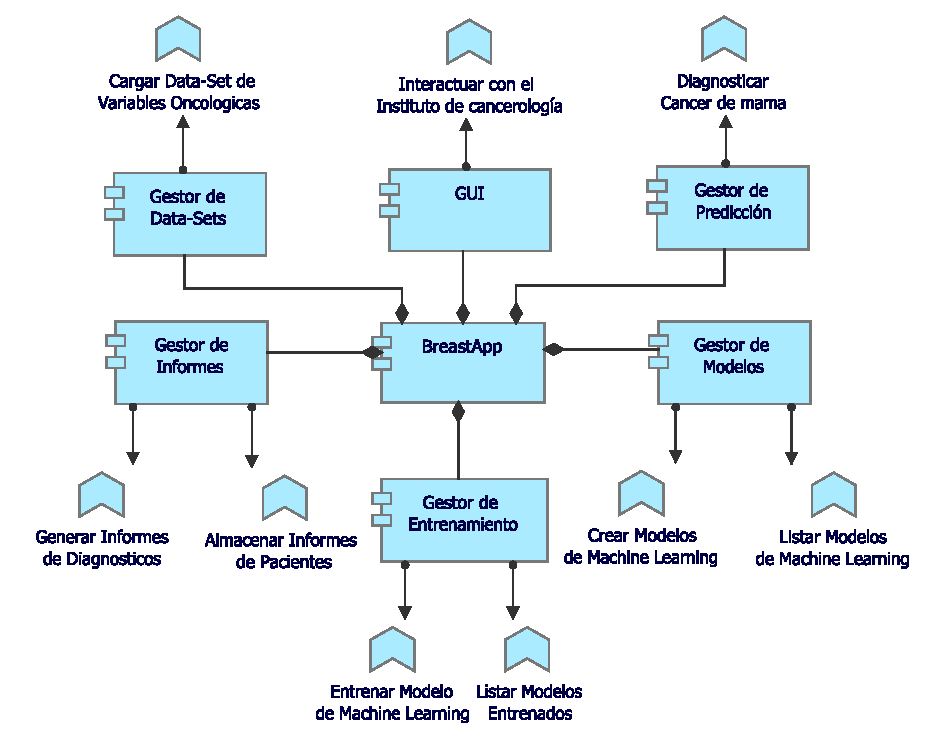
\includegraphics[width=1\linewidth]{ARQUITECTURA/imgs/CapaAplicacion/1_PvComportamientoApp}
	\caption{Punto de Vista del Comportamiento de la  Aplicación}
	\label{PvComportamientoApp}
\end{figure}

\begin{enumerate}[label=\textbf{\arabic*})]
	
\item  \textbf{BreastApp:} El componente de BreastApp es el framework  de la aplicación. En este componente se agregan los componentes correspondientes para el diagnóstico de cáncer de mama y se realiza la carga de modelos, carga de Data-Sets, entrenamiento de modelos  y generación de informes  sobre el cáncer de mama.

\item  \textbf{GUI:} Este componente esta agregado al componente principal de BreastApp. Este componente hace referencia a la interfaz gráfica de usuario por la cual los investigadores y unidades funcionales del Instituto  de Cancerología acceden a la aplicación, para llevar el análisis según diagnostico de cáncer de mama generado por la aplicación.Este componente cumple con la siguientes funciones:

	
\begin{itemize}
	\item  \textbf{\textit{Interactuar con el Instituto de Cancerologia:}} Hace referencia a las acciones y herramientas que contiene el Front-End de la aplicacion BreastApp las cuales pueden ser usadas po los investigadores de la Subdirección de Investigaciones, otras Subdirecciones y demás unidades funcionales del Instituto de Cancerología 
\end{itemize}
	
\item  \textbf{Gestor de Data-Sets:} Este componente esta agregado al componente principal de BreastApp. En este componente se maneja el proceso de carga  y gestión de Data-Sets para ser almacenados en el sistema.Este componente cumple con la siguientes funciones:
	
	\begin{itemize}
		\item  \textbf{\textit{Cargar Data-Set de Variables Oncológicas :}} Hace referencia a la carga del Data-Set para entrenamiento de los Modelos en Machine Learning y el Data-Set que contiene las variables Oncológicas de los pacientes a los cuales se les quiere detectar el padecimiento de cáncer de mama.
	\end{itemize}

\item  \textbf{Gestor de Entrenamiento:} Este componente esta agregado al componente principal de BreastApp. En este componente se maneja el proceso de entrenamientos de los modelos de Machine Learning haciendo uso de los Data-Sets  que estén almacenados en el sistema.Este componente cumple con la siguientes funciones:

	\begin{itemize}
		\item  \textbf{\textit{Entrenar Modelos de Machine Learning :}} Esta función realiza la mejora incremental para la predicción con Base en el Data-Set que contiene variables con resultados ya definidos de pacientes a los que ya se les detecto si el cáncer de mama era maligno o Benigno.
		
		\item  \textbf{\textit{Listar Modelo Entrenados:}} Esta función realiza una lista de los modelos a  los cuales ya se les realizo una mejora incremental de predicción para no repetir el proceso de entrenamiento cada vez que se requiere un diagnostico de cáncer de mama de diversos pacientes.
	\end{itemize}

\newpage
\item  \textbf{Gestor de Predicción:} Este componente esta agregado al componente principal de BreastApp. En este componente se maneja el proceso de diagnosticar el padecimiento de cáncer de mama. Este componente cumple con la siguiente función:
	\begin{itemize}
		\item  \textbf{\textit{Diagnosticar Cáncer de mama:}} Esta función realiza el diagnostico de cáncer de mama con base al entrenamiento anteriormente realizado , las variables de nuevos pacientes a los que se requiere realizar el análisis ontológico y las diversas técnicas de predicción y decisión de Machine Learning. 
	\end{itemize}

\item  \textbf{Gestor de Informes:} Este componente esta agregado al componente principal de BreastApp. En este componente se maneja el proceso generar informes con detalles del diagnóstico.Este componente cumple con la siguientes funciones:

\begin{itemize}
	\item  \textbf{\textit{Generar Informes de Diagnósticos:}} Esta función genera los informes tipo reporte con base a los resultados arrojados por los diferentes Modelos en Machine Learning, en donde se da un resultado definitivo acerca del  padecimiento de Cáncer de mama.
	
	\item  \textbf{\textit{Almacenar Informes de Pacientes:}} Esta función almacena los diferentes informes determinados a los pacientes a los que se quiere determinar el padecimiento de cáncer de mama.
\end{itemize}

\item  \textbf{Gestor de Modelos:} Este componente esta agregado al componente principal de BreastApp. En este componente se maneja el proceso implementación de  modelos de Machine Learning.Este componente cumple con la siguientes funciones:

\begin{itemize}
	\item  \textbf{\textit{Crear Modelos de Machine Learning:}} Esta función asocia los Data-Sets a los modelos de Machine Learning con los que realiza el respectivo diagnostico.
	
	\item  \textbf{\textit{Listar Modelos de Machine Learning:}} Esta función permite obtener los modelos de Machine Learning que utiliza el aplicativo de BreastApp.
\end{itemize}	
		
\end{enumerate}

%-------------Punto de Vista de Cooperación de Aplicación----------%
\newpage
\section{Punto de Vista de Cooperación de Aplicación}
El Punto de Vista de cooperación de la aplicación describe las relaciones entre los componentes de las aplicaciones en términos de los flujos de información entre ellos o en términos de los servicios que ofrecen y utilizan.\cite{BolanosCastro2019}.

En la Figura \ref{PvCooperacionApp} se plantea el Caso para el Punto de Vista de cooperación de la aplicación con cada uno de los elementos que interactúan entre sí. 

\begin{figure}[h!]
	\centering
	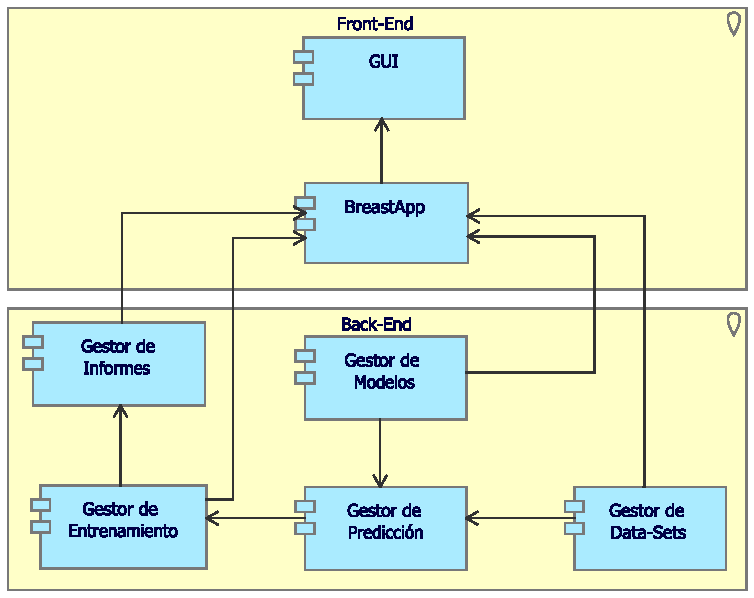
\includegraphics[width=1\linewidth]{ARQUITECTURA/imgs/CapaAplicacion/2_PvCooperacionApp}
	\caption{Punto de Vista de Cooperación de la Aplicación}
	\label{PvCooperacionApp}
\end{figure}

\begin{enumerate}[label=\textbf{\arabic*})]

\item  \textbf{BreastApp:} El componente de BreastApp es el framework  de la aplicación. En este se componente agregan los componentes correspondientes para el diagnóstico de cáncer de mama y se realiza la carga de modelos, carga de Data-Sets, entrenamiento de modelos  y generación de informes  sobre el cáncer de mama.
\item  \textbf{GUI:} Este componente esta agregado al componente principal de BreastApp. Este componente hace referencia a la interfaz gráfica de usuario por la cual los investigadores y unidades funcionales del Instituto  de Cancerología acceden a la aplicación, para llevar el análisis según el diagnostico de cáncer de mama generado por la aplicación.

\item  \textbf{Gestor de Modelos:} Este componente es usado por el componente principal de BreastApp y el componente Gestor de entrenamiento. En este componente se maneja el proceso de crear modelos.

\item  \textbf{Gestor de Predicción:} Este componente es usado por el componente de Gestor de Data-Sets y el componente Gestor de Modelos.En este componente se maneja el proceso de diagnosticar padecimiento de cáncer de mama.

\item  \textbf{Gestor de Data-Sets:} Este componente es usado por el componente principal de BreastApp y el componente Gestor de Predicción . En este componente se maneja el proceso de carga  y gestión de Data-Sets para ser almacenados en el sistema.

\item  \textbf{Gestor de Entrenamiento:} Este componente es usado por el componente principal de BreastApp y  el componente de Gestor de Predicción. En este componente se maneja el proceso de entrenamientos de los modelos de Machine Learning haciendo uso de los Data-Sets  que estén almacenados en el sistema.

\item  \textbf{Gestor de Informes:} Este componente es usado por el componente principal de BreastApp. En este componente se maneja el proceso Generar informes con detalles del diagnóstico.

\end{enumerate}


%-------------Punto de Vista de Estructura de Aplicación----------%
\newpage
\section{Punto de Vista de la Estructura de la Aplicación}
El Punto de Vista de estructura de la aplicación describe la estructura principal de aplicaciones o componentes y los datos asociados.\cite{BolanosCastro2019}.

En la Figura \ref{PvEstructuraApp} se plantea el Caso para el Punto de Vista de la estructura de la aplicación con cada uno de los elementos que interactúan entre sí. 

\begin{figure}[h!]
	\centering
	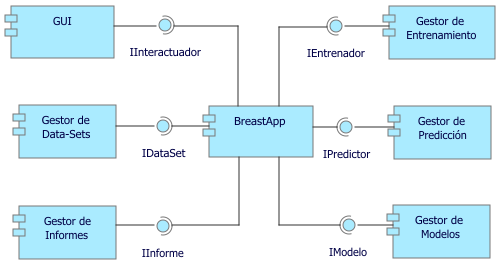
\includegraphics[width=1\linewidth]{ARQUITECTURA/imgs/CapaAplicacion/3_PvEstructuraApp}
	\caption{Punto de Vista de la Estructura  de la Aplicación}
	\label{PvEstructuraApp}
\end{figure}

\begin{enumerate}[label=\textbf{\arabic*})]
	
	\item  \textbf{BreastApp:} El componente de BreastApp es el framework  de la aplicación. En este se componente agregan los componentes correspondientes para el diagnóstico de cáncer de mama y se realiza la carga de modelos, carga de Data-Sets, entrenamiento de modelos  y generación de informes  sobre el cáncer de mama.
	\item  \textbf{GUI:} Este componente esta agregado al componente principal de BreastApp. Este componente hace referencia a la interfaz gráfica de usuario por la cual los investigadores y unidades funcionales del Instituto  de Cancerología acceden a la aplicación, para llevar el análisis según diagnostico de cáncer de mama generado por la aplicación, a través de la interfaz \textit{IInteractuador}.
	
	\item  \textbf{Gestor de Data-Sets:}Este componente ofrece un servicio a través de la interfaz \textit{IDataSet} al componente principal de BreastApp. En este componente se maneja el proceso de carga  y gestión de Data-Sets para ser almacenados en el sistema.
		
	\item  \textbf{Gestor de Informes:}Este componente ofrece un servicio a través de la interfaz \textit{IInforme} al componente principal de BreastApp. Este componente es usado por el componente principal de BreastApp. En este componente se maneja el proceso Generar informes con detalles del diagnóstico de cada paciente.
	
		
	\item  \textbf{Gestor de Entrenamiento:}Este componente ofrece un servicio a través de la interfaz \textit{IEntrenador} al componente principal de BreastApp. En este componente se maneja el proceso de entrenamientos de los modelos de Machine Learning haciendo uso de los Data-Sets  que estén almacenados en el sistema.
	
	\item  \textbf{Gestor de Predicción:}Este componente ofrece un servicio a través de la interfaz \textit{IPredictor} al componente principal de BreastApp. En este componente se maneja el proceso de diagnosticar padecimiento de cáncer de mama.
	
	\item  \textbf{Gestor de Modelos:} Este componente ofrece un servicio a través de la interfaz \textit{IModelo} al componente principal de BreastApp.En este componente se maneja el proceso de crear modelos.
\end{enumerate}

%-------------Punto de Vista de Uso de Aplicación----------%
\newpage
\section{Punto de Vista del Uso de la Aplicación}
El Punto de Vista del uso de la aplicación describe el diseño de una aplicación mediante la identificación de los servicios necesarios por los procesos de negocio y otras aplicaciones, o en el diseño de procesos de negocio mediante la descripción de los servicios que están disponibles \cite{BolanosCastro2019}.

En la Figura \ref{PvusoApp} se plantea el Caso para el Punto de Vista del uso de la aplicación con cada uno de los elementos que interactúan entre sí. 

\begin{figure}[h!]
	\centering
	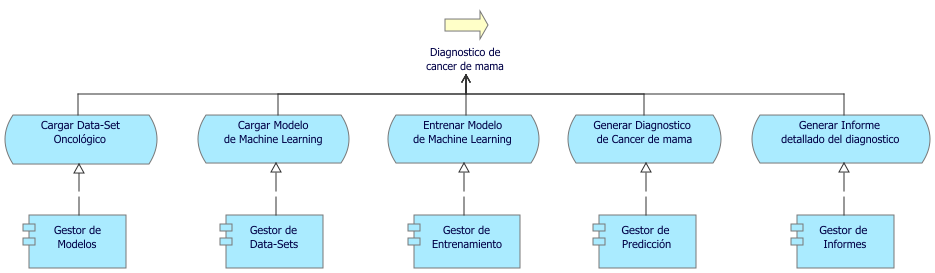
\includegraphics[width=1\linewidth]{ARQUITECTURA/imgs/CapaAplicacion/4_PvUsoApp}
	\caption{Punto de Vista del uso de la Aplicación}
	\label{PvusoApp}
\end{figure}

\begin{enumerate}[label=\textbf{\arabic*})]
	
	\item  \textbf{Diagnóstico de cáncer de mama:} Este proceso consiste en el diagnóstico de padecimiento de cáncer de mama. Es logrado mediante cinco servicios: \textit{Cargar modelo, Cargar Data-Set, Entrenar Modelo, Generar diagnóstico y Generar informe detallado del diagnóstico.} 
	
	\item  \textbf{Cargar Data-Set Oncológico:} Este servicio de la aplicación recibe los Data-Set con las variables oncológicas en formato .csv,  los valida  y los almacena en el sistema. Este servicio es realizado por el componente \textit{Gestor de Data-Sets}.
	
	\item  \textbf{Cargar Modelo de Machine Learning:} Este servicio de la aplicación es el encargado de crear modelos de Machine Learning. Este servicio es realizado por el componente \textit{Gestor de Modelos}.
	
	\item  \textbf{Generar Diagnostico de cáncer de mama:} Este servicio de aplicación recibe los datos de un paciente en particular  y realiza el diagnóstico. El servicio responde sí según los datos tiene un diagnóstico Benigno y Maligno. Este servicio es realizado por el componente \textit{Gestor de Predicción}.
	
	\item  \textbf{Generar Informe Detallado del Diagnostico:} Este servicio genera un informe detallado en formato .pdf con la información respectiva de las predicciones y gráficos de cada cada modelo.Este servicio es realizado por el componente \textit{Gestor de Informes}.
	
	

\end{enumerate}
	\chapter{Capa de Tecnología}
\section{Introducción}
Esta capa toma, en primer lugar, la utilización de conceptos como Nodo y Dispositivo para identificar las diferentes entidades físicas o recursos computacionales de la infraestructura del sistema \cite{BolanosCastro2019}.

Esta capa  busca establecer y conocer los diferentes elementos a nivel de software y hardware que interactúan en los procesos de negocio establecidos anteriormente, por lo tanto, es importante tener en cuenta los conceptos utilizados en la capa de negocio y en la capa de aplicación para así facilitar la identificación de los diferentes usos e interacciones que se presentan con esta capa. Para una adecuada apropiación de la conceptualización de esta capa, se implementa el uso de seis diferentes puntos de vista: infraestructura, uso de infraestructura, implementación y organización, estructura de información, realización de servicio y capas \cite{BolanosCastro2019}.

Por otra parte, es importante resaltar que, dentro de la infraestructura, un aspecto fundamental corresponde a las interacciones entre los diferentes elementos a nivel de software (componentes) y a nivel de hardware (dispositivos), que determinan la comunicación entre los conceptos de aplicación  y conceptos de negocio mencionados en las dos capas anteriores\cite{BolanosCastro2019}.

A continuación se presentan cada uno de los puntos de vista de la capa de tecnología  a partir del soporte realizado por el Área de Investigación de Análisis de datos a los investigadores de la Subdirección de Investigaciones, otras Subdirecciones y demás unidades funcionales del Instituto de Cancerología.

%-------------Punto de Vista de la Infraestructura----------%
\newpage
\section{Punto de Vista de la Infraestructura}
El Punto de Vista de la Infraestructura contiene los elementos de infraestructura de software y hardware que soportan la capa de aplicación, como dispositivos físicos, redes o software del sistema\cite{BolanosCastro2019}.

En la Figura \ref{PvInfraestructura}, se plantea el Caso para el Punto de Vista de la infraestructura con cada uno de los elementos que interactúan entre sí. 

\begin{figure}[h!]
	\centering
	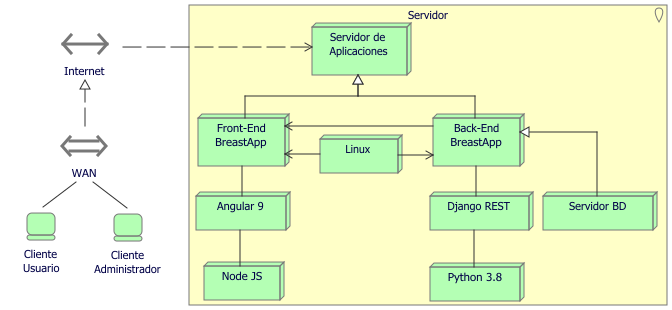
\includegraphics[width=1\linewidth]{ARQUITECTURA/imgs/CapaTecnologia/1_PvInfraestructuraTec}
	\caption{Punto de Vista de la Infraestructura}
	\label{PvInfraestructura}
\end{figure}

\begin{enumerate}[label=\textbf{\arabic*})]
	
\item  \textbf{Servidor de Aplicaciones:} Hace referencia a el nodo que se conecta directamente a la red para exponer la disponibilidad de la aplicación. Es el nodo general donde interactúan tanto componentes, como sistemas de software y demás elementos necesarios para
la aplicación.

\item \textbf{Front-End BreastApp:} Corresponde a la interfaz gráfica de usuario por la cual los investigadores y unidades funcionales del Instituto de Cancerología acceden a la aplicación, para llevar el análisis según diagnostico de cáncer de mama generado por la aplicación.

\item \textbf{Angular 9:} Hace referencia a el framework seleccionado para desarrollar  la interfaz gráfica de usuario de la aplicación BreastApp.

\item \textbf{Node JS:} Es el entorno basado en JavaScript imprescindible para poder usar el framework de Angular 9.

\item \textbf{Back-End BreastApp:} Hace referencia a el desarrollo de la lógica para la generación de la capa de servicios REST para las diferentes funcionalidades necesarias para generar el diagnostico relacionado con el cáncer de mama.

\item \textbf{Django:} Hace referencia a el framework seleccionado para desarrollar la capa de servicios REST para la aplicación BreastApp.

\item \textbf{Python 3.8:} Corresponde a el lenguaje de programación seleccionado para el desarrollo del Back-End de la aplicación BreastApp.

\item \textbf{Linux:} Este sistema de software es el sistema operativo donde se desarrolla el Back-End y Front-End de la aplicación BreastApp.

\item \textbf{Servidor BD:} Este sistema de software hace referencia a la persistencia de los datos de la aplicación BreastApp. Se realiza  automáticamente en el Back-End de la aplicación por medio del framework Django.

\item \textbf{Internet:} Hace referencia a el acceso a la aplicación  través de la red, debido a que los  investigadores y unidades funcionales del Instituto de Cancerología podrán acceder desde sus casas o lugares externos.

\item \textbf{WAN:}  Debido a  que los usuarios pueden acceder desde cualquier punto,
es necesario una red de área amplia que reúna varias redes locales y brinde la conexión a los investigadores y unidades funcionales del Instituto de Cancerología. 

\item \textbf{Cliente:} En la aplicación BreastApp, existen dos tipos de clientes:

\begin{itemize}
	\item  \textbf{\textit{Cliente Usuario:}} Hace referencia a los  investigadores y unidades funcionales del Instituto de Cancerología.
	
	\item  \textbf{\textit{Cliente Administrador:}} Hace referencia a las personas autorizadas de administrar el uso y funcionamiento de la aplicación BreastApp, así como utilizar la información del Instituto de Cancerología de manera pertinente.
\end{itemize}
\end{enumerate}

%-------------Punto de Vista de la Infraestructura----------%
\newpage
\section{Punto de Vista del Uso de la Infraestructura}
El Punto de Vista del uso de la  Infraestructura describe como las aplicaciones son compatibles con la infraestructura de software y hardware. Es muy útil para determinar los requisitos de
rendimiento y calidad de la infraestructura basados en las demandas de las diversas aplicaciones que la utilizan \cite{BolanosCastro2019}.

En la Figura \ref{PvUsoInfraestructura}, se plantea el Caso para el Punto de Vista del Uso de la infraestructura con cada uno de los elementos que interactúan entre sí. 

\begin{figure}[h!]
	\centering
	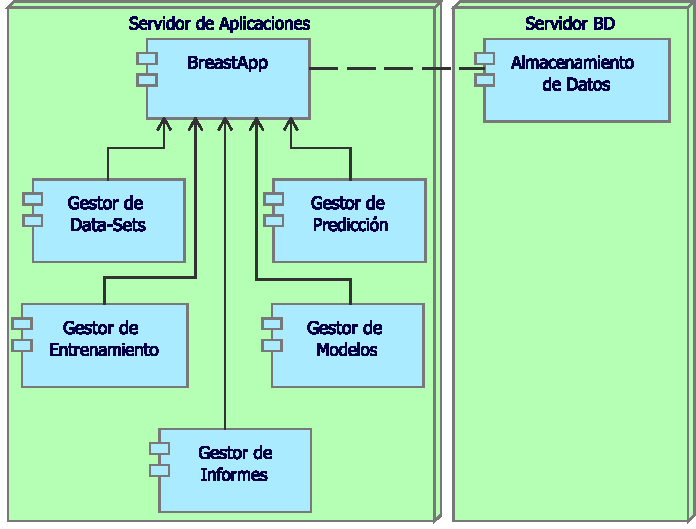
\includegraphics[width=1\linewidth]{ARQUITECTURA/imgs/CapaTecnologia/2_PvUsoInfraestructuraTec}
	\caption{Punto de Vista del Uso de la Infraestructura}
	\label{PvUsoInfraestructura}
\end{figure}


\begin{enumerate}[label=\textbf{\arabic*})]
\item  \textbf{Servidor de Aplicaciones:} En este servidor, interactúan diferentes componentes de la aplicación de BreastApp y se comunica con mas servidores a través de dichos componentes. Los componentes se describen a continuación:

\begin{itemize}
\item  \textbf{\textit{Gestor de Modelos:}} Este componente es usado por el componente principal de BreastApp.En este componente se maneja el proceso Crear modelos.
		
\item  \textbf{\textit{Gestor de Predicción:}}Este componente es usado por el componente principal de BreastApp.En este componente se maneja el proceso de diagnosticar el padecimiento de cáncer de mama.
			
\item  \textbf{\textit{Gestor de Data-Sets:}}Este componente es usado por el componente principal de BreastApp.En este componente se maneja el proceso de carga  y gestión de Data-Sets para ser almacenados en el sistema.
				
\item  \textbf{\textit{Gestor de Entrenamiento:}}Este componente es usado por el componente principal de BreastApp. En este componente se maneja el proceso de entrenamientos de los modelos de Machine Learning haciendo uso de los Data-Sets  que estén almacenados en el sistema.
					
\item  \textbf{\textit{Gestor de Informes:}}Este componente es usado por el componente principal BreastApp.En este componente se maneja el proceso de generar informes con detalles del diagnóstico.				
\end{itemize}

\item  \textbf{Servidor BD:}  Este sistema de software hace referencia a la persistencia de los datos de la aplicación BreastApp. Se realiza  automáticamente en el Back-End de la aplicación por medio del framework Django. Este servidor hace uso del componente que se describe a continuación:
\begin{itemize}
	\item  \textbf{\textit{Almacenamiento de Datos:}} Este componente hace referencia a la persistencia de la aplicación BrastApp. En este se desarrollan las funciones CRUD de la Capa de servicios REST implementada en el Back-End de la aplicación.
\end{itemize}

\end{enumerate}

%-------------Punto de Vista del Uso la Infraestructura----------%
\newpage
\section{Punto de Vista de Implementación y Organización}
El Punto de Vista de implementación y Organización describe como se despliegan una o más aplicaciones en la infraestructura. Este punto de vista comprende la asignación de aplicaciones y componentes lógicos a artefactos físicos \cite{BolanosCastro2019}.

En la Figura \ref{PvImpleOrg}, se plantea el Caso para el Punto de Vista de Implementación y Organización con cada uno de los elementos que interactúan entre sí. 

\begin{figure}[h!]
	\centering
	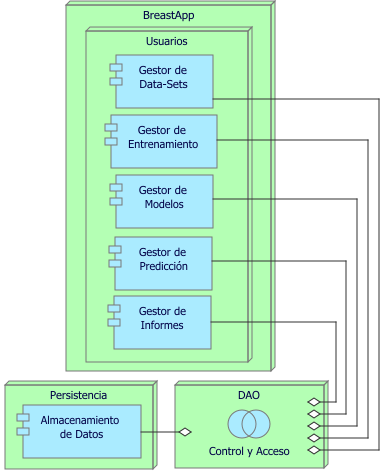
\includegraphics[width=0.65\linewidth]{ARQUITECTURA/imgs/CapaTecnologia/3_PvImplementacionOrganizacionTec}
	\caption{Punto de Vista de Implementación y Organización}
	\label{PvImpleOrg}
\end{figure}

\begin{enumerate}[label=\textbf{\arabic*})]
	
\item  \textbf{BreastApp:} Este sistema de Software representa a la aplicación en donde se desarrollan los componentes correspondientes para el diagnóstico de cáncer de mama. En este caso se tiene un nodo el cual interactúa con los componentes de este sistema.

\item  \textbf{Usuarios:} Este nodo contiene los componentes que tienen directa relación con los investigadores y unidades funcionales del Instituto de Cancerología y sus diferentes funciones. En este caso, se especifica un componente agregado a la colaboración de aplicación
\textit{Control} y \textit{Acceso}.

\begin{itemize}
\item  \textbf{\textit{Gestor de Modelos:}} En este componente se maneja el proceso de crear modelos de Machine Learning.
			
\item  \textbf{\textit{Gestor de Predicción:}} En este componente se maneja el proceso de diagnosticar el padecimiento de cáncer de mama.
				
\item  \textbf{\textit{Gestor de Data-Sets:}}En este componente se maneja el proceso de carga  y gestión de Data-Sets para ser almacenados en el sistema.
					
\item  \textbf{\textit{Gestor de Entrenamiento:}}En este componente se maneja el proceso de entrenamientos de los modelos de Machine Learning haciendo uso de los Data-Sets  que estén almacenados en el sistema.
						
\item  \textbf{\textit{Gestor de Informes:}}En este componente se maneja el proceso generar informes con detalles del diagnóstico.
\end{itemize}

\item  \textbf{Persistencia:} Este nodo hace referencia a la persistencia de la aplicación. Tiene el componente encargado de el almacenamiento y uso de información. Además, esta agregado a la colaboración de aplicación \textit{Control} y \textit{Acceso}.

\begin{itemize}
\item  \textbf{\textit{Almacenamiento de Datos:}} Este componente hace referencia a la persistencia de la aplicación BreastAPP. En este se desarrollan las funciones CRUD de la Capa de servicios REST implementada en el Back-End de la aplicación. 
\end{itemize} 

\item  \textbf{DAO:} Este sistema de software se refiere al componente que suministra la interfaz de comunicación entre la aplicación BreastApp y la base de datos. En este caso, se hace a través de una colaboración de aplicación, que se describe a continuación.

\begin{itemize}
	\item  \textbf{\textit{Control y Acceso:}} Esta colaboración trata del control de la información de las diferentes funciones de la aplicación BreastApp y su almacenamiento, y el acceso a dicha información. Tiene agregado los componentes de \textit{Gestor de Modelos},\textit{Gestor de Predicción}, \textit{Gestor de Data-Sets},\textit{Gestor de Entrenamiento}, \textit{Gestor de Informes} y \textit{Almacenamiento de Datos}.Esta colaboración es el puente para el CRUD de la Capa de servicios REST implementada en el Back-End de la aplicación BreastApp y el
	almacenamiento de los datos.
\end{itemize} 
\end{enumerate}
%-------------Punto de Vista de la Estructura de la Informacion----------%
\newpage
\section{Punto de Vista de Estructura de la Información}
El Punto de Vista de Estructura de la Información describe la estructura de la información usada en la empresa o en un proceso especifico de negocio o aplicación, en términos de tipos de datos o estructuras de clases \cite{BolanosCastro2019}.

En la Figura \ref{PvEstructuraInfo}, se plantea el Caso para el Punto de Vista de Estructura de la Información con cada uno de los elementos que interactúan entre sí. 

\begin{figure}[h!]
   \centering
   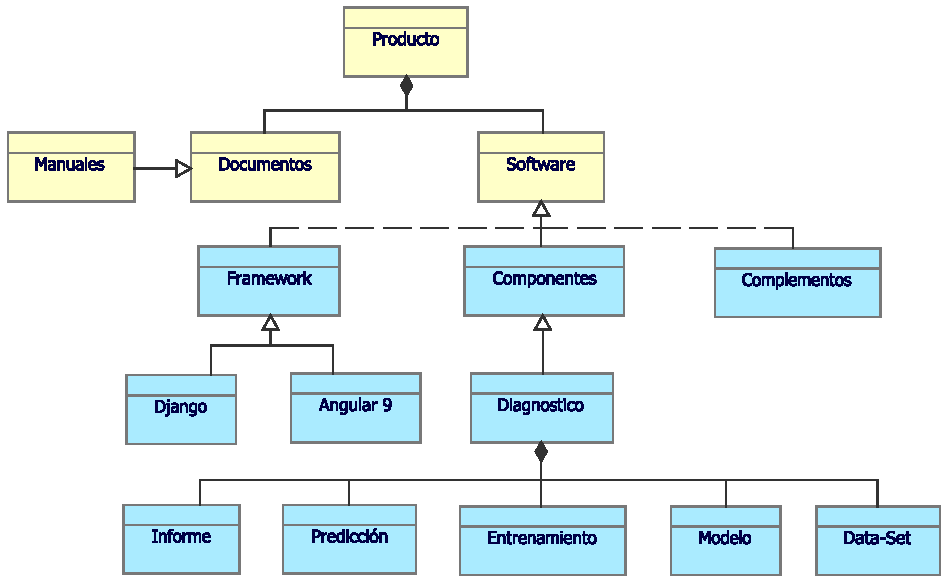
\includegraphics[width=1\linewidth]{ARQUITECTURA/imgs/CapaTecnologia/4_PvEstructuraInformacionTec}
	\caption{Punto de Vista de Estructura de Información}
	\label{PvEstructuraInfo}
\end{figure}

\begin{enumerate}[label=\textbf{\arabic*})]
	
\item  \textbf{Producto:} Este objeto de negocio se refiere al producto de software que se tiene en su totalidad. Este a su vez está compuesto por \textit{Documentos} y \textit{Software}.

\item  \textbf{Documentos:} Este objeto de negocio que hace referencia a toda la documentación correspondiente al producto como los \textit{Manuales}. Todo esto se va desarrollando gradualmente y se obtiene con el producto final.

\item  \textbf{Software:} Este objeto de negocio hace referencia a la implementación en software de la aplicación BreastApp. Este a su vez es realizado por diferentes objetos de negocio: \textit{Framework},\textit{Componentes} y \textit{Complementos}.

\item  \textbf{Framework:} En este objeto se desarrolla el software BreastApp. Esta conformado por el Framework \textit{Django} en el cual se realiza toda la lógica de la capa de servicios REST implementada en el Back-End y el Framework \textit{Angular 9} en el cual se pueden visualizar todas las funciones de la aplicación implementadas en el Front-End.

\item  \textbf{Componentes:} Este objeto contiene los diferentes componentes que interactúan en la aplicación BreastApp. Es una especialización del objeto \textit{Diagnostico} el cual es el resultado final de la aplicación y que se encuentra compuesto por los objetos \textit{Informe},\textit{Predicción},\textit{Entrenamiento},\textit{Modelo} y \textit{Data-Set}.

\item  \textbf{Complementos:} Este objeto que se refiere a los diferentes complementos utilizados en la aplicación BreastApp.En este caso se tienen complementos para la generación  de la persistencia de los datos, el diseño del Front y la publicación y consumo de la capa de servicios de la aplicación.
\end{enumerate}

%-------------Punto de Vista de Realización del Servicio----------%
\newpage
\section{Punto de Vista de Realización del Servicio}
El Punto de Vista de Realización de Servicio describe cómo uno o más servicios de negocio son realizados por un proceso fundamental o, algunas veces, por componentes de aplicación. Esto forma el puente entre productos  y las vistas de los procesos de negocio \cite{BolanosCastro2019}.

En la Figura \ref{PvRealizaServicio}, se plantea el Caso para el Punto de Vista de Realización del Servicio con cada uno de los elementos que interactúan entre sí. 

\begin{figure}[h!]
	\centering
	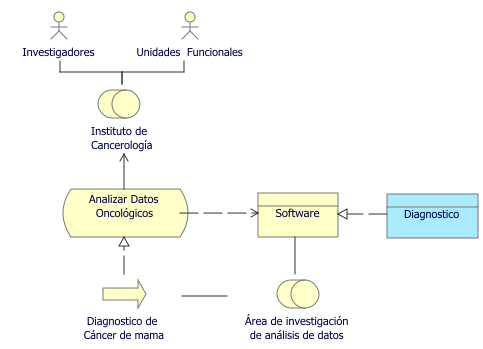
\includegraphics[width=1\linewidth]{ARQUITECTURA/imgs/CapaTecnologia/5_PvRealizacionServicioTec}
	\caption{Punto de Vista de Realización de Servicio}
	\label{PvRealizaServicio}
\end{figure}


\begin{enumerate}[label=\textbf{\arabic*})]
	
\item  \textbf{Analizar Datos Oncológicos:}  Este servicio realiza el análisis de los datos entregados por  los investigadores de la Subdirección de Investigaciones, otras Subdirecciones y demás unidades funcionales del Instituto de Cancerología para generar diagnósticos oncológicos. Es realizado por el proceso de \textit{Diagnostico de Cáncer de mama} y usado por el \textit{Instituto de Cancerología}.

\item  \textbf{Diagnostico de Cáncer de mama:}  Este proceso cumple el objetivo dar soporte a los investigadores de la Subdirección de Investigaciones, otras Subdirecciones y demás unidades funcionales del Instituto de Cancerología con respecto al análisis de datos oncológicos. Tiene asignado el rol \textit{Área de investigación de análisis de datos}.

\item  \textbf{Área de investigación de análisis de datos:}  Corresponde al área de investigación la cual da soporte a los investigadores de la Subdirección de Investigaciones, otras Subdirecciones y demás unidades funcionales del Instituto de Cancerología por medio reportes generados con base a los datos solicitados.Esta asignado al proceso \textit{Diagnostico de Cáncer de mama}.

\item  \textbf{Instituto de Cancerología :} Este rol de aplicación corresponde a los diferentes usuarios del Instituto de Cancerología. Tienes asociado el actor \textit{Investigadores} y el actor \textit{Unidades funcionales }. Estos roles se describen a continuación: 
\begin{itemize}
	\item  \textbf{\textit{Investigadores :}}  Este rol está conformado por todos los grupos de investigación en cáncer del país registrados ante Colciencias y adicionalmente, con representantes de diferentes tipos de usuarios del conocimiento generado por la investigación como son las sociedades médicas, los prestadores de servicios oncológicos, los aseguradores, las autoridades sanitarias y los pacientes entre otros. 
	
	\item  \textbf{\textit{Unidades Funcionales :}}  Este rol está conformado por las unidades clínicas ubicadas al interior del Instituto de Cancerología cuya función es evaluar la situación de salud del paciente con diagnóstico presuntivo de cáncer. 
\end{itemize}

\item  \textbf{Software:} Este objeto de negocio hace referencia a la implementación en software de la aplicación BreastApp. Es realizado por el objeto \textit{Diagnostico}.
\end{enumerate}

%-------------Punto de Vista de Capas----------------------------------%
\newpage
\section{Punto de Vista de Capas}
El Punto de Vista de capas describe varias los aspectos de una arquitectura empresarial en un diagrama como resultado del uso de la relación de agrupación para  una partición natural de todo el conjunto de objetos y relaciones que pertenecen a el modelo \cite{BolanosCastro2019}.

En la Figura \ref{PvCapas}, se plantea el Caso para el Punto de Vista de Capas con cada uno de los elementos que interactúan entre sí. 

\begin{figure}[h!]
	\centering
	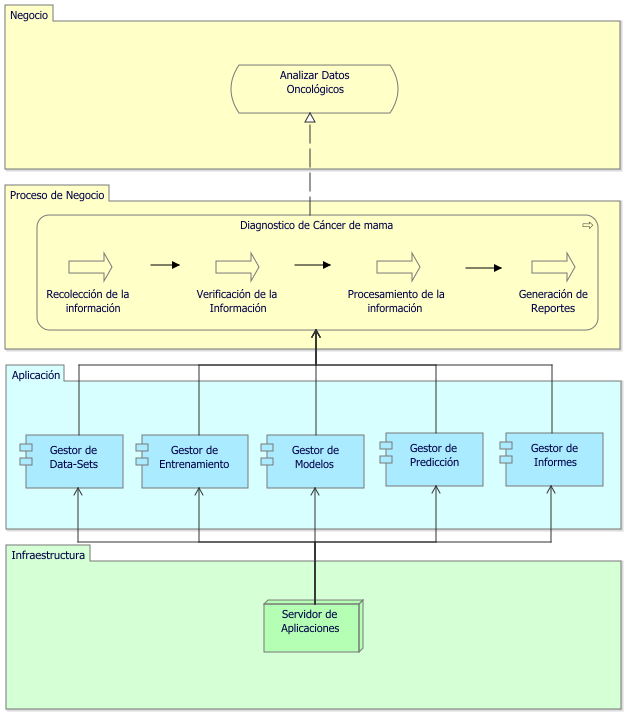
\includegraphics[width=0.8\linewidth]{ARQUITECTURA/imgs/CapaTecnologia/6_PvCapasTec}
	\caption{Punto de Vista de Capas}
	\label{PvCapas}
\end{figure}

\begin{enumerate}[label=\textbf{\arabic*})]
	
\item  \textbf{Negocio:} Esta capa expone un servicio importante el cual fue planteado con anterioridad en la Capa de Negocio. Estos  servicio es realizado por un proceso especifico, expuesto en la siguiente capa del modelo de Proceso de Negocio. La descripción de los servicios
	se expone a continuación:
	\begin{itemize}
		\item  \textbf{\textit{Analizar Datos Oncológicos:}} Este servicio realiza el análisis de los datos entregados por  los investigadores de la Subdirección de Investigaciones, otras Subdirecciones y demás unidades funcionales del Instituto de Cancerología para generar diagnósticos oncológicos.Es realizado por el proceso de \textit{Diagnostico de Cáncer de mama}.
	\end{itemize}

\item  \textbf{Proceso de Negocio:} Esta capa, expone los procesos encargados de realizar los servicios expuestos en el entorno. Son usados por distintos componentes planteados en la capa de Aplicación. La descripción de los procesos se expone a continuación.
	
	\begin{itemize}
	\item  \textbf{Diagnostico de Cáncer de mama:}  Este proceso cumple el objetivo dar soporte a los investigadores de la Subdirección de Investigaciones, otras Subdirecciones y demás unidades funcionales del Instituto de Cancerología con respecto al análisis de datos oncológicos. Esta compuesto de los siguientes procesos de negocio secuenciales: \textit{Recolección de información},\textit{Verificación de la información},\textit{Procesamiento de la información} y \textit{Generación  de Reportes}.
	\end{itemize}


\item  \textbf{Aplicación:} Esta capa, plantea los diferentes componentes que usan los procesos de negocio expuestos en la capa de Aplicación. A su vez, son usados en la capa siguiente, a través de un nodo. Esta capa esta conformada de por los siguientes componentes:

\begin{itemize}
	\item  \textbf{\textit{Gestor de Modelos:}} En este componente se maneja el proceso de crear modelos de Machine Learning.
	
	\item  \textbf{\textit{Gestor de Predicción:}} En este componente se maneja el proceso de diagnosticar el padecimiento de cáncer de mama.
	
	\item  \textbf{\textit{Gestor de Data-Sets:}} En este componente se maneja el proceso de carga  y gestión de Data-Sets para ser almacenados en el sistema.
	
	\item  \textbf{\textit{Gestor de Entrenamiento:}} En este componente se maneja el proceso de entrenamientos de los modelos de Machine Learning haciendo uso de los Data-Sets  que estén almacenados en el sistema.
	
	\item  \textbf{\textit{Gestor de Informes:}} En este componente se maneja el proceso generar informes con detalles del diagnóstico.
\end{itemize}

\item  \textbf{Infraestructura:} En esta Capa, se plantea el nodo Servidor de Aplicaciones, que usa los diferentes componentes planteados en la Capa de Aplicación. El nodo, se describe a continuación:

\begin{itemize}
\item  \textbf{Servidor de Aplicaciones:} Hace referencia a el nodo que se conecta directamente a la red para exponer la disponibilidad de la aplicación. Es el nodo general donde interactúan tanto componentes, como sistemas de software y demás elementos necesarios para la aplicación. Los componentes usados de la capa de aplicación por este nodo son: \textit{Gestor de Modelos},\textit{Gestor de Predicción}, \textit{Gestor de Data-Sets},\textit{Gestor de Entrenamiento} y \textit{Gestor de Informes}.
\end{itemize}
	
\end{enumerate}

	\chapter{Capa de Migración e Implementación}
\section{Introducción}
Esta capa describe la implementación de modelos y características de migración para   ejecutar un cambio en la arquitectura del negocio. Cada uno de los puntos de vista que contiene esta capa presenta una perspectiva  para modelar la gestión del cambio de arquitectura, modelar la transición de una arquitectura existente a una arquitectura de destino y definir las relaciones entre los programas y proyectos y las partes de la arquitectura que implementan \cite{ArchiMate3.0.1}. 

Esta capa da conocer el contexto sobre el cual se busca modelar el cambio estructural de la arquitectura empresarial. Para una adecuada apropiación de la conceptualización de esta capa, se implementa el uso de tres diferentes puntos de vista (proyecto,migración y migración e implementación). En esta capa se retoman algunos de los conceptos utilizados en la capa de negocio como por ejemplo el concepto de objeto de negocio representado en esta capa como un Paquete de Trabajo
(Work Package) y el concepto de representación el cual tiene como
equivalente un Liberable (Derivable)\cite{BolanosCastro2019}.


A continuación se presentan cada uno de los puntos de vista de la capa de Implementación a partir del soporte realizado por el Área de Investigación de Análisis de datos a los investigadores de la Subdirección de Investigaciones, otras Subdirecciones y demás unidades funcionales del Instituto de Cancerología.

%-------------Punto de Vista de Proyecto----------%
\newpage
\section{Punto de Vista de Proyecto}
El punto de vista de proyecto se utiliza principalmente para modelar la gestión del cambio de la arquitectura permitiendo al diseñador o analista plasmar mediante un diagrama el proceso de interacción de los diferentes elementos\cite{BolanosCastro2019}. 

En la Figura \ref{PvProyecto} se plantea el Caso para el Punto de Vista de Proyecto con cada uno de los elementos que interactúan entre sí. 

\begin{figure}[h!]
	\centering
	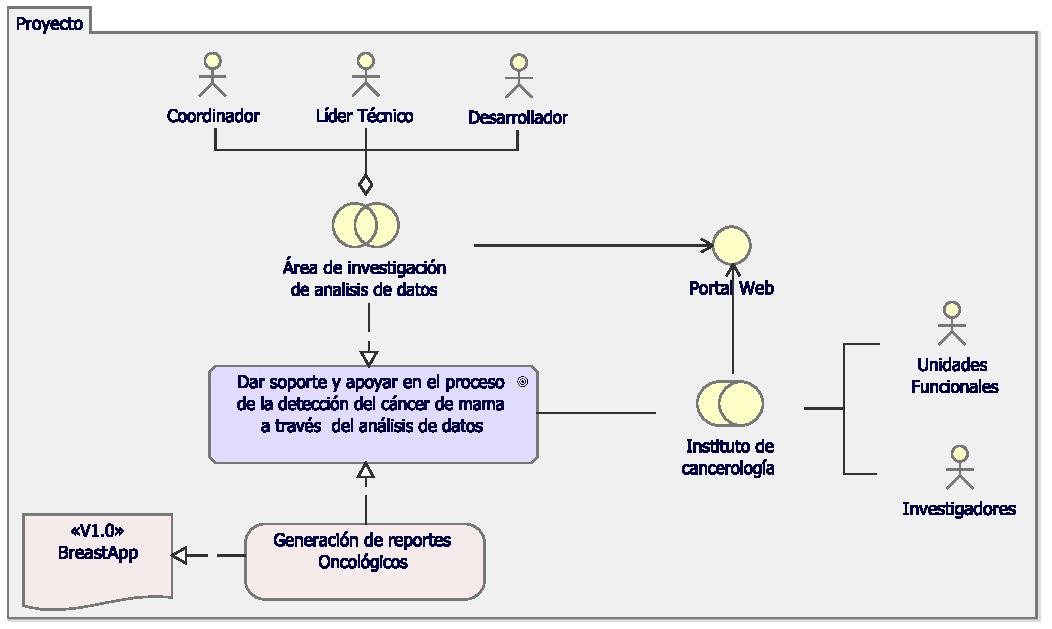
\includegraphics[width=1\linewidth]{ARQUITECTURA/imgs/CapaImplementacion/1_PvProyecto}
	\caption{Punto de Vista de Proyecto}
	\label{PvProyecto}
\end{figure}

\begin{enumerate}[label=\textbf{\arabic*})]

\item  \textbf{\textbf{Instituto  de Cancerología}:} Este elemento hace referencia a el rol de la organización el cual cuenta con siete grupos de investigación que desarrollan diversas actividades según su campo de acción: investigación clínica, investigación epidemológica, biología del cáncer e investigación en el área de la salud pública.A este rol están asociados el actor \textit{Investigador } y el actor \textit{Unidades funcionales }. Estos roles se describen a continuación: 
\newpage
\begin{itemize}
	\item  \textbf{\textit{Investigadores :}}  Este rol está conformado por todos los grupos de investigación en cáncer del país registrados ante Colciencias y adicionalmente, con representantes de diferentes tipos de usuarios del conocimiento generado por la investigación como son las sociedades médicas, los prestadores de servicios oncológicos, los aseguradores, las autoridades sanitarias y los pacientes entre otros. 
	
	\item  \textbf{\textit{Unidades Funcionales :}}  Este rol está conformado por las unidades clínicas ubicadas al interior del Instituto  de Cancerología cuya función es evaluar la situación de salud del paciente con diagnóstico presuntivo de cáncer. 
\end{itemize}

\item \textbf{Área de Investigación de análisis de datos:} Corresponde a una de las dependencias del área de investigación la cual  tiene por objetivo dar soporte a los investigadores de la Subdirección de Investigaciones, otras Subdirecciones y demás unidades funcionales del Instituto  de Cancerología, haciendo uso de métodos computacionales para el manejo y análisis de datos Oncológicos. Este actor tiene \textit{agregado} tres actores los cuales se muestran a continuación:

\begin{itemize}
\item  \textbf{\textit{Coordinador:}}
Es la persona encargada de regular, gestionar, dirigir y supervisar el Área de Investigación de análisis de datos de Oncología para que el soporte realizado a los investigadores de la Subdirección de Investigaciones, otras Subdirecciones y demás unidades funcionales se realice correctamente.
		
\item  \textbf{\textit{Líder Técnico:}}
Es la persona con conocimiento técnico avanzado en los temas de análisis de datos de Oncología y es el  responsable de asignar y definir las  tareas y el tiempo necesario en el desarrollo e implementación de los recursos  según las necesidades presentadas por los investigadores y las unidades funcionales del Instituto  de Cancerología.

\item  \textbf{\textit{Desarrollador:}}
Es la persona encargada de cumplir con las implementaciones presentadas en el ámbito de análisis de datos de Oncología y que da  solución a cada uno de los requerimientos y necesidades presentadas por los  investigadores y las unidades funcionales del Instituto  de Cancerología.
\end{itemize}

\item  \textbf{Portal Web :} Es el medio de comunicación entre el Área de Investigación de análisis de datos  y los investigadores de la Subdirección de Investigaciones, otras Subdirecciones y demás unidades funcionales del Instituto  de Cancerología. Esta interfaz tiene una asociación con el rol del  \textit{Área de Investigación de análisis de datos}  y es usada por el rol \textit{Instituto  de Cancerología}.


\item  \textbf{Dar soporte y apoyar en el proceso de la detección del cáncer de mama a través del análisis de datos:} Este objetivo organizacional hace referencia a el servicio de generar diagnósticos relacionados con el cáncer de mama  solicitados por los diferentes funcionarios del Instituto de Cancerología.

\item  \textbf{Generación de reportes oncológicos:} Es el paquete de trabajo principal del instituto de Cancerología basado en la estrategia planteada y los recursos disponibles identificados. La meta es construir una  aplicación web que genere  informes tipo reporte con base a los resultados arrojados por  diferentes modelos de Machine Learning, en donde se de un resultado definitivo acerca del  padecimiento de Cáncer de mama.Este diagnostico se realiza con el propósito de dar soporte a los investigadores de la Subdirección de Investigaciones, otras Subdirecciones y demás unidades funcionales del Instituto  de Cancerología.

\item  \textbf{BreastApp:} Representa el liberable, consecuencia del paquete de
trabajo definido anteriormente. Este producto corresponde a la generación de reportes diagnósticos según el análisis de datos oncológicos elaborados por los investigadores de la Subdirección de Investigaciones, otras Subdirecciones y demás unidades funcionales del Instituto  de Cancerología.Es el resultado obtenido que cumple con los objetivos planteados y satisface las necesidades de la organización.
\end{enumerate}

%-------------Punto de Vista de Migracion----------%
\newpage
\section{Punto de Vista de Migración}
El Punto de Vista de Migración implica modelos y conceptos que pueden usarse para especificar la transición de una arquitectura existente a una arquitectura deseada.\cite{BolanosCastro2019}. 

En la Figura \ref{PvMigracion} se plantea el Caso para el Punto de Vista de Migración con cada uno de los elementos que interactúan entre sí. 

\begin{figure}[h!]
	\centering
	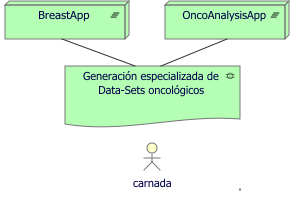
\includegraphics[width=0.75\linewidth]{ARQUITECTURA/imgs/CapaImplementacion/2_PvMigracion}
	\caption{Punto de Vista de Migración}
	\label{PvMigracion}
\end{figure}

\begin{enumerate}[label=\textbf{\arabic*})]
	
\item  \textbf{BreastApp:} Es la Meseta inicial que  corresponde  a una aplicación web la cual genera reportes diagnósticos según el análisis de datos relacionados con el Cáncer de mama elaborados para brindar soporte a los investigadores de la Subdirección de Investigaciones, otras Subdirecciones y demás unidades funcionales del Instituto  de Cancerología.

\item  \textbf{Generación especializada de  Data-Sets oncológicos:} Hace referencia a la brecha que debe resolverse para poder generar la Meseta futura \textit{OncoAnalysisApp}.Esta brecha esta relacionada con la generación dinámica de Data-Sets para cualquier tipo de cáncer.

\item  \textbf{OncoAnalysisApp:} Es la Meseta final de la aplicación. Representa un producto a futuro con nuevas implementaciones y funcionalidades adicionales. En este caso se pretende generar diagnósticos para cualquier tipo de cáncer para brindar un soporte mas amplio a los investigadores de la Subdirección de Investigaciones, otras Subdirecciones y demás unidades funcionales del Instituto  de Cancerología

\end{enumerate}

%-------------Punto de Vista de Migracion----------%
\newpage
\section{Punto de Vista de Migración e implementación}
El Punto de Vista de Migración e Implementación se utiliza para relacionar programas y proyectos con las partes de la arquitectura que implementan\cite{BolanosCastro2019}. 

En la Figura \ref{PvMigraImple} se plantea el Caso para el Punto de Vista de Migración con cada uno de los elementos que interactúan entre sí. 

\begin{figure}[h!]
	\centering
	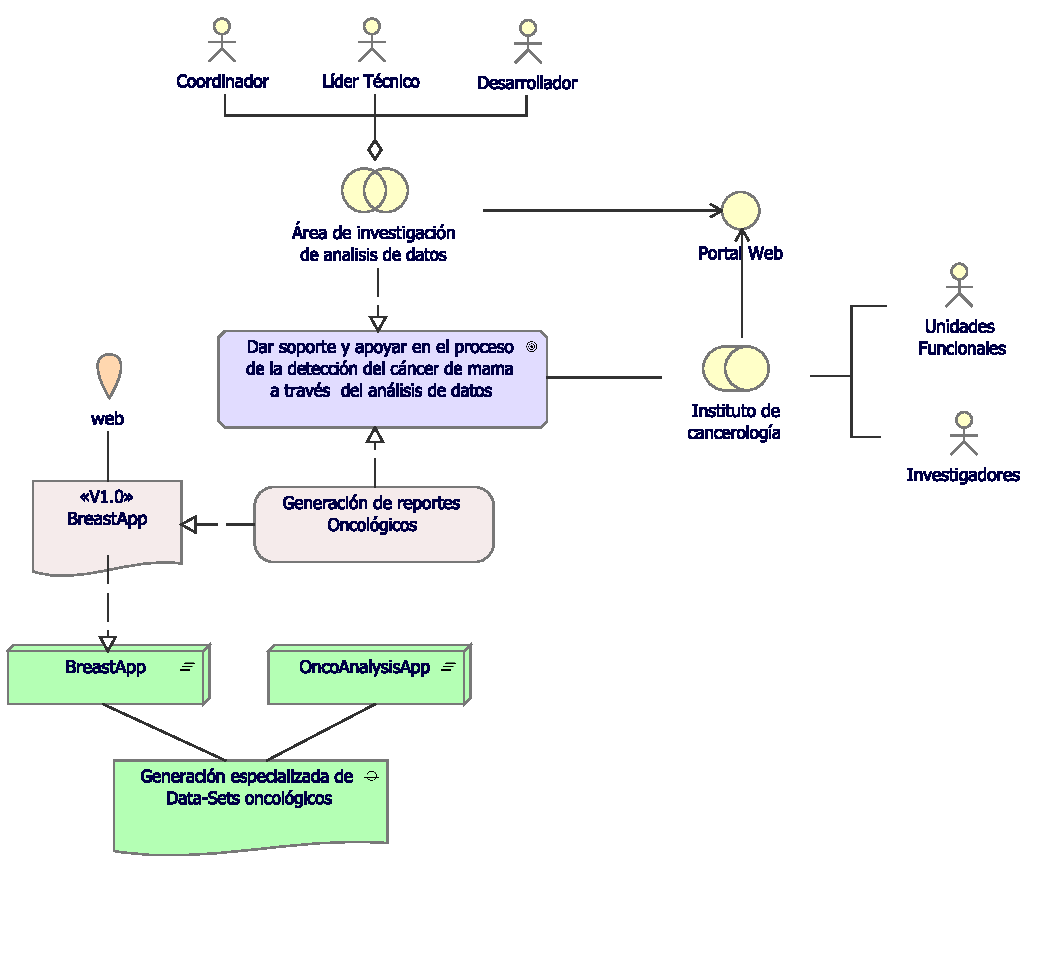
\includegraphics[width=0.92\linewidth]{ARQUITECTURA/imgs/CapaImplementacion/3_PvMigracionImplementacion}
	\caption{Punto de Vista de Migración e Implementación}
	\label{PvMigraImple}
\end{figure}

\begin{enumerate}[label=\textbf{\arabic*})]
	
	\item  \textbf{\textbf{Instituto  de Cancerología}:} Este elemento hace referencia a el rol de la organización el cual cuenta con siete grupos de investigación que desarrollan diversas actividades según su campo de acción: investigación clínica, investigación epidemológica, biología del cáncer e investigación en el área de la salud pública.A este rol están asociados el actor \textit{Investigador } y el actor \textit{Unidades funcionales }. Estos roles se describen a continuación: 
	\begin{itemize}
		\item  \textbf{\textit{Investigadores :}}  Este rol está conformado por todos los grupos de investigación en cáncer del país registrados ante Colciencias y adicionalmente, con representantes de diferentes tipos de usuarios del conocimiento generado por la investigación como son las sociedades médicas, los prestadores de servicios oncológicos, los aseguradores, las autoridades sanitarias y los pacientes entre otros. 
		
		\item  \textbf{\textit{Unidades Funcionales :}}  Este rol está conformado por las unidades clínicas ubicadas al interior del Instituto  de Cancerología cuya función es evaluar la situación de salud del paciente con diagnóstico presuntivo de cáncer. 
	\end{itemize}
	
	\item \textbf{Área de Investigación de análisis de datos:} Corresponde a una de las dependencias del área de investigación la cual  tiene por objetivo dar soporte a los investigadores de la Subdirección de Investigaciones, otras Subdirecciones y demás unidades funcionales del Instituto  de Cancerología, haciendo uso de métodos computacionales para el manejo y análisis de datos Oncológicos. Este actor tiene \textit{agregado} tres actores los cuales se muestran a continuación:
	
	\begin{itemize}
		\item  \textbf{\textit{Coordinador:}}
		Es la persona encargada de regular, gestionar, dirigir y supervisar el Área de Investigación de análisis de datos de Oncología para que el soporte realizado a los investigadores de la Subdirección de Investigaciones, otras Subdirecciones y demás unidades funcionales se realice correctamente.
		
		\item  \textbf{\textit{Líder Técnico:}}
		Es la persona con conocimiento técnico avanzado en los temas de análisis de datos de Oncología y es el  responsable de asignar y definir las  tareas y el tiempo necesario en el desarrollo e implementación de los recursos  según las necesidades presentadas por los investigadores y las unidades funcionales del Instituto  de Cancerología.
		
		\item  \textbf{\textit{Desarrollador:}}
		Es la persona encargada de cumplir con las implementaciones presentadas en el ámbito de análisis de datos de Oncología y que da  solución a cada uno de los requerimientos y necesidades presentadas por los  investigadores y las unidades funcionales del Instituto  de Cancerología.
	\end{itemize}
	
	\item  \textbf{Portal Web :} Es el medio de comunicación entre el Área de Investigación de análisis de datos  y los investigadores de la Subdirección de Investigaciones, otras Subdirecciones y demás unidades funcionales del Instituto  de Cancerología. Esta interfaz tiene una asociación con el rol del  \textit{Área de Investigación de análisis de datos}  y es usada por el rol \textit{Instituto  de Cancerología}.
	
	
	\item  \textbf{Dar soporte y apoyar en el proceso de la detección del cáncer de mama a través del análisis de datos:} Este objetivo organizacional hace referencia a el servicio de generar diagnósticos relacionados con el cáncer de mama  solicitados por los diferentes funcionarios del Instituto de Cancerología.
	
	\item  \textbf{Generación de reportes oncológicos:} Es el paquete de trabajo principal del instituto de Cancerología basado en la estrategia planteada y los recursos disponibles identificados. La meta es construir una  aplicación web que genere  informes tipo reporte con base a los resultados arrojados por  diferentes modelos de Machine Learning, en donde se de un resultado definitivo acerca del  padecimiento de Cáncer de mama.Este diagnostico se realiza con el propósito de dar soporte a los investigadores de la Subdirección de Investigaciones, otras Subdirecciones y demás unidades funcionales del Instituto  de Cancerología.
	
	\item  \textbf{BreastApp:} Representa el liberable, consecuencia del paquete de trabajo definido anteriormente. Este producto corresponde a la generación de reportes diagnósticos según el análisis de datos oncológicos elaborados por los investigadores de la Subdirección de Investigaciones, otras Subdirecciones y demás unidades funcionales del Instituto  de Cancerología.Es el resultado obtenido que cumple con los objetivos planteados y satisface las necesidades de la organización. Realiza a la Meseta inicial \textit{BreastApp}
	
	\item  \textbf{Generación especializada de  Data-Sets oncológicos:} Hace referencia a la brecha que debe resolverse para poder generar la Meseta futura \textit{OncoAnalysisApp}.Esta brecha esta relacionada con la generación dinámica de Data-Sets para cualquier tipo de cáncer.
	
	\item  \textbf{OncoAnalysisApp:} Es la Meseta final de la aplicación. Representa un producto a futuro con nuevas implementaciones y funcionalidades adicionales. En este caso se pretende generar diagnósticos para cualquier tipo de cáncer para brindar un soporte mas amplio a los investigadores de la Subdirección de Investigaciones, otras Subdirecciones y demás unidades funcionales del Instituto  de Cancerología
	
	\item  \textbf{Web:} Hace referencia a la ubicación en donde los investigadores de la Subdirección de Investigaciones, otras Subdirecciones y demás unidades funcionales del Instituto de Cancerología pueden acceder a la aplicación \textit{BreastApp}.
\end{enumerate}




	\part{ANÁLISIS Y RESULTADOS}
	\chapter{Análisis}
	\chapter{Resultados}

	%--------------------[III] REFLEXIONES------------------------------
	%\part{REFLEXIONES}
	%\include{REFLEXIONES/resultados}
	
	%--------------------[IV]BIBLIOGRAFIA-------------------------------
	\bibliographystyle{unsrt}
	\bibliography{REFERENCIAS/articulos}
	%\include{PROYECTO/Desarrollo}
	
	
\end{document}